\documentclass[a4paper,12pt, english,twoside]{book}% norsk istedefor english
%\usepackage{ucs}
\usepackage[utf8]{inputenc}%utf8x
\usepackage{fontenc}%[T1]
\usepackage{babel,graphicx,subfigure,epsfig}%,uioforside},babel hvis norsk
\usepackage{amssymb,psfrag,amsmath,wick}
\usepackage{wrapfig,algorithm,algorithmic}
\usepackage{verbatim}
%\usepackage{a4wide}
\usepackage{bezier}
\usepackage{color}  
\usepackage[pdftex,colorlinks=true,bookmarks=true,linkcolor=blue]{hyperref}

\newcommand{\be}{ \begin{equation}}
\newcommand{\ee}{ \end{equation}}
\newcommand{\mc}{ \mathcal }
\newcommand{\bra}[1]{\langle #1|}
\newcommand{\ket}[1]{|#1\rangle}
\newcommand{\braket}[2]{\langle #1|#2\rangle}
\newcommand{\beq}{\begin{equation*}}
\newcommand{\eeq}{\end{equation*}}
\newcommand{\ds}{\displaystyle{\not}}
\newcommand{\bsp}{\begin{split}}
\newcommand{\eesp}{\end{split}}
\newcommand{\matr}[1]{{\bf \cal{#1}}}
\newcommand{\OP}[1]{{\bf\widehat{#1}}}
\newcommand{\sd}{$}

%\title{AB INITIO STUDIES OF INFINITE MATTER}
%\author{Johannes Rekkedal}
%\date{}


 \renewcommand{\rmdefault}{ptm} % Times
 \newcommand{\clearemptydoublepage}{\newpage{\pagestyle{empty}\cleardoublepage}}
 \newcommand{\mymarkright}[1]{\markright{\thesection\ -- #1}}
 \newcommand{\mymarkboth}[2]{\markboth{#1}{#2}}
 %
 % redefine page style
 %
 \usepackage{fancyhdr}
 % choose pagestyle fancy and define it
 \pagestyle{fancy}
 \fancyhead{} %clear everything
 \fancyfoot{} %clear everything
 \addtolength{\headheight}{1.5pt}
 \addtolength{\headwidth}{2.5\marginparsep}
 \renewcommand{\chaptermark}[1]{\mymarkboth{#1}{}}
 \renewcommand{\sectionmark}[1]{\mymarkright{#1}}
 \fancyfoot[EL,OR]{\bfseries\itshape\thepage}
 \fancyhead[EL]{\nouppercase{\bfseries\itshape\leftmark}}
 \fancyhead[OR]{\nouppercase{\bfseries\itshape\rightmark}}
 \renewcommand{\headrulewidth}{1pt}
 % redefine plain page style. used on first pages of chapters et.c.
 \fancypagestyle{plain}{\fancyhf{}\fancyfoot[EL,OR]{\bfseries\itshape\thepage}%
 \renewcommand{\headrulewidth}{0pt}
 }
 %
 % redefine bullet. looks better with an ndash.
 %
 \renewcommand{\labelitemi}{\bfseries--}
 %
 % define styles for section and subsection headings
 %
 %\font\tenhv  = phvb at 12pt
 %\newcommand{\hvfont}{\fontfamily{phv}\selectfont}
 %\newcommand{\hvfont}{\fontfamily{phv}\fontseries{bc}\selectfont}
 \newcommand{\secstyle}{\normalfont\itshape\bfseries\large}
 %\newcommand{\secstyle}{\hvfont\itshape\large}
 \newcommand{\subsecstyle}{\normalfont\itshape\large}
 \newcommand{\paragraphstyle}{\normalfont\itshape}
 %
 % redefine look of sections, subsections and paragraphs.
 %

\makeatletter
 \renewcommand{\section}{%
 \@startsection
   {section}%   the name
   {1}%         the level
   {0pt} %{-\Myindent}%       the indent
   {-2\baselineskip}%   beforeskip
   {\baselineskip}%    afterskip
   {\secstyle}}%   style
 \renewcommand{\subsection}{%
 \@startsection
   {subsection}%   the name
   {2}%         the level
   {0pt}%{-\Myindent}%       the indent
   {-\baselineskip}%   beforeskip
   {0.5\baselineskip}%    afterskip
   {\subsecstyle}}%   style
 \renewcommand{\paragraph}{%
 \@startsection
   {paragraph}%   the name
   {4}%         the level
   {0pt}%{-\Myindent}%       the indent
   {-\baselineskip}%   beforeskip
   {-1em}%    afterskip
   {\paragraphstyle}}%   style
 \makeatother
 %%
 %% modify margins...
 %%
 \addtolength{\oddsidemargin}{-0.5cm}
 \addtolength{\evensidemargin}{-1.0cm}
 \addtolength{\textwidth}{0.5cm}


\begin{document}
%\maketitle
\begin{titlepage}
\begin{center}
{\huge \bf Studies of quantum dots}\\
\ \\
{\Large \bf Ab initio coupled-cluster analysis using OpenCL and GPU programming}\\ 
\ \\ 
{\Large by}\\
\ \\
{\Large \bf Christoffer Hirth}\\
\ \\
\ \\
\ \\
{\large \bf THESIS}\\
{\large for the degree of}\\
{\large \bf MASTER OF SCIENCE}\\
\ \\
(Master in Computational Physics)\\
\ \\
\ \\
\begin{figure}[h!]
\begin{center}

\includegraphics[width=0.3\textwidth]{uiologo.eps}
\end{center}
\end{figure}
\ \\
\Large{\rm Faculty of Mathematics and Natural Sciences}\\
{\rm Department of Physics}\\
{\rm University of Oslo}\\
\ \\
\ \\
{\rm June 2012}
\end{center}
\end{titlepage}

\clearemptydoublepage
%\fysikkforside{}
%\uioforside[inst = Department of Physics]
% maa kompilere med latex istedefor pdflatex for at uioforside 
%skal virke
%\pagenumbering{roman}
\include{acknowledgement}
\clearemptydoublepage
\chapter*{Notation}

\section*{Units}
We will in all chapters except the second, regarding quantum mechanics, work with units, where
\beq
\hbar=c=1
\eeq
In this system,
\begin{align}
		&\mbox{[length]}=\mbox{[time]}=\mbox{[energy]}^{-1}=\mbox{[mass]}^{-1}.\notag
\end{align}
The mass $m$ of a particle is therefore equal to its rest energy ($mc^2$).

\section*{Vectors}
Vectors are boldfaced, $\bold v$ is an ordinary vector in three dimensions. Four vectors are denoted by a Greek letter, $A^\mu$, where $\mu=(0,1,2,3)$
\beq
A^\mu=\left(A^0,\bold A\right)~\mbox{and}~ A_\mu=(-A^0,\bold A)
\eeq


\section*{Summation convention}
We use Einstein summation conventions, where equal upper and lower indices are summed over, Greek letters are summed from zero to three,
\beq
A^\mu B_\mu=\sum_{\mu=0}^3A^\mu B_\mu.
\eeq

\section*{Spin and isospin}
The Pauli spin matrices $\mathbf\sigma$ are defined as
\beq
\sigma^i=\begin{pmatrix} 0 & 1\\1 & 0\end{pmatrix},~
		\sigma^j=\begin{pmatrix} 0 & -i\\i & 0\end{pmatrix}~\mbox{and}~
				\sigma^k=\begin{pmatrix} 1&0\\0&-1\end{pmatrix}.		
\eeq
The isospin matrices $\mathbf\tau$ are defined as 
\beq
\tau^i=\begin{pmatrix} 0 & 1\\1 & 0\end{pmatrix},~
		\tau^j=\begin{pmatrix} 0 & -i\\i & 0\end{pmatrix}~\mbox{and}~
				\tau^k=\begin{pmatrix} 1&0\\0&-1\end{pmatrix}.		
\eeq
\section*{Commutators}
A commutator between two operators $A$ and $B$  is defined as
\beq
[A,B]=AB-BA.
\eeq
The anticommutator is defined as
\beq
\{A,B\}=AB+BA.
\eeq

\clearemptydoublepage
\tableofcontents
\clearemptydoublepage
%\listoffigures
%\listoftables


%\pagenumbering{arabic}
\chapter{Introduction}
\label{introduction}

\section{Historical Background}

About 2400 years ago, the Greek philosopher Anaxagoras invented the
idea that matter could be devided into infinitly small parts;
\emph{spermata}. 
This concept was expanded a few years later by
Democritus, who believed matter was composed of tiny particles of
finite size or mass. He called the invisible particles of matter
\emph{atoms}; which in greek means 'undevidable'. 
No experimental techniques needed to test the atomic
hypotheses existed at the time, and there was no advance in the
understanding of atoms for more than 2000 years! 

\subsection*{Discovery of the Atom}

In 1807, John Dalton postulated that atoms of each element had a
unique mass. Dalton's atomic theory contained a simple prediction for
the case where two elements combine to form two different compounds;
\emph{The Law of Multiple Proportions}. (For example, 16 g of oxygen, O,
combines with 12 g of carbon, C, to form carbonmonoxide, CO, and
32 g of O combines with 12 g of C to form carbondioxide, CO$_2$).
%
\newline
%
A great leap in the understanding of the structure of matter was made
in 1811 by Amedeo Avogadro. Avogadro correctly hypothesized that the
particles of a gas were small compared to the distance between the
particles. He determined that these particles were often made up of
more than one atom; \emph{molecules}. This important result is the
basis for the \emph{Ideal Gas Law}, and the discovery provided a
systematic method for measurement of the atomic mass numbers.

\subsection*{The Periodic Table}

In 1869, Dmitri Mendeleev made the first classification of the
elements. The elements were ordered with increasing atomic mass
number, and placed in several columns according to their chemical
properties. Mendeleev discovered some gaps, that made him to correctly
predict the existance of undiscovered elements!

\subsection*{Discovery of the Electron}

A type of radiation, called \emph{cathode rays}, was observed to be
emitted from metallic surfaces when voltage was applied. At the end of
the 19$^{th}$ century there was much speculation about the fundamental
properties of the cathode rays. One school of thought held the belief
that cathode rays were particles, while the other school believed it
was a wave-phenomenon. In 1897, Joseph John Thomson preformed a
definitive set of experiments that proved that cathode rays had
a particle behavior. Thomson developed the necessary technique to
observe the deflection of chatode rays in an electric field. This led
to the interpretation of chatode rays as charged particles;
\emph{electrons}.

\subsection*{Measurement of the Electric Charge}

In 1909, Robert Millikan made the first accurate measurement of the
electron charge. \emph{The Millikan Oil-Droplet Experiment} was
performed by spraying tiny droplets of oil between two conducting
plates. By switching the electric field between the two plates on and
off, Millikan was able to accuratly estimate the electron charge. The
result of numerous measurements by Millikan, was that the charge was
allways an integer multiple of $1.6 \cdot 10^{-19}C$.
Figure \ref{oil_droplet} illustrates the forces acting on the
oil-droplet.

\begin{figure}[hbtp]
\begin{center}
  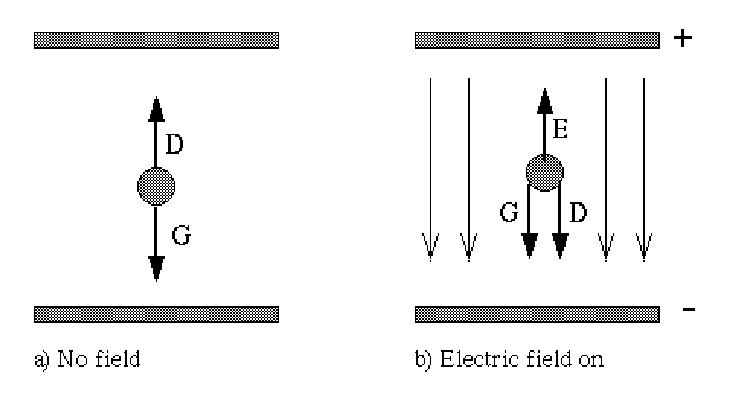
\epsfig{file=Introduction/oil_droplet.eps, height=5cm}
  \caption{
    Forces on an oil-droplet in: \newline
    \hspace*{1.5cm}
           a) Free fall          \newline
    \hspace*{1.5cm}
	   b) Electric field     \newline
    (G=Gravitation, D=Drag, E=Electric force)
  }
  \label{oil_droplet}
\end{center}
\end{figure}

His results were systematically low by about 4\% due to inaccurate
knowledge of the coefficient of viscosity. \newline
The electron charge is -e,
where $e = 1.602 \cdot 10^{-19}C$. All free particles are observed to
have values of electric charge equal to an integer times the
fundamental charge e:

\begin{equation*}
  q=n e
\end{equation*}

where the integer $n=\dots,-1,0,1,\dots$ is the electric charge
\emph{quantum number}.

\subsection*{The Nucleus}

In 1912, Ernest Rutherford and his associates discovered that the
positive charge of the atom is concentrated in a \emph{nucleus}. The
charge of the $\alpha$ particle, discovered by Becquerel, was
determined to be $2e$, and the mass of the $\alpha$ particle was
determined to be about four times the mass of the hydrogen
atom. \newline
A new particle with zero electric charge was discovered by bombarding
beryllium atoms with $\alpha$ particles. James Chadwick showed that
the new particle, the \emph{neutron}, had mass nearly equal to that of
the \emph{proton}.

\subsection*{The Bohr Model of the Atom}

In 1913, Niels Bohr made the first qunatitatively successful model of
the atom. Inspired by the work of Rutherford, Bohr made a planetary
model of the atom; with electrons moving in circular orbits about the
nucleus. This model may seem quite simple in retrospect, but for the
time it was a great advancement of science. In addition to the
classical circular orbits, the second part of Bohr's atomic model
contains a bold hypothesis of new physics. The new physics recognizes
that \emph{angular momentum} is \emph{quantized}; it can take only
certain values:

\begin{equation*}
  L = mvr = n \hbar
\end{equation*}

where $n$ is a positive integer. Solving the energy equations result
in orbits of radius:

\begin{equation*}
  r_n = \frac{n^2\hbar^2}{mke^2}
\end{equation*}

where the \emph{Bohr radius}

\begin{equation*}
  a_0 \equiv r_1 = \frac{\hbar^2}{mke^2} \approx 0.053 nm
\end{equation*}

is in the correct order of magnitude for the size of the atom!

{\bf Planc }

 % introduction.tex
\clearemptydoublepage
%\part{Theoretical Foundations}
%%%%%%%%%%%%%%%%%%%%%%%%%%%%%%%%%%%%%%%%%%%%%%%%%%%%%%%%%%%%%%%%%%%%%%%%%%%%%%%%%%%%%%%%%%%%%%%%%%%%%%%
\chapter{Quantum Mechanics of Many-Body Systems}
\label{ch: Quantum Mechanics of Many-Body Systems}
%%%%%%%%%%%%%%%%%%%%%%%%%%%%%%%%%%%%%%%%%%%%%%%%%%%%%%%%%%%%%%%%%%%%%%%%%%%%%%%%%%%%%%%%%%%%%%%%%%%%%%%

One-particle quantum mechanics deals with systems consisting of only $\textit{one}$ particle. This is of course a natural and necessary starting point for all quantum mechanical considerations, where fundamental postualtes, formalism, quantization effects etc. can be introduced and discussed in piece and quiet without considering implications of real life systems. When this done, it is natural to move over to real physical systems which consists of more than one particle. These systems are often called many-body or many-particle systems in the litterature and provide a breeding ground for many-body theory and dusins of approximation schemes and methods. 

In this chapter, basic quantum mechanics of many-body systems are presented with an emphasize on the apparent everlasting many-body problem. 

%------------------------------------------------------------------------------------------------------
\section{The many-body problem}
\label{sec: the many-body problem}
%------------------------------------------------------------------------------------------------------
We consider an isolated system of $N$ identical particles that we assume can be treated non-relativistic. The properties of the system are given by the fundamental Schr�dinger equation,
\begin{align}
\label{eq:Many-body timedependent Schr�dinger equation}
i\hbar \frac{\partial}{\partial t}\ket{\Psi} = \OP{H}\ket{\Psi},
\end{align}
where $\ket{\Psi}$ is the $N$-particle wave function and $\OP{H}$ is the hamiltonian of the system defined as
\begin{align}
\label{exp:general hamilton operator}
\OP{H} = \OP{T} + \OP{V}.
\end{align}
The operators $\OP{T}$ and $\OP{V}$ denotes the kinetic energy and potential energy of the system, respectively. The time dependent Schr�dinger equation (\ref{eq:Many-body timedependent Schr�dinger equation}) provides all the properties of the system including the time evolution. It is appropriate to introduce the time elvolution operator $\OP{\mathcal{U}}$, which acting on a system state $\ket{\Psi(t_0)}$ yields the time evolution of the system at all times $t>t_0$,
\begin{align}
\label{exp:time evolution operator}
\ket{\Psi(t)} = \OP{\mathcal{U}}(t,t_0)\ket{\Psi(t_0)}.
\end{align}
Inserting (\ref{exp:time evolution operator}) into Eq.(\ref{eq:Many-body timedependent Schr�dinger equation}) yields the equation for the time-evolution operator,
\begin{align}
\label{eq:time evolution operator equation}
i\hbar\frac{\partial}{\partial t}\OP{\mathcal{U}}(t,t_0) = \OP{H}\OP{\mathcal{U}}(t,t_0).
\end{align}
When the hamiltonian is time independent, the time evolution operator reads
\begin{align}
\label{exp:time evolution operator 2}
\OP{\mathcal{U}}(t,t_0) = e^{-\frac{i}{\hbar}\OP{H}(t-t_0)}.
\end{align}
If we were to prepare a system in state $\ket{\Psi(t_0)}$ at time $t_0$, which for convenience often is chosen as $t_0=0$, the system state $\ket{\Psi(t)}$ for all $t>t_0$ is determined by simply letting the time evolution operator act on the initial state. It is already clear that the hamiltonian of the system determine the time evolution of the system, which in itself is a fundamental improtance, but it also provide the energy spectrum and eigenstates which are often our main interest. For example, an analytical expression of Eq. (\ref{exp:time evolution operator 2}) is only possible if the reference state is written as a linear combination of energy eigenstates. 

As pointed out before, the energy eigenvalues and eigenstates are of fundamental importance for every quantum mechanical considerations. When the hamiltonian of the system is stationary, the Schr�dringer equation (\ref{eq:Many-body timedependent Schr�dinger equation}) can be separated in time $t$ and coordinates of chosen representation (basis). This leads to the time-independent Schr�dinger (energy eigenvalue) equation
\begin{align}
\label{eq:Many-body timeindepundendent Schr�dinger equation}
\OP{H}\ket{\Psi_\lambda} = E_\lambda \ket{\Psi_\lambda},
\end{align}
where $\ket{\Psi_\lambda}$ is the energy eigenstate with corresponding eigenvalue $E_\lambda$ and $\lambda$ denote the set of quantum numbers needed for unique specification of the eigenstates. Up to now, no representation (basis) in the Hilbertroom has been chosen, and the previous discussion is valid for any favourite representation. We will in the following apply the coordinate representation, which is the most appropriate choice in the follwing treatment of the many-body problem. The Schr�dinger equation (\ref{eq:Many-body timeindependent Schr�dinger equation}) then reads
\begin{align}
\label{eq:Many-body timeindependent Schr�dinger equation coordinate representation}
\OP{H}(\vek{r}_1,\vek{r}_2,..,\vek{r}_N)\Psi_{\lambda}(\vek{r}_1,\vek{r}_2,..,\vek{r}_N) = E_\lambda \Psi_{\lambda}(\vek{r}_1,\vek{r}_2,..,\vek{r}_N),
\end{align}
where $\vek{r}_i$ are the spatial coordinates, with spin variables included, for the $i$'th particle. The hamiltonian is general, as pointed out before, the sum of the total kinetic energy and potential energy. The kinetic energy operator reads
\begin{align}
\label{exp:Kinetic energy operator}
\OP{T} &= \sum_{i=1}^N \OP{t}(\vek{r}_i) \\
       &= -\frac{\hbar^2}{2m}\sum_{i=1}^N \nabla_i^2.
\end{align}
In the general case, the potential energy operator is build up of $n$-body operators ($n = 1,2,..,N$), and is defined as an operator acting on $n$-particles. For example, the well-known coulomb interaction is a two-body interaction since it depends on the distance between two particles. The potential energy operator thus reads
\begin{align}
\label{exp:Potential energy operator}
 \OP{V} &= \OP{V}_1 + \OP{V}_2 + ... + \OP{V}_N\\
&= \sum_{i=1}^N \OP{v}_1(\vek{x}_i) + \sum_{i<j}^N \OP{v}_2(\vek{x}_i,\vek{x}_j) + ... + \sum_{i<j<..<l}^N \! \OP{v}_N(\vek{x}_i,\vek{x}_j,..,\vek{x}_l),
\end{align}
where the $\vek{x}_i$ is written instead of $\vek{r_i}$ to underline the fact that the potential in the general case also can be a function of for example momentum. In nuclear physics, it is normal to introduce two-body potential operators that is dependent on both spatial position and momentum. The fundamental strong interaction, which keep the nuclei tougether, also seems to exhibit three-body behaviour. This is fundamentally due to the fact that the interaction's exchange particles, called gluons, can couple to themselves. Relevant operators in real many-body systems involve not more than three-body operators, and is therefore usually omitted in the definition of the potential energy operator. For theoretical reasons, all $n$-body operators up are included in the general definition in (\ref{exp:Potential energy operator}).  

The eigenvalue equation in Eq. (\ref{eq:Many-body timeindependent Schr�dinger equation coordinate representation}), with the kinetic energy and potential energy operator defined in Eq. (\ref{exp:Kinetic energy operator}) and Eq.(\ref{exp:Potential energy operator}), respectively, is usually called the $\textit{quantum mechanical many-body}$ $\textit{problem}$. This is a highly non-trivial problem due to the interaction operators. In real-life systems, particles interact with each other, and one would at least have to include two-body operators in the potential energy. Even by only including the two-body interaction $\OP{v}_2$, the many-body problem cannot be solved exactly. In quantum mechanical treatment of many-body systems we are therefore forced to make use of different approxmation schemes and complex techniques. However, the natural starting point for all considerations of many-body systems is, despite the choice of method, the non-interacting system. 

%-------------------------------------------------------------------------------------------------------------------------------------------------------
\section{The non-interacting system}
\label{sec: the non-interacting system}
%-------------------------------------------------------------------------------------------------------------------------------------------------------
The general non-interacting (unperturbed) system consists of $N$ non-interacting particles subject to an external potential $u$. The hamiltonian reads
\begin{align}
\label{exp:Non-interacting hamiltonian}
\OP{H}_0 = \sum_{i=1}^N \OP{h}_0 = -\frac{\hbar^2}{2m}\sum_{i=1}^N \nabla_i^2 + \sum_{i=1}^N u(\vek{r}_i),
\end{align}
where the potential is assumed to be a function of spatial coordinates $\vek{r}_i$ including spin variable. The non-interacting Schr�dinger equation
\begin{align}
\label{eq:Non-interacting schr�dinger equation}
\OP{H}_0\Phi_a(\vek{r}_1,\vek{r}_2,..,\vek{r}_N) = E_a^0 \Phi_a(\vek{r}_1,\vek{r}_2,..,\vek{r}_N),
\end{align}
can be solved exactly by seperation of variables since the hamiltonian only consists of one-body operators. Inserting
\begin{align}
\label{exp:Non-interacting energy eigenvectors}
\Phi_a(\vek{r}_1,\vek{r}_2,..,\vek{r}_N) = \phi_\alpha(\vek{r}_1)\phi_\beta(\vek{r}_2)..\phi_\gamma(\vek{r}_N)
\end{align}
into Eq. (\ref{eq:Non-interacting schr�dinger equation}) yields $N$ identical single-particle equations, 
\begin{align}
\label{eq:Single-particle Schr�dinger equation}
\OP{h}_0 \phi(\vek{r}) = \epsilon \phi(\vek{r}).
\end{align}
We identify Eq. (\ref{eq:Single-particle Schr�dinger equation}) as the Schr�dinger equation for the system when only one particle is present. Solving this equation yields the set of single-particle energy eigenvalues $\kpr{\epsilon}$  and eigenfunctions $\kpr{\phi}$, and hence all the $N$-particle eigenfunctions in Eq. (\ref{exp:Non-interacting energy eigenvectors}) are determined. The total non-interacting energy eigenvalues are found by summing over all the single-particle energies,
\begin{align}
E_a^0 = \sum_{\alpha=1}^N \epsilon_{\alpha}.
\end{align}
A general state in the non-interacting system can be written as the linear combination of energy eigenstates,
\begin{align}
\Phi(\vek{r}_1,\vek{r}_2,..,\vek{r}_N) = \sum_{\kpr{\alpha\beta..\gamma}} c_{\alpha\beta..\gamma} \phi_\alpha(\vek{r}_1)\phi_\beta(\vek{r}_2)..\phi_\gamma(\vek{r}_N),
\end{align}
where $c_{\alpha\beta..\gamma}$ are the expansion coefficients satisfying the normalization condition
\begin{align}
\sum_{\kpr{\alpha\beta..\gamma}} \abs{c_{\alpha\beta..\gamma}}^2 = 1. 
\end{align}

The simple product form of the eigenfunctions in Eq. (\ref{exp:Non-interacting energy eigenvectors}) assumes that we can tell the particles apart. It would otherwise make no sense to claim that particle $1$ is in state $\phi_\alpha$, particle $2$ is in state $\phi_\beta$, and so on. In the classical regime, we can in principle always distinguish particles from each other, but in quantum mechanics, the situation is fundamentally different. When for example considering a system of electrons, we will never be able to tell them apart. Actually, it is not just that we do not happen to know; there is no such thing as ``this'' or ``that'' electron. Electrons are in fact $\textit{utually identical}$ in a way classical objects will never be. This is a feature which has to be baked into the wave function and which gives rise to two types of particles: fermions and bosons. 

%----------------------------------------------------------------------------------------------------------------------------------------------------------
\section{Identical particles}
\label{sec: identical particles}
%----------------------------------------------------------------------------------------------------------------------------------------------------------
The nature of identical particles gives rise to anti-symetric and symetric wave functions. A natural starting point is to investigate the permutation operator $\OP{P}$ and permutation symetri properties of the hamiltonian. The permutation operator $\OP{P}_{12}$ is defined by
\begin{align}
\label{exp:Permutation operator}
\OP{P}_{12} \phi_\alpha (\vek{r}_1)\phi_\beta (\vek{r}_2) = \phi_\alpha (\vek{r}_2) \phi_\beta (\vek{r}_1). 
\end{align}
In words, the permutation operator $\OP{P}_{ij}$ interchange the coordinates of particles $i$ and $j$. In quantum mechanics, the absolute squared of the wave function is interpreted as a probability density. Interchanging the coordinates of two completely identical particles should conserve this quantity, hence
\begin{align}
\abs{\Phi(..,\vek{r}_i,..,\vek{r}_j,..)}^2 = \abs{\Phi(..,\vek{r}_j,..,\vek{r}_i,..)}^2.
\end{align}
Mathematical this imply that 
\begin{align}
\Phi(..,\vek{r}_i,..,\vek{r}_j,..) = \pm \Phi(..,\vek{r}_j,..,\vek{r}_i,..),
\end{align}
which means that the total wave function is either symetric or anti-symetric with respect to the interchange of two particles. This is also shown by investigating the permutation operator and the hamiltonian. The hamiltonian for a system of identical particles is invariant under the interchange of particle coordinates. This imply that
\begin{align}
\fpr{\OP{H_0},\OP{P}_{ik}} = 0,
\end{align}
and hence we are in a position to construct eigenfunctions $\Phi_a$ of $\OP{H}_0$ that are also eigenfunctions of $\OP{P}_{ij}$ (see \cite{Dickhoff}). The eigenvalue equation of the permutation operator reads
\begin{align}
\OP{P}_{ij}\Phi_a(\vek{r}_1,..,\vek{r}_i,..,\vek{r}_j,..,\vek{r}_N) = \beta \Phi_a(\vek{r}_1,..,\vek{r}_j,..,\vek{r}_i,..,\vek{r}_N),
\end{align}
and the fact that 
\begin{align}
\label{exp:Permutation operator 2}
\OP{P}_{ij}^2 = 1,
\end{align}
implies that 
\begin{align}
\label{exp:Permutation operator 3}
\beta = \pm 1.
\end{align}
The pluss sign denotes systems of identical $\textit{bosons}$ where the wave function is symetric under the interchange of two particles. The minus sign denotes systems of $\textit{fermions}$ where the wave function is anti-symtetric under the interchange of two particles. Depending of whether the system consists of identical bosons or fermions, the eigenfunctions of Eq. (\ref{eq:Non-interacting schr�dinger equation}) must be either symetric or anti-symetric. Considering a two-particle system, the symetric and anti-symetric wave function reads
\begin{align}
\Phi_{+}(\vek{r}_1, \vek{r}_2) &= \frac{1}{\sqrt{2}}\fpr{\phi_\alpha(\vek{r}_1)\phi_\beta(\vek{r}_2) + \phi_\alpha(\vek{r}_2)\phi_\beta(\vek{r}_1)},\\
\Phi_{-}(\vek{r}_1, \vek{r}_2) &= \frac{1}{\sqrt{2}}\fpr{\phi_\alpha(\vek{r}_1)\phi_\beta(\vek{r}_2) - \phi_\alpha(\vek{r}_2)\phi_\beta(\vek{r}_1)}.
\end{align}
These states are eigenstates of the permutation operator $\OP{P}$ with eigenvalue $+1$ and $-1$, respectively. In addition they are also eigenstates of the non-interacting hamiltonian $\OP{H}_0$, both with energy eigenvalue
\begin{align}
E_0 = \epsilon_\alpha + \epsilon_\beta.
\end{align}
In the general case, a symetric and anti-symetric wave function for the $N$-patricle system can be generated by a symetrizer and antisymetrizer operator, respectively, by acting on the product state in Eq. (\ref{exp:Non-interacting energy eigenvectors}). The symetrizer is defined as
\begin{align}
\label{exp:Antisymmetrizer operator}
\OP{\mathcal{A}} = \frac{1}{\sqrt{N!}}\sum_p (-1)^p \OP{P}_p,
\end{align}
and the antisymetrizer as
\begin{align}
\label{exp:Symmetrizer operator}
\OP{\mathcal{S}} = \frac{1}{\sqrt{N!}}\sum_p \OP{P}_p.
\end{align}
A symetric and antisymetric $N$-particle wave function is then generated by letting these operators act on the product states,
\begin{align}
\label{exp:Symmetrized energy eigenfunctions}
\Phi_S(\vek{r}_1,\vek{r}_2,..,\vek{r}_N) &=  \frac{1}{\sqrt{n_\alpha!n_\beta!..n_\gamma!}}\OP{\mathcal{S}} \phi_\alpha(\vek{r}_1) \phi_\beta(\vek{r}_2)..\phi_\gamma(\vek{r}_N)\\
\label{exp:Antisymetrized energy eigenfunctions}
\Phi_{AS}(\vek{r}_1,\vek{r}_2,..,\vek{r}_N) &= \OP{\mathcal{A}} \phi_\alpha(\vek{r}_1) \phi_\beta(\vek{r}_2)..\phi_\gamma(\vek{r}_N).
\end{align}
An important feature of the fermionic antisymetric wave function is that every single-particle state $\phi_\alpha$ can only be occupied by $\textit{one}$ electron only. If we were to put two fermions in the same single-particle state, the wave function would simply be equal to zero, which is completely nonsense. This is the famous Pauli exclusion principle. The bosonic symetric wave function, on the other hand, has no occupancy limit within each single-particle wave function. Bosons and fermions manifest themselves in the nature as $\textit{integer}$ and $\textit{half integer}$ spin particles, respectively. In relativistic quantum mechanics, this feature can actually be proved. We refer to standard textbooks in relativistic quantum field theory.

In general, a system of bosons and a system of fermions manifest quite different properties due to the symetric and antisymetric wave functions. For example, identical bosons tend to be somewhat closer together, and identical fermions somewhat farther apart, than distinguishable particles in the same single-particle states. This can be shown explicit by calculating the two-particle system expectation value $\forv{(x_1 - x_2)^2}$ (coordinates $1$-dimension). After some tedious algebra (see \cite{Griffiths}), the bosonic/fermionic expectation value reads
\begin{align}
\forv{(x_1-x_2)^2}_\pm = \forv{(x_1-x_2)^2} \mp 2\abs{\forv{x}_{\alpha\beta}}^2, 
\end{align}
where $\forv{(x_1-x_2)^2}$ denote the expectation (reference) value for distinguishable particles, and
\begin{align}
\forv{x}_{\alpha \beta} = \int \! x \phi_\alpha^\ast(x)\phi_\beta(x)dx.
\end{align}
When the single-particle wave functions overlap, the system behaves as though there were an attraction force between identical bosons, and a repulsion force between identical fermions. In the literature, this is called the exchange force. It is important to note that this is not a real force, but merely a geometrical consequence of the wave function symetrization.

We have till now omitted the spin in our discussion. The $\textit{total}$ non-interacting energy eigenfunctions consist of a spatial part and a spin part, connected together with a tensor product,
\begin{align}
\Phi_{TOT} = \Phi \otimes \chi.
\end{align}
It is the $\textit{total}$ wave function that should obey the symetrization requirements, not just the spatial part. A system of fermions require the spatial part and the spin part to have opposite symetrization, while a system of bosons require equal symetrization. All expressions till now are still valid by including the spin inside the total single-particle quantum number $\alpha$.

As pointed out before, the basic fundament for all quantum mechanical treatment of interacting many-body systems is the non-interacting system, which is the natural first approximation. Important features of the full wave function and the hamiltonian can be extracted, giving essential and fundamental information of system from the very start, both in the sense of physical reality and numerical expenditure. In the next section, the treatment of many-body systems with interacting particles is presented. 

%----------------------------------------------------------------------------------------------------------------------------------------------------------
\section{The interacting many-body system}
\label{sec: the interacting many-body system}
%----------------------------------------------------------------------------------------------------------------------------------------------------------
In this section, the interacting many-body system is considered. We will limit the discussion to fermionic systems with antisymetric wave function. The Schr�dinger equation reads
\begin{align}
\OP{H}\Psi_\lambda(\vek{r}_1,\vek{r}_2,..,\vek{r}_N) = E_\lambda\Psi_\lambda(\vek{r}_1,\vek{r}_2,..,\vek{r}_N).
\end{align}
As pointed out before, this equation cannot, in general, be solved exactly for $N>1$. Nevertheless, general properties of the wave function $\Psi_\lambda$ can be determined by looking at the symmetry of the hamiltonian $\OP{H}$. For example, letting $\OP{H}$ be rotational invariant, i.e. 
\begin{align}
\fpr{\OP{H},\OP{R}} = 0,
\end{align}
where $\OP{R}$ is the intrinsic spin rotation operator, the total spin of the system is said to be conserved. This means that acting with $\OP{H}$ on $\textit{any}$ $N$-particle wave function $\ket{f} \in \mathcal{H}_N$ with spin $s_f$,
\begin{align}
\OP{H}\ket{f} = \ket{g},
\end{align}
yield a $N$-particle function $\ket{g} \in \mathcal{H}_N$ with the same spin. This allow us to diagonalize the hamiltonian seperate for each total spin, so that we obtain reduction of the matrix dimensionality.  
\begin{tikzpicture}
\draw (0,0) -- (2,0);
\draw (2,0) -- (2,2);
\draw (2,2) -- (0,2);
\draw (0,2) -- (0,0);
\draw (3,0) -- (5,0);
\draw (5,0) -- (5,2);
\draw (5,2) -- (3,2);
\draw (3,2) -- (3,0);
%(1,1) circle (2pt)
%(2,1) circle (2pt)
%(2,0) circle (2pt);
%\draw (0,0) .. controls (1,1) and (2,1) .. (2,0);
\end{tikzpicture}

An other important symmetry property of the hamiltonian is the permutation symmetry. In the previous section, the permutation operator was defined in Eq. (\ref{exp:Permutation operator}). The full interacting hamiltonian for a system of identical particles are invariant under the permutation of particle coordinates, i.e.
\begin{align}
\fpr{\OP{H},\OP{P}} = 0. 
\end{align}
Hence we can construct a set of functions $\kpr{\Psi}$ that are eigenfunctions of both $\OP{H}$ and $\OP{P}$. The eigenvalue equation for the permutation operator reads
\begin{align}
\OP{P}_{ij}\Psi_\lambda(\vek{r}_1,..,\vek{r}_i,..,\vek{r}_j,..,\vek{r}_N) = \beta \Psi_\lambda(\vek{r}_1,..,\vek{r}_i,..,\vek{r}_j,..,\vek{r}_N).
\end{align}
Since Eq. (\ref{exp:Permutation operator 2}) and Eq. (\ref{exp:Permutation operator 3}) still holds, the total wave function $\Psi_\lambda$ is either symetric or antisymetric depending on whether the system consits of bosons or fermions. 

%----------------------------------------------------------
\subsection{Hilbert spaces of distinguishable particles}
\label{subsec: hilbert spaces of distinguishable particles}
%----------------------------------------------------------
Consider a system of $N$ distinguishable particles. The $\textit{total wave function}$ lives in the infinite $N$-particle Hilbert space $\mathcal{H}_N$. Assume we have found a one-particle infinite basis set $\mathcal{B}_1^\alpha = \kpr{\ket{\alpha}}$ which span the $1$-particle hilbertspace $\mathcal{H}_1$. The quantum number $\alpha$ can correspond to position, momentum or your favourite basis functions that fullfill the orthonormality relation and completeness relation. The $N$-particle Hilbert space can be constructed by building it out of $N$ one-particle spaces,
\begin{align}
\mathcal{H}_N = \mathcal{H}_{1_1 \otimes 1_2 \otimes ... \otimes 1_N} = \mathcal{H}_{1_1} \otimes \mathcal{H}_{1_2} \otimes ... \otimes \mathcal{H}_{1_N},  
\end{align}
which is called the $\textit{direct product space}$. $\OP{H}_{1_i}$ denote the $1$-particle Hilbert space for particle $i$. The basis set of the $N$-particle product space can be constructed in a similar fashion,
\begin{align}
\label{exp:Direct product states}
\ket{\alpha \beta .. \gamma} = \ket{\alpha} \otimes \ket{\beta} \otimes .. \otimes \ket{\gamma},
\end{align}
which is often refered to as the $\textit{direct product basis}$. See \cite{Shankar} for a complete discussion. When considering a system of $N$ distinguishable particles, the total wave function can be written as a linear combination of the product states,
\begin{align}
\ket{\Psi_D} = \sum_{\kpr{\alpha\beta..\gamma}} c_{\alpha\beta..\gamma}\ket{\alpha\beta..\gamma}.
\end{align}
In the coordinate representation, the wave function then reads
\begin{align}
\label{exp:Distinguishable particles 1}
\Psi_D(\vek{r}_1,\vek{r}_2,..,\vek{r}_N) =  \sum_{\kpr{\alpha\beta..\gamma}} c_{\alpha\beta..\gamma}\phi_\alpha(\vek{r}_1)\phi_\beta(\vek{r}_2)..\phi_\gamma(\vek{r}_N).
\end{align}
In Eq. (\ref{exp:Distinguishable particles 1}), the single-particle basis functions are written as $\phi$ (see section \ref{sec: The non-interacting system}) to underline the fact that the $\textit{natural}$ and $\textit{good}$ basis functions are in most cases those generated from the non-interacting system. Nevertheless, Eq. (\ref{exp:Distinguishable particles 1}) are valid for $\textit{any}$ single-particle basis set.

%---------------------------------------------------
\subsection{Bosonic and fermionic Hilbert spaces}
\label{subsec: bosonic and fermionic hilbert spaces}
%---------------------------------------------------
Consider a system of $N$ bosonic or fermionic particles. As pointed out before, the total $N$-particle wave function must satisfy symetrization requirements. We denote the $N$-particle Hilbert space of symmetric bosonic vectors $\mathcal{H}^S_N$ and the Hilbert space of antisymmetric fermionic vectors $\mathcal{H}^{A}_N$. In the two-particle system, to each pair of product states $\ket{\alpha\beta}$ and $\ket{\beta \alpha}$, there exist one symmetric bosonic vector and one antisymmetric fermionic vector. When $\alpha = \beta$, the product state is already symmetric, and a fermionic state does not exist due to Pauli exclusion principle. The two-particle Hilbert space has thus enough basis states to form one symmetric space and one antisymmetric space, written as
\begin{align}
\mathcal{H}_2 = \mathcal{H}^S_2 \oplus \mathcal{H}^A_2,
\end{align}
and in the general $N$-particle case,
\begin{align}
\mathcal{H}_N = \mathcal{H}^S_N \oplus \mathcal{H}^A_N.
\end{align}
In the literature, one often view $\mathcal{H}^S_N$ and $\mathcal{H}^A_N$ as subspaces of $\mathcal{H}_N$. Given a system of $N$ bosons or fermions, the state will be an element of $\mathcal{H}_N^S$ or $\mathcal{H}_N^A$, respectively. It can also be shown that a system that initially starts out in the symmetric or antisymmetrix subspace, will remain in the same subspace for all later times. Hence, by considering a system of bosons (fermions) it is sufficient to only deal with the symmetric (antisymmetric) subspace.

The basis functions for the symmetric $N$-particle Hilbert space and the antisymmetric $N$-particle Hilbert space can be constructed from an orthonormal and colomplete single-particle basis set. As was the case for distinguishable particles, the direct product states in Eq. (\ref{exp:Direct product states}) do not constitute a basis for the symmetric and antisymmetric subspaces. As can be done for all wave functions, the bosonic and fermionic states can be written as a linear combination of a (at the moment unknown) basis set,
\begin{align}
\ket{\Psi_B} &= \sum_i c_i \ket{i}\\
\ket{\Psi_F} &= \sum_j c_j \ket{j}.
\end{align}
To have $\ket{\Psi_S}$ and $\ket{\Psi_A}$ symmetric and antisymmetric, respectively, require the basis functions $\ket{i}$ to be symmetric and $\ket{j}$ to be antisymmetric. Since the product states are not all symmetric and antisymmetric, they cannot be used as basis functions. In section \ref{sec: Identical particles}, symmetric and antisymmetric states were constructed from the product states, see Eq. (\ref{exp:Symmetrized energy eigenfunctions}) and Eq. (\ref{exp:Antisymetrized energy eigenfunctions}). $\textit{These}$ functions have the correct symmetry in addition to inherit the orthonormality from the product states. Hence, 
\begin{align}
\ket{i} &=  \frac{1}{\sqrt{n_\alpha!n_\beta!..n_\gamma!}}\OP{\mathcal{S}} \ket{\alpha\beta..\gamma}\\
\ket{j} &= \OP{\mathcal{A}} \phi_\alpha(\vek{r}_1) \ket{\alpha\beta..\gamma},
\end{align}
where the symmetrizer operators are defined in Eq. (\ref{exp:Symmetrizer operator}) and Eq. (\ref{exp:Antisymmetrizer operator}). $\textit{Any}$ orthonormal and complete single-particle basis can be used. Nevertheless, as was the case for distinguishable particles, the $\textit{good}$ single-particle basis is often the non-interacting set. Written in the coordinate representation, the bosonic and fermionic wave function reads
\begin{align}
\Psi_B(\vek{r}_1,\vek{r}_2,..,\vek{r}_N) &=  \sum_{\kpr{\alpha\beta..\gamma}} \frac{c_{\alpha\beta..\gamma}}{\sqrt{n_\alpha!n_\beta!..n_\gamma!}}\OP{\mathcal{S}} \phi_\alpha(\vek{r}_1) \phi_\beta(\vek{r}_2)..\phi_\gamma(\vek{r}_N)\\
\label{exp:Fermionic wave function}
\Psi_{F}(\vek{r}_1,\vek{r}_2,..,\vek{r}_N) &= \sum_{\kpr{\alpha\beta..\gamma}} d_{\alpha\beta..\gamma}\OP{\mathcal{A}} \phi_\alpha(\vek{r}_1) \phi_\beta(\vek{r}_2)..\phi_\gamma(\vek{r}_N).
\end{align}
The fermionic basis functions in Eq. (\ref{exp:Fermionic wave function}) can be written as a determinant, called $\textit{Slater determinant}$,
\begin{align}
\label{exp: Slater determinant}
\Phi_{\alpha\beta..\gamma}(\vek{r}_1,\vek{r}_2,..,\vek{r}_N) = \frac{1}{\sqrt{N!}}\left|\begin{array}{cccc}\phi_\alpha(\vek{r}_1) & \phi_\beta(\vek{r}_1) & \cdots & \phi_\gamma(\vek{r}_1)\\
\phi_\alpha(\vek{r}_2) & \phi_\beta(\vek{r}_2) & \cdots & \phi_\gamma(\vek{r}_2) \\ \vdots & \vdots & \vdots & \vdots\\ 
\phi_\alpha(\vek{r}_N) & \phi_\beta(\vek{r}_N) & \cdots & \phi_\gamma(\vek{r}_N)\end{array} \right|,
\end{align}
where $\Phi$ and $\phi$ are used to indicate that we are working with the good basis, i.e. the non-interacting set. But as pointed out before, every set of single-particle functions satisfying basis requirements, can be used. A general fermionic wave function can thus be expanded as an infinite series of Slater determinants,
\begin{align}
\Psi_{F}(\vek{r}_1,\vek{r}_2,..,\vek{r}_N) &= \sum_{\kpr{\alpha\beta..\gamma}} d_{\alpha\beta..\gamma} \Phi_{\alpha\beta..\gamma}(\vek{r}_1,\vek{r}_2,..,\vek{r}_N).
\end{align}

%-------------------------------------------------------------------------------------------------------------------------------------------------------
\section{Correlations in many-body systems}
\label{sec: correlations in many-body systems}
%-------------------------------------------------------------------------------------------------------------------------------------------------------

%-------------------------------
\section{Second Quantization}
\label{sec: Second Quantization}
%-------------------------------
In the previous section, the so-called slater determinant was introduced. Eq. (\ref{exp: Slater determinant}) clearly shows by construction that one may never assign one-to-one correspondence between single-particle states and particle coordinates, which is a direct consequence of the particles identical nature. The only thing we can say is what single-particle orbital is occupied. Thus the full slater determinant in Eq. (\ref{exp: Slater determinant}) include much redundant information, and it is therefore appropriate to characterize slater determinants by single-particle states only. Hence we write the slater determinant in Eq. (\ref{exp: Slater determinant}) in the more abstract, yet simpler, form
\begin{align}
\Phi_{\alpha_1\alpha_2..\alpha_N} \equiv \ket{\alpha_1\alpha_2..\alpha_N}.
\end{align}
This notation is called the occupancy representation, for the obvious reason. This form of the antisymmetrized wave function does not explicit reflect the antisymmetry in the particle coordinates. Nevertheless, the slater determinant changes sign in permutation of two columns, so that the abstract notation also is antisymmetric to permutation of single-particle orbitals,
\begin{align}
\label{exp: Slater determinant antisymmetry}
\ket{\alpha_1..\alpha_i..\alpha_j..\alpha_N} = -\ket{\alpha_1..\alpha_i..\alpha_j..\alpha_N}.
\end{align}
The full potential of the occupancy notation for antisymmetrized states is released when creation and annihilation operators is introduced. Creation operators create fermions in single-particle states, while the annihilation operators remove fermions from single-particle states. In many-body theory literature, this formalism is called second quantization, even though it has not the direct physical interpretation as in relativistic quantum field theory, where the second quantization originally was introduced. In the field theory, this formalism reflects physical processes such as creation and annihilation of quanta. In the non-relativistic quantum field theory, the formalism of creation and annihilation operators is intruduced for appropriate reasons. For example, the second quantization formalism allow us to use the pratical particle-hole formalism. 

%--------------------------------------------------
\subsection{Creation and annihilation operators}
\label{subsec: Creation and annihilation operators}
%--------------------------------------------------
The creation and annihilation operators are defined as operators that create and annihilate particles in single-particle states. We define the fermionic creation operator $\cre{\alpha}$ as
\begin{align}
\label{exp: Creation operator 1}
\cre{\alpha}\ket{0} &\equiv \ket{\alpha}\\
\label{exp: Creation operator 2}
\cre{\alpha}\ket{\alpha_1\alpha_2..\alpha_N} &\equiv \ket{\alpha\alpha_1\alpha_2..\alpha_N}\\
\label{exp: Creation operator 3}
\cre{\alpha}\ket{\alpha_1\alpha_2..\alpha..\alpha_N} &\equiv 0.
\end{align}
In Eq. (\ref{exp: Creation operator 1}), the creation operator acts on the vacuum state, that is the state with no particles, and creates a fermion in state $\alpha$. In Eq. (\ref{exp: Creation operator 2}), the operator acts on the $N$-fermion state with single-particle states $\alpha_i \neq \alpha$, yielding a $N+1$-fermion system where a fermion in state $\alpha$ has been created. When the creation operator acts on the $N$-fermion state in Eq. (\ref{exp: Creation operator 3}) where the single-particle orbital $\alpha$ already is occupied, the result is zero. The definitions above imply that the full slater determinant can be written as a product of creation operators,
\begin{align}
\label{exp: Slater determinant second quantization}
\ket{\alpha_1\alpha_2..\alpha_N} = \cre{\alpha_1}\cre{\alpha_2}..\cre{\alpha_N}\ket{0}.
\end{align}
Combining Eq. (\ref{exp: Slater determinant second quantization}) and Eq. (\ref{exp: Slater determinant antisymmetry}) into 
\begin{align}
\cre{\alpha_1}..\cre{\alpha_i}..\cre{\alpha_j}..\cre{\alpha_N}\ket{0} = -\cre{\alpha_1}..\cre{\alpha_j}..\cre{\alpha_i}..\cre{\alpha_N}\ket{0},
\end{align}
yields the commutation relation
\begin{align}
\label{exp: Creation operator commutation relation}
\kpr{\cre{\alpha},\cre{\beta}} = \cre{\alpha}\cre{\beta} + \cre{\beta}\cre{\alpha} = 0. 
\end{align}
By taking the hermitian conjugate of the creation operator we obtain the operator $\an{{\alpha}} = \pr{\cre{\alpha}}^\dagger$. First of all, the hermitian conjugate of Eq. (\ref{exp: Creation operator commutation relation}) yield the commutation relation
\begin{align}
\label{exp: Annihilation operator commutation relation}
\kpr{\an{{\alpha}},\an{{\beta}}} = \an{{\alpha}}\an{{\beta}} + \an{{\beta}}\an{{\alpha}} = 0. 
\end{align}
The action of $\an{\alpha}$ on a slater determinant reads,
\begin{align}
\label{exp: Annihilation operator 1}
\an{\alpha}\ket{0} &= 0\\
\label{exp: Annihilation operator 2}
\an{\alpha_i}\ket{\alpha_1..\alpha_{i-1}\alpha_i\alpha_{i+1}..\alpha_N} &= (-1)^p\ket{\alpha_i\alpha_1..\alpha_{i-1}\alpha_{i+1}..\alpha_N} = (-1)^p \ket{\alpha_1..\alpha_{i-1}\alpha_{i+1}..\alpha_N}\\
\label{exp: Annihilation operator 3}
\an{\alpha}\ket{\alpha_1\alpha_2..\alpha_N} &= 0.
\end{align}
These realtions follow from the definition of the creation operator in Eq. (\ref{exp: Creation operator 1}), (\ref{exp: Creation operator 2}) and (\ref{exp: Creation operator 3}). We refer to \cite{Dickhoff} for a further discussion. In Eq. (\ref{exp: Annihilation operator 1}), the annihilation operator acts on the vacuum state, yielding zero. In Eq. (\ref{exp: Annihilation operator 2}), the annihilation operator removes a fermion from single-particle state $\alpha_i$. When the $N$-particle state does not include the removal state, which is the case in Eq. (\ref{exp: Annihilation operator 3}), the result is zero. These results clarify why $\an{\alpha}$ is called the fermionic annihilation (destruction) operator. The commutation relation between the creation and annihilation operator (see \cite{Dickhoff}) reads
\begin{align}
\label{exp: Creation and annihilation commutation relation}
\kpr{\cre{\alpha},\an{\beta}} = \delta_{\alpha\beta}.
\end{align}

Since all antisymmetric wave functions are superpositions of slater determinants, we are noe in a position to express these states as products of creation operators acting on the vacuum state. The particle-hole formalism allow us to introduce a new reference state, which can be used to shrink the dimesionality of the problem. Before we discuss this formalism, operators in second quantization is introduced. 

%-----------------------------------------------
\subsection{Operators in second quantization}
\label{subsec: Operators in second quantization}
%-----------------------------------------------
We are now in a position to express many-fermion states by creation and annihilation operators. In many-body theory, however, it almost always comes down to evaluating matrix elements or expectation values of operators. Thus to get full profit of the second quantization formalism we also have to express operators by creation and annihilation operators. Operators expressed in the formalism of second quantization also have the convenient property that they do not depend on the numbers of particles in the system. They work in the so-called Fock space (see \cite{Dickhoff}), which is the vector space constructed by the direct sum of the vacuum space, the single-particle Hilbert space, the two-particle Hilbert space, and so forth, yielding
\begin{align}
\mathcal{F} = \bigoplus_{n=0}^\infty \mathcal{H}^{A}_n. 
\end{align}
This gives us a huge advantage in the way that we for example can work with a given ab initio method, deduce equations, and so forth, without specifying the size of the system. We will in the following only consider the second quantized form of one- en two-body operators. The formalism may be applied to higher order operators, and we refer the reader to any textbook on many-body theory. 

A one-body operator $\OP{F}$ consists of a sum of single-particle operators $\OP{f}$. In an $N$-particle space, the operator reads
\begin{align}
\OP{F} = \sum_{i=1}^N \OP{f}(i),
\end{align}
where $f(i)$ acts on particle $i$ and $N$ is the total number of particles. Given an arbitrary single-particle basis $\kpr{\ket{\alpha}}$, the second quantized formulation of a generic one-body operator $\OP{F}$ (see deduction in \cite{Dickhoff}) reads
\begin{align}
\OP{F} = \sum_{\alpha\beta}\for{\alpha}{f}{\beta}\cre{\alpha}\an{\beta}.
\end{align}
The operator $\OP{F}$ thus annihilates a particle in state $\beta$ and creates a particle in state $\alpha$ with probability amplitude $\for{\alpha}{f}{\beta}$. 

A two-body operator $\OP{V}$ in the $N$-particle space is given by
\begin{align}
\OP{V}_N = \sum_{i<j}^N \OP{v}(i,j),
\end{align}
where $\OP{v}(i,j)$ acts on particle $i$ and $j$, and $N$ is the number of particles in the system. Given an arbitrary two-particle basis product basis $\kpr{\ket{\alpha\beta}}$, the second quantized formulation of a generic two-body operator $\OP{V}$ (see deduction i \cite{Dickhoff}) reads
\begin{align}
\label{exp: Two-body operator second quantization}
\OP{V} &= \frac{1}{2}\sum_{\alpha\beta\gamma\delta}\for{\alpha\beta}{v}{\gamma\delta}\cre{\alpha}\cre{\beta}\an{\delta}\an{\gamma}\\
&= \frac{1}{4}\sum_{\alpha\beta\gamma\delta}\for{\alpha\beta}{v}{\gamma\delta}_{AS}\cre{\alpha}\cre{\beta}\an{\delta}\an{\gamma},
\end{align}
where the antisymmetrized matrix element is defined as
\begin{align}
\for{\alpha\beta}{v}{\gamma\delta}_{AS} = \for{\alpha\beta}{v}{\gamma\delta} - \for{\alpha\beta}{v}{\delta\gamma}.
\end{align}
The operator $\OP{V}$ annihilates a particle from state $\gamma$ and $\delta$, and creates a particle in state $\alpha$ and $\gamma$, with probability amplitude $\frac{1}{4}\for{\alpha\beta}{v}{\gamma\delta}_{AS}$.

We have now established the formalism of second quantization for both antisymmetric wave functions, and one- and two-body operators. As pointed out before, in quantum mechanical many-body calculations, we often end up with evaluating matrix elements. As an example, consider 
\begin{align}
\for{\alpha_1\alpha_2}{\OP{V}}{\alpha_3\alpha_4},
\end{align}
where $\ket{\alpha_1\alpha_2}$ and $\ket{\alpha_3\alpha_4}$ denote slater determinants. We now incorporate the formalism of second quantuzation, with 
\begin{align}
\bra{\alpha_1\alpha_2} &= \bra{0}\an{\alpha_1}\an{\alpha_2}\\
\ket{\alpha_3\alpha_4} &= \cre{\alpha_3}\cre{\alpha_4}\ket{0},
\end{align}
and $\OP{V}$ given by Eq. (\ref{exp: Two-body operator second quantization}). This yields
\begin{align}
\for{\alpha_1\alpha_2}{\OP{V}}{\alpha_3\alpha_4} = \frac{1}{4}\sum_{\alpha\beta\gamma\delta}\for{\alpha\beta}{v}{\gamma\delta}_{AS}\for{0}{\an{\alpha_1}\an{\alpha_2}\cre{\alpha}\cre{\beta}\an{\delta}\an{\gamma}\cre{\alpha_3}\cre{\alpha_4}}{0}. 
\end{align}
Hence we are ending up with evaluating vacuum expectation values of products of creation and annihilation operators. These expressions can be evaluated by using the anticommutation relations in Eq. (\ref{exp: Creation operator commutation relation}), (\ref{exp: Annihilation operator commutation relation}) and (\ref{exp: Creation and annihilation commutation relation}). However, this approach can be quite tedious even for relatively short operator strings, and many opportunities for error may arise. Wick's theorem provides an easy, yet sophisticated, method for writing a string of creation and annihilation operators as a sum of $\textit{normal ordered}$ terms with all possible combinations of $\textit{contractions}$. This allow us to immediately point out which terms that contribute to the matrix element expression. In the next section, Whick's theorem is presented with definitions of normal ordering and contractions.

%-------------------------------
\subsection{Whick's theorem}
\label{subsec: Whick's theorem}
%-------------------------------
Every treatment of the non-relativistic quantum mechanical many-body problem entails calculating matrix elements of operators between state vectors. As pointed out before, in second quantization this imply vacuum expectation values creation and annihilation operator strings. The basic method is to use the anticommuation relations to rearrange the product into an operator string where the annihilation operators stand to the right of the creation operators. All terms with an annihilation operator to the rightmost are zero, by construction. Thus, according to Eq. (\ref{exp: Creation and annihilation commutation relation}), every vacuum expectation value of creation and annihilation operators can be written as a sum of delta-functions. Even though the procedure is straightforward in itself, it becomes tedious and timeconsuming even for expectation values involving only few particles and simple two-body operators. In addition, errors often arise as a natural consequence. We are therefore seeking a method to calculate vacuum expectation values of products of creation and annihilation operators in a simple and systematic way without explicit using the anticommutation relations. Wick's theorem is such a method. 

Wick's theorem is based on two fundamental concepts, namely $\textit{normal ordering}$ and $\textit{contraction}$. The normal-ordered form of $\OP{A}\OP{B}..\OP{X}\OP{Y}$, where the individual terms are either a creation or annihilation operator, is defined as
\begin{align}
\label{def: Normal ordering}
\kpr{\OP{A}\OP{B}..\OP{X}\OP{Y}} \equiv (-1)^p\fpr{\text{creation operators}}\cdot\fpr{\text{annihilation operators}}.
\end{align}
The $p$ subscript denotes the number of permutations that is needed to transform the original string into the normal-ordered form. A contraction between to arbitrary operators $\OP{X}$ and $\OP{Y}$ is defined as  
\begin{align}
\contraction[0.5ex]{}{\OP{A}}{}{\OP{B}}{} 
\OP{A}\OP{B}  \equiv \for{0}{\OP{X}\OP{Y}}{0}.
\end{align}
It is also possible to contract operators inside a normal ordered products. We define the  original relative position between two operators in a normal ordered product as $p$, the so-called permutation number. This is the number of permutations needed to bring one of the two operators next to the other one. A contraction between two operators with $p \neq 0$ inside a normal ordered is defined as
\begin{align}
\kpr{\contraction[0.5ex]{}{\OP{A}}{\OP{B}..}{\OP{X}}\OP{A}\OP{B}..\OP{X}\OP{Y}} = \pr{-1}^p \kpr{\contraction[0.5ex]{}{\OP{A}}{}{\OP{B}}\OP{A}\OP{B}..\OP{X}\OP{Y}}.
\end{align}
In the general case with $m$ contractions, the procedure is similar, and the prefactor changes to 
\begin{align}
\pr{-1}^{p_1 + p_2 + .. + p_m}.
\end{align} 
 
Wick's theorem states that every string of creation and annihilation operators can be written as a sum of normalordered products with all possible ways of contractions,
\begin{align}
\label{def: Wick's theorem}
\OP{A}\OP{B}\OP{C}\OP{D}..\OP{R}\OP{X}\OP{Y}\OP{Z} &= \kpr{\OP{A}\OP{B}\OP{C}\OP{D}..\OP{R}\OP{X}\OP{Y}\OP{Z}}\\
&+ \sum_{\pr{1}} \kpr{ 
\contraction[0.5ex]{}{\OP{A}}{}{\OP{B}} \OP{A}\OP{B}\OP{C}\OP{D}..\OP{R}\OP{X}\OP{Y}\OP{Z}}\\
&+ \sum_{\pr{2}} \kpr{\contraction[0.5ex]{}{\OP{A}}{\OP{B}}{\OP{C}}\contraction[1.0ex]{\OP{A}}{\OP{B}}{\OP{C}}{\OP{D}}\OP{A}\OP{B}\OP{C}\OP{D}..\OP{R}\OP{X}\OP{Y}\OP{Z}}\\
&+ ...\\
&+ \sum_{\fpr{\frac{N}{2}}}\kpr{\contraction[0.5ex]{}{\OP{A}}{\OP{B}}{\OP{C}}\contraction[1.0ex]{\OP{A}}{\OP{B}}{\OP{C}}{\OP{D}} \OP{A}\OP{B}\OP{C}\OP{D}..\contraction[0.5ex]{}{\OP{R}}{\OP{X}}{\OP{Y}}\contraction[1.0ex]{\OP{R}}{\OP{X}}{\OP{Y}}{\OP{Z}}\ \OP{R}\OP{X}\OP{Y}\OP{Z}}.
\end{align}
The $\sum_{\pr{m}}$ means the sum over all terms with $m$ contractions, while $\fpr{\frac{N}{2}}$ means the largest integer that not do not exceeds $\frac{N}{2}$ where $N$ is the number of creation and annihilation operators. When $N$ is even, 
\begin{align}
\label{exp: Wick condition}
\fpr{\frac{N}{2}} = \frac{N}{2},
\end{align}
and the last sum in Eq. (\ref{def: Wick's theorem}) is over fully contracted terms. When $N$ is odd,
\begin{align}
\fpr{\frac{N}{2}} \neq \frac{N}{2},
\end{align}
and non of the terms in Eq. (\ref{def: Wick's theorem}) are fully contracted. Whe refer to \cite{Dickhoff} for a complete proof of Wick's theorem. 

An important extension of Wick's theorem allow us to define contractions between normal-ordered strings of operators. This is the so-called generalized Wick's theorem,
\begin{align}
\label{def: Generalized Wick's theorem}
\kpr{\OP{A}\OP{B}\OP{C}\OP{D}..}\kpr{\OP{R}\OP{X}\OP{Y}\OP{Z}..} &= \kpr{\OP{A}\OP{B}\OP{C}\OP{D}..\OP{R}\OP{X}\OP{Y}\OP{Z}}\\
&+ \sum_{\pr{1}} \kpr{ 
\contraction[0.5ex]{}{\OP{A}}{\OP{B}\OP{C}\OP{D}..}{\OP{R}} \OP{A}\OP{B}\OP{C}\OP{D}..\OP{R}\OP{X}\OP{Y}\OP{Z}}\\
&+ \sum_{\pr{2}} \kpr{\contraction[0.5ex]{}{\OP{A}}{\OP{B}\OP{C}\OP{D}..}{\OP{R}}\contraction[1.0ex]{\OP{A}}{\OP{B}}{\OP{C}\OP{D}..\OP{R}}{\OP{X}}\OP{A}\OP{B}\OP{C}\OP{D}..\OP{R}\OP{X}\OP{Y}\OP{Z}}\\
&+ ...
\end{align}
 
Turning back to the many-body problem, the vacuum expectation value of products of creation and annihilation operators can be written, according to Wick's theoren in Eq. (\ref{def: Wick's theorem}), as a sum over normal ordered products with all possible numbers and combinations of contractions,
\begin{align}
\for{0}{\OP{A}\OP{B}\OP{C}\OP{D}..\OP{R}\OP{X}\OP{Y}\OP{Z}}{0} &= \for{0}{\kpr{\OP{A}\OP{B}\OP{C}\OP{D}..\OP{R}\OP{X}\OP{Y}\OP{Z}}}{0}\\
&+ \sum_{\pr{1}} \for{0}{\kpr{\contraction[0.5ex]{}{\OP{A}}{}{\OP{B}} \OP{A}\OP{B}\OP{C}\OP{D}..\OP{R}\OP{X}\OP{Y}\OP{Z}}}{0}\\
&+ \sum_{\pr{2}}\for{0}{\kpr{\contraction[0.5ex]{}{\OP{A}}{\OP{B}}{\OP{C}}\contraction[1.0ex]{\OP{A}}{\OP{B}}{\OP{C}}{\OP{D}}\OP{A}\OP{B}\OP{C}\OP{D}..\OP{R}\OP{X}\OP{Y}\OP{Z}}}{0}\\
&+ ... \\
&+ \sum_{\fpr{\frac{N}{2}}} \for{0}{\kpr{\contraction[0.5ex]{}{\OP{A}}{\OP{B}}{\OP{C}}\contraction[1.0ex]{\OP{A}}{\OP{B}}{\OP{C}}{\OP{D}} \OP{A}\OP{B}\OP{C}\OP{D}..\contraction[0.5ex]{}{\OP{R}}{\OP{X}}{\OP{Y}}\contraction[1.0ex]{\OP{R}}{\OP{X}}{\OP{Y}}{\OP{Z}}\ \OP{R}\OP{X}\OP{Y}\OP{Z}}}{0}.
\end{align}
Due to Eq. (\ref{exp: Annihilation operator 1}), all vacuum expectation values of normal ordered products without fully contracted terms are zero. Hence, the only contributions to the expectation value are those terms that $\textit{is}$ fully contracted,
\begin{align}
\for{0}{\OP{A}\OP{B}\OP{C}\OP{D}..\OP{R}\OP{X}\OP{Y}\OP{Z}}{0} &= \sum_{\pr{all}} \for{0}{\kpr{\contraction[0.5ex]{}{\OP{A}}{\OP{B}}{\OP{C}}\contraction[1.0ex]{\OP{A}}{\OP{B}}{\OP{C}}{\OP{D}} \OP{A}\OP{B}\OP{C}\OP{D}..\contraction[0.5ex]{}{\OP{R}}{\OP{X}}{\OP{Y}}\contraction[1.0ex]{\OP{R}}{\OP{X}}{\OP{Y}}{\OP{Z}}\ \OP{R}\OP{X}\OP{Y}\OP{Z}}}{0}\\
&= \sum_{\pr{all}} \contraction[0.5ex]{}{\OP{A}}{\OP{B}}{\OP{C}}\contraction[1.0ex]{\OP{A}}{\OP{B}}{\OP{C}}{\OP{D}} \OP{A}\OP{B}\OP{C}\OP{D}..\contraction[0.5ex]{}{\OP{R}}{\OP{X}}{\OP{Y}}\contraction[1.0ex]{\OP{R}}{\OP{X}}{\OP{Y}}{\OP{Z}}\ \OP{R}\OP{X}\OP{Y}\OP{Z}.
\end{align}
To obtain fully contracted terms, Eq. (\ref{exp: Wick condition}) must hold. When the number of creation and annihilation operators is odd, the vacuum expectation value can be set to zero at once. When the number is even, the expectation value is simply the sum of terms with all possible combinations of fully contracted terms. Observing that the only contractions that give nonzero contributions are 
\begin{align}
\contraction{}{\an{\alpha}}{}{\cre{\beta}}
\an{\alpha}\cre{\beta} = \delta_{\alpha \beta},
\end{align}
the terms that contribute are reduced even more.

Wick's theorem provides us with an algebraic method for easy determine the terms that contribute to the matrix element. In the next section, the particle-hole formalism is presented, which is appropriate formalism in many-body systems.

%--------------------------------------
\subsection{Particle-hole formalism}
\label{subsec: Particle-hole formalism}
%--------------------------------------
In subsection \ref{subsec: Creation and annihilation operators} and \ref{subsec: Operators in second quantization} we saw that second quantization is an appropriate formalism for constructing antisymmetric many-body wave functions and operators that conserves the particle-number. One of many advantages manifests in Whick's theorem where contributing terms to matrix elements easilly is determined. The real power of second quantization, however, emerge when the the particle-hole formalism is introduced. This is a so-called quasi paricle formalism. 

The standard procedure for constructing antisymmetric wave functions by creation operators, as presented in subsection \ref{subsec: Creation and annihilation operators}, is by letting a string of them act on a the vacuum state $\ket{0}$. The vacuum state is thus called the reference state. In many-body theory we often deal with methods involving non-interacting state vectors (slater determinants) that are aingle-orbital excited relative to the ground state determinant. It is therefore often appropriate to introduce a new reference state $\ket{r}$. The transition from the ordinary particle representation to the particle-hole representation is shown shematically in Fig. (\ref{fig: Particle-hole figure}), where three different many-body states is shown in both the particle representation (a, b and c), and in the particle-hole representation (c, d and e). Each state denote a slater determinant build up of single-particle orbitals $\alpha_1..\alpha_m$ with $m$ denoting the number of particle in the system. In the ordinary particle representation, the states are written as a product of creation operators acting on the vacuum state,
\begin{align}
\ket{a}_0 &= \ket{\alpha_1\alpha_2..\alpha_{N-1}\alpha_N} = \cre{\alpha_1}\cre{\alpha_2}..\cre{\alpha_{N-1}}\cre{\alpha_N}\ket{0}\\
\ket{b}_0 &= \ket{\alpha_1\alpha_2..\alpha_{N-1}\alpha_N\alpha_{N+1}} = \cre{\alpha_1}\cre{\alpha_2}..\cre{\alpha_{N-1}}\cre{\alpha_N}\cre{\alpha_{N+1}}\ket{0}\\
\ket{c}_0 &= \ket{\alpha_1\alpha_2..\alpha_{N-1}} = \cre{\alpha_1}\cre{\alpha_2}..\cre{\alpha_{N-1}}\ket{0}.
\end{align}
By choosing the reference state
\begin{align}
\ket{r} = \ket{a} = \cre{\alpha_1}\cre{\alpha_2}..\cre{\alpha_{N-1}}\cre{\alpha_N}\ket{0},
\end{align}
the other two states can be expressed as
\begin{align}
\ket{b}_r &= \pr{-1}^N \cre{\alpha_{N+1}}\ket{r} \equiv \pr{-1}^{N}\ket{\alpha_{N+1}}_r\\
\ket{c}_r &= \pr{-1}^{N-1} \an{\alpha_{N}}\ket{r} \equiv \pr{-1}^{N-1}\ket{\alpha_N^{-1}}.
\end{align}
Relative to the $N$-particle reference state $\ket{r}$, the $N+1$-particle state $\ket{b}$ has a particle in state $\alpha_{N+1}$ and is therefore described as a single-particle state in this representation. The $N-1$-particle state $\ket{c}$ has removed a particle from state $\alpha_N$ relative to $\ket{r}$, and is therefore said to be a hole-state in the new representation. This representation is therefore called the particle-hole representation, and the the new reference state $\ket{r}$ is said to be the particle-hole vacuum. 

The particle-hole representation is a so-called quasi-particle representation. The idea is that holes (unoccupied single-particle states in the reference states) and particles (occupied single-particle states which is not included in the reference state) are treated as quasi-particles. Creation of a quasi-particle imply $\textit{either}$ creating a particle in a single-particle state which is not included in the referense, $\textit{or}$ removing a particle (creating a hole) from a single-particle state that is occupied in the reference. Destruction of a quasi-particle imply $\textit{either}$ removing a particle from a single-particle state which is unoccupied in the reference, $\textit{or}$ creating a particle (removing a hole) is a single-particle state that is occupied in the reference. The choice of reference state is in principle arbitrary, but the particle-hole formalism is only appropriate when the reference state correspond to a system which is physically steady. The natural choice is often the non-interacting ground state which is a slater determinant build up of single-particle orbitals $\alpha_i..\alpha_N$. 

When a new reference determinant is introduced, the standard creation and annihilation operators for particles must be replaced with corresponding operators for quasi-particles. We will denote those single-particle states that are part of the occupied space with the subscript $i$,$j$,$k$,.., and those within the unoccupied (virtual) space with $a$,$b$,$c$,... The occupied states are said to be hole states, while the virtual states are said to be particle states. The quasi-particle creation operator thus reads
\begin{align}
\label{def: Quasi-particle creation operator}
\crequasi{\alpha} = \begin{cases}
                     \cre{\alpha} &\text{if } \alpha = a,b,c,..\\
		     \an{\alpha} &\text{if } \alpha = i,j,k,..
                    \end{cases},
\end{align}
and the annihilation operator 
\begin{align}
\label{def: Quasi-particle annihilation operator}
\anquasi{\alpha} = \begin{cases}
                    \cre{\alpha} &\text{if } \alpha = i,j,k,..\\
                    \an{\alpha} &\text{if } \alpha = a,b,c,..\\
                   \end{cases}.
\end{align}
For example, when the quasi-particle creation operator acts on the reference state, a particle or hole is created depending on which the subspace of $\alpha$. When $\alpha$ is in the hole subspace, a hole is creatied, and when $\alpha$ is in the particle subspace, a particle is created. The definition of the creation and annihilation operators in Eq. (\ref{def: Quasi-particle creation operator}) and (\ref{def: Quasi-particle annihilation operator}) yields the following anticommutation relations,
\begin{align}
\kpr{\anquasi{\alpha},\anquasi{\beta}} &= 0\\
\kpr{\crequasi{\alpha},\crequasi{\beta}} &= 0\\
\kpr{\crequasi{\alpha},\anquasi{\beta}} &= \delta_{\alpha\beta}.
\end{align}
These expressions are identical to Eq. (\ref{exp: Annihilation operator commutation relation}), (\ref{exp: Creation operator commutation relation}) and (\ref{exp: Creation and annihilation commutation relation}), as expected. 
\begin{figure}
\begin{center}
\scalebox{0.8}{
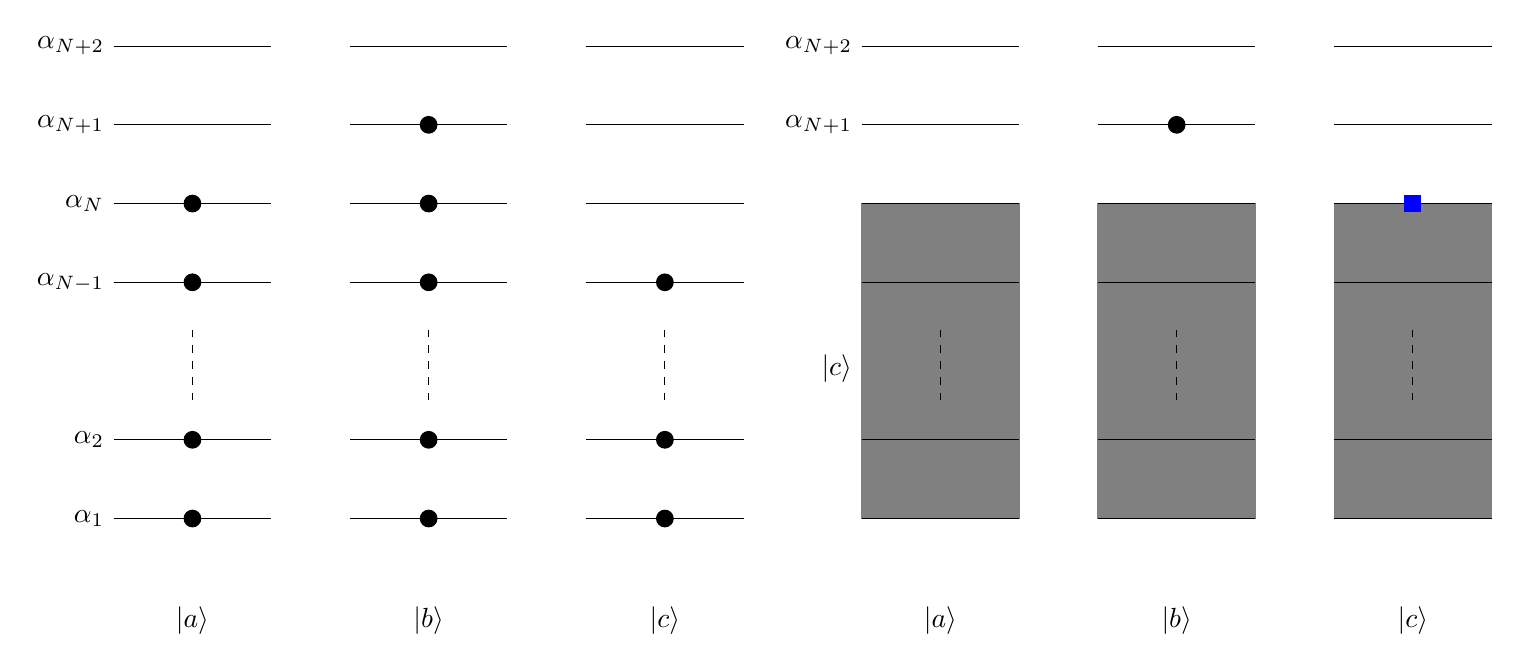
\begin{tikzpicture}
\draw (1,-1) node[anchor=north] {$\ket{a}$} -- (1,-1);
\draw (0,0) node[anchor=east] {$\alpha_1$} -- (2,0);
\draw (0,1) node[anchor=east] {$\alpha_2$} -- (2,1);
\draw (1,1.5) -- (1,1.6);
\draw (1,1.7) -- (1,1.8);
\draw (1,1.9) -- (1,2);
\draw (1,2.1) -- (1,2.2);
\draw (1,2.3) -- (1,2.4);
\draw (0,3) node[anchor=east] {$\alpha_{N-1}$} -- (2,3);
\draw (0,4) node[anchor=east] {$\alpha_N$}-- (2,4);
\draw (0,5) node[anchor=east] {$\alpha_{N+1}$}-- (2,5);
\draw (0,6) node[anchor=east] {$\alpha_{N+2}$} -- (2,6);
\filldraw [black] (1,0) circle (3pt);
\filldraw [black] (1,1) circle (3pt);
\filldraw [black] (1,3) circle (3pt);
\filldraw [black] (1,4) circle (3pt);

\draw (4,-1) node[anchor=north] {$\ket{b}$} -- (4,-1);
\draw (3,0) -- (5,0);
\draw (3,1) -- (5,1);
\draw (4,1.5) -- (4,1.6);
\draw (4,1.7) -- (4,1.8);
\draw (4,1.9) -- (4,2);
\draw (4,2.1) -- (4,2.2);
\draw (4,2.3) -- (4,2.4);
\draw (3,3) -- (5,3);
\draw (3,4) -- (5,4);
\draw (3,5) -- (5,5);
\draw (3,6) -- (5,6);
\filldraw [black] (4,0) circle (3pt);
\filldraw [black] (4,1) circle (3pt);
\filldraw [black] (4,3) circle (3pt);
\filldraw [black] (4,4) circle (3pt);
\filldraw [black] (4,5) circle (3pt);

\draw (7,-1) node[anchor=north] {$\ket{c}$} -- (7,-1);
\draw (6,0) -- (8,0);
\draw (6,1) -- (8,1);
\draw (7,1.5) -- (7,1.6);
\draw (7,1.7) -- (7,1.8);
\draw (7,1.9) -- (7,2);
\draw (7,2.1) -- (7,2.2);
\draw (7,2.3) -- (7,2.4);
\draw (6,3) -- (8,3);
\draw (6,4) -- (8,4);
\draw (6,5) -- (8,5);
\draw (6,6) -- (8,6);
\filldraw [black] (7,0) circle (3pt);
\filldraw [black] (7,1) circle (3pt);
\filldraw [black] (7,3) circle (3pt);

\draw (10.5,-1) node[anchor=north] {$\ket{a}$} -- (10.5,-1);
\filldraw [gray] (9.5,0) rectangle (11.5,4);
\draw (9.5,0) -- (11.5,0);
\draw (9.5,1) -- (11.5,1);
\draw (10.5,1.5) -- (10.5,1.6);
\draw (10.5,1.7) -- (10.5,1.8);
\draw (10.5,1.9) node[anchor=east] {$\ket{c}\hspace{1cm}$} -- (10.5,2);
\draw (10.5,2.1) -- (10.5,2.2);
\draw (10.5,2.3) -- (10.5,2.4);
\draw (9.5,3)  -- (11.5,3);
\draw (9.5,4)  -- (11.5,4);
\draw (9.5,5) node[anchor=east] {$\alpha_{{N+1}}$} -- (11.5,5);
\draw (9.5,6) node[anchor=east] {$\alpha_{N+2}$} -- (11.5,6);

\draw (13.5,-1) node[anchor=north] {$\ket{b}$} -- (13.5,-1);
\filldraw [gray] (12.5,0) rectangle (14.5,4);
\draw (12.5,0) -- (14.5,0);
\draw (12.5,1) -- (14.5,1);
\draw (13.5,1.5) -- (13.5,1.6);
\draw (13.5,1.7) -- (13.5,1.8);
\draw (13.5,1.9) -- (13.5,2);
\draw (13.5,2.1) -- (13.5,2.2);
\draw (13.5,2.3) -- (13.5,2.4);
\draw (12.5,3) -- (14.5,3);
\draw (12.5,4) -- (14.5,4);
\draw (12.5,5) -- (14.5,5);
\draw (12.5,6) -- (14.5,6);
\filldraw [black] (13.5,5) circle (3pt);

\draw (16.5,-1) node[anchor=north] {$\ket{c}$} -- (16.5,-1);
\filldraw [gray] (15.5,0) rectangle (17.5,4);
\draw (15.5,0) -- (17.5,0);
\draw (15.5,1) -- (17.5,1);
\draw (16.5,1.5) -- (16.5,1.6);
\draw (16.5,1.7) -- (16.5,1.8);
\draw (16.5,1.9) -- (16.5,2);
\draw (16.5,2.1) -- (16.5,2.2);
\draw (16.5,2.3) -- (16.5,2.4);
\draw (15.5,3) -- (17.5,3);
\draw (15.5,4) -- (17.5,4);
\draw (15.5,5) -- (17.5,5);
\draw (15.5,6) -- (17.5,6);
\filldraw [blue] (16.4, 3.9) rectangle (16.6,4.1) ;
\end{tikzpicture}}
\end{center}
\label{fig: Particle-hole figure}
\caption{Particle-Hole.}
\end{figure}

In the same way as we can construct a general slater determinant by letting the ordinary creation operators act on the vacuum state, we are now in a position to construct many-quasiparticle states by letting quasi-particle creation operators act on the reference state $\ket{r}$.
\begin{align}
\ket{ijkl..abcd..}_r \equiv \crequasi{i}\crequasi{j}\crequasi{k}\crequasi{l}..\crequasi{a}\crequasi{b}\crequasi{c}\crequasi{d}..\ket{r}.
\end{align}
To achieve the full potential of the particle-hole formalism, one would have to transform all operators to this representation. This is a tedious excersice which we will not include in this report. 

Wick's theorem in Eq. (\ref{def: Wick's theorem}) is valid for products of quasi-particle creation and annihilation operators, provided that the contractions are defined relative to the reference state. The only nonzero contributions are
\begin{align}
\contraction[0.5ex]{}{\anquasi{\alpha}}{}{\crequasi{\beta}} \anquasi{\alpha}\crequasi{\beta} = \for{r}{\anquasi{\alpha}\crequasi{\beta}}{r} = \delta_{\alpha\beta}.
\end{align}




















\clearemptydoublepage
\chapter{Second Quantization}
\label{chapsecondq}

When we are doing nuclear physics, we are actually studying many-particle systems. The difficult task in a many-body system 
is the interparticle potential. The nuclear case is not an exception.  
It turns out that a direct solution of the Schr\"odinger equation in configuration space is impractical, see for example Ref. \cite{fetter}.\\
\\
As mentioned in the last chapter a many-body problem may
seem impossible to solve. The problem complicates because of the interparticle potential. However the second quantization method has turned out to be a helpful and  practical tool when treating many-body physics.\\
\\
In second quantization one define the so-called creation operator,
$a^\dagger_\alpha$, which create a particle  and the annihilation operator
$a_\alpha$, which annihilate a particle. The subscript $\alpha$ indicates the
set of quantum number the particle have. A set of quantum numbers a particle
can have defines what is usually called a single-particle state.\\
\\
%In quantum mechanics the observables were quantized and described by operators, this is considered to
%be the first quantization. In second quantization  we are not only quantizing the observables, but also the particle states. 
%Each particle state is described by operators, we call them creation and annihilation operators, since they create
%and annihilate particles respectively.\\ 
The system studied in this thesis consists of nucleons which belong to the types
of particles called fermions. Fermions are particles with half integer spin. We
describe a system of fermions by an antisymmetric wave function, which
obey the Pauli principle. The Pauli principle states that two identical fermions
cannot have the same set of quantum numbers, ie.~they cannot be in the same
single particle state.\\
\\
As the case in this thesis, the
Hamiltonian takes the form \be H=\sum_{k=1}^Nt(x_k)+\frac{1}{2}\sum_{k \neq l
=1}^N v(x_k,x_l), \label{hamfirst} \ee  where $t$ is the kinetic energy and $v$
is the potential energy, the interactions between the particles. The letter
$x_k$ denotes the coordinates of particle $k$.  Since the potential energy term
represents the interaction between every pair of particles, counted once, we
need to multiply with the factor  $1/2$, see for example Ref.~\cite{fetter}, in
order to not double count.

\section{Creation and annihilation operators}

The interpretation of occupation of the antisymmetric many-body fermion
states allow us to introduce the two operators $a^\dagger_\alpha$ and 
$a_\alpha$, which create and annihilate a particle in the single particle 
state $\alpha$, which can be expressed as
\be
\begin{split}
& a^\dagger_\alpha \ket{0}=\ket{\alpha} ~ \mbox{and}~  a_\alpha \ket{\alpha}=\ket{0}
\end{split}
\ee 
respectively. The state vector $\ket{0}$ indicates the true vacuum.
The algebra of these operators depends on whether the system under 
consideration is a system of bosons or a system of fermions. If it consists of bosons the operators obey the commutation relations
\be
\begin{split}
& [a_k,a^\dagger_{k'}]=\delta_{k,k'}~\mbox{and}~ [a_k,a_{k'}]=[a^\dagger_k,a^\dagger_{k'}]=0,
\end{split}
\ee
while in the fermion case they obey the anti commutation relations
\be
\begin{split}
		& \{a_k,a^\dagger_{k'}\}=\delta_{k,k'}~ \mbox{and}~ \{a_k,a_{k'}\}=\{a^\dagger_k,a^\dagger_{k'}\}=0.
\end{split}
\ee
The Kronecker delta, \sd \delta_{k',k}\sd\,is equal to one if \sd k'=k\sd\, and zero else.\\
\\
With the above expressions for the commutators and anti-commutators
regarding the creation and annihilation operators the many-body Hamiltonian can 
be written as
\be
H=\sum_{ik} t_{ki}a^\dagger_ka_i + \frac{1}{2}\sum_{ijkl}v_{ijkl}a^\dagger_i
a^\dagger_ja_la_k.
\label{hamiltoniansec}
\ee
Many-body operators are denoted by capital letters in this text.\\
When the operators in the second quantization are non-relativistic and 
conserve the particle number, there should be an equal amount of creation
and destruction operators in the Hamiltonian. A second quantized 
many-body operator is written as a sum of one-particle operators, an operator 
that acts on one particle at a time as in Eq. \eqref{onesec}
\be
F=\sum_{\alpha,\beta}\bra{\alpha}f\ket{\beta}a^\dagger_\alpha a_\beta,
\label{onesec}
\ee 
and as a sum of two-particle operators in the form
\be
V=\frac{1}{2}\sum_{\alpha\beta\gamma\delta}\bra{\alpha\beta}v\ket{\gamma\delta}
a^\dagger_\alpha a^\dagger_\beta a_\delta a_\gamma.
\label{twosec}\\
\ee
\\
By using creation and annihilation operators we are able to write down a
many-body wave-function which we denote by capital Greek letters in contrast to 
single-particle states which are denoted by small Greek letters. A wave function
consisting of $N$ particles is written
as a product of $N$ creation operators,\\ $\ket{\Phi}
=a^\dagger_{1}(x_1)a^\dagger_2(x_2)a^\dagger_3(x_3)\cdots
a^\dagger_N(x_N)\ket{0}$. Here $x_1$ refers to the coordinates of particle 1,
the ket vector $\ket{0}$ still indicates the true vacuum and the subscript of
the creation operator refers to the single particle state the particle
occupies. The problem with this definition of the many-body wave function is
that it is not a symmetry eigenstate. By quantum mechanics every particle
should be able to occupy every single-particle state, $\varphi_i$, with a probability $p$. Since we now
are dealing only with fermions whose wave-function should be antisymmetric by
the interchange of two particles, we write the wave function as a determinant,
\be
\frac{1}{\sqrt{N!}}
\left|
\begin{array}{cccccc}
\varphi_i(x_1) & \varphi_j(x_1) & \varphi_k(x_1) & \varphi_l(x_1)& \cdots& \varphi_N(x_1) \\
\varphi_i(x_2) & \varphi_j(x_2) & \varphi_k(x_2) & \varphi_l(x_2)& \cdots& \varphi_N(x_2) \\
\varphi_i(x_3) & \varphi_j(x_3) & \varphi_k(x_3) & \varphi_l(x_3)& \cdots& \varphi_N(x_3)  \\
\varphi_i(x_4) & \varphi_j(x_4) & \varphi_k(x_4) & \varphi_l(x_4)& \cdots& \varphi_N(x_4) \\
\vdots & \vdots & \vdots & \vdots & \vdots& \vdots \\
\varphi_i(x_N) & \varphi_j(x_N) & \varphi_k(x_N) & \varphi_l(x_N)& \cdots& \varphi_N(x_N). \\
\end{array}
\right|
\label{eq:slaterdet}
\ee
In the many-body jargon this determinant is called a Slater determinant.\\
\\
%Interchanging two of the particles would be the same as interchanging two rows 
%in the Slater determinant, since this also changes the overall sign of the 
%determinant, obeying the anti-symmetry condition, this form of writing a many-body wave-function is 
%justified.
A more handy form to write the wave function, is as a permutation of every 
possible single-particle states $\varphi_i$. We rewrite the many-body wave-function as
\begin{equation*}
		\ket{\Phi}=\prod_{\substack{ij=1,\\i\neq j}}^NP(ij)a^\dagger_1(x_1)a^\dagger_2(x_2)a^\dagger_3(x_3)\cdots a^\dagger_N(x_N)\ket{0}.
\end{equation*}
The permutation operator $P(ij)$ is defined as when acting on
$a^\dagger_i(x_i)a^\dagger_j(x_j)$ gives $-a^\dagger_i(x_j)a^\dagger_j(x_i)$. 



\section{Wick's Theorem}
\label{wicksteorem}
A normal ordered second quantized operator is defined as an operator whose 
 annihilation operators stands to right of all creation operators. 
It is in some manner easier to calculate when the annihilation operators are
placed to the right.
Wick's theorem describes a fast method to put the annihilation operators to
the right of the creation operators, by using the anti commutation rules
for these operators. Before introducing Wick's theorem we present some
definitions like the normal product of operators and contractions of 
operators.\\ 
Given a product of creation and annihilation operators 
\beq
XYZ\cdots W,
\eeq
the normal product is defined as 
\beq
N(XYZ \cdots W),
\eeq
where all the destruction operators are moved to the right of the creation 
operators. As an example let us study the cases
\be
N(a^\dagger_\alpha a_\beta)=a^\dagger_\alpha a_\beta
\ee
and
\be
N(a_\alpha a^\dagger_\beta)=\pm a^\dagger_\beta a_\alpha,
\ee
where the minus sign applies for fermions only, and the
plus sign for bosons.\\ 
\\
One of the properties of a normal ordered product of operators is that the
vacuum expectation value of the product is zero, the destruction 
operator annihilates the vacuum state.\\
\\
A contraction of two operators $XY$ is defined as its  expectation value 
regarding the vacuum, $\ket{0}$,
\be
\wick{1}{<1a_\alpha >1a^\dagger_\beta}=\bra{0}a_\alpha a^\dagger_\beta\ket{0}=\bra{0}\delta_{\alpha\beta}-a^\dagger_\beta a_\alpha \ket{0}=\delta_{\alpha\beta}.
\label{contraction}
\ee  
By having defined the normal product and the contraction in Eq.~\eqref{contraction} we are now ready to 
state Wick's theorem which says that a product of randomly oriented 
creation and annihilation operators can be written as the normal product of
these operators plus the normal product of all possible contractions.
\be
XYZ\cdots W=N(XYZ\cdots W) + \sum^{\mbox{all possible}}_{\mbox{contractions}} N(XYZ \cdots W).
\label{wicks}
\ee
As a remark, in this theorem only fermions have been considered.
The proof of this theorem can be found in almost all books that treat 
quantum field theory or quantum theory of many-particles, see for example Ref.~\cite{heinonen}.



\section{The Particle-Hole Formalism}
\label{particlehole}
In a theory of many-particles, it is often more convenient to use another
state as reference state rather than the vacuum state. This reference state
should be a stable state. The normal ordering will then be altered from the one 
given above for the true vacuum state, it is written 
$\ket{\Phi_0}=a^\dagger_ia^\dagger_j \cdots\ket{0}$. A new definition of the
creation and destruction operators is needed. The operators will now create and 
annihilate holes and particles. The definition of a hole is a one-particle
state that is occupied in the reference state $\ket{\Phi_0}$, while a 
particle state is a one-particle state that is not occupied in $\ket{\Phi_0}.$
This new nomenclature is easily understood when considering that a "hole" is
created when an originally occupied state is acted upon by an annihilation 
operator such as $a_i.$ A "particle" is created when an unoccupied state is
acted upon by a creation operator. These operators that destroy and create 
holes and particles are called quasiparticle 
operators. A q-annihilation operator annihilates holes and particles, 
while a q-creation operator creates holes and particles.\\ 
\\
A normal ordered product of quasiparticle operators would then be defined as
a product where all the quasiparticle destruction operators stand to the right
of all the quasiparticle creation operators. This definition of the normal 
ordered product changes the analysis of Wick's theorem. The only
contractions that contribute are the ones where a destruction operator 
stands to the left of a creation  operator, there are two ways this can 
happen
\be
\begin{split}
& \wick{1}{<1a_i^\dagger>1a_j}=a^\dagger_i a_j-N(a^\dagger_ia_j)=a^\dagger_i
a_j+a_ja^\dagger_i=\delta_{ij}\\
& \wick{1}{<1a_i>1a^\dagger_j}=a_ia^\dagger_j-N(a_ia^\dagger_j)=a_ia^\dagger_j+a^\dagger_ja_i=\delta_{ij}.
\label{normalhole}
\end{split}
\ee
That is if $i$ defines a hole state in Eqs. \eqref{normalhole}.
As an example, consider normal ordering of a two particle Hamiltonian, as 
in the following equation
\be
\hat H = \sum_{pq}\bra{p}h\ket{q}a^\dagger_p a_q + \frac{1}{4}\sum_{pqrs}
\bra{pq}V\ket{rs}a^\dagger_p a^\dagger_qa_sa_r
\label{twoham}
\ee
The one-particle part  is written as 
\be
\sum_{pq}\bra{p}h\ket{q}N(a^\dagger_p a_q)+\sum_{i\in hole}\bra{i}h\ket{i}.
\label{eq:normen}
\ee
The two-particle part is rewritten as 
\be
\begin{split}
& \frac{1}{4}\sum_{pqrs} \bra{pq}V\ket{rs}a^\dagger_p a^\dagger_pa_sa_r=
 \frac{1}{4}\sum_{pqrs} \bra{pq}V\ket{rs}N(a^\dagger_p a^\dagger_q a_s a_r)
+\\ &\sum_{ipq}\bra{pi}V\ket{q i}N(a^\dagger_pa_r)+\frac{1}{2}\sum_{ij}\bra{ij}V\ket{ij}
\label{normH}.
\end{split}
\ee
For the entire calculation see Ref. \cite{sjefer}.
After the equal sign in Eq. \eqref{normH} the letters $p,q,r,$ and $s$ indicate 
both hole and particle states, while the letters $i$ and $j$   indicate hole states.
By combining the terms in equations \eqref{eq:normen} and \eqref{normH} we write
the entire Hamiltonian as
\be
\begin{split}
&H=\sum_{pq}\bra{p}h\ket{q}N(a^\dagger_p a_q)+\sum_i\bra{i}h\ket{i}+
\frac{1}{2}\sum_{ij}\bra{ij}V\ket{ij}+\\
& \frac{1}{4}\sum_{pqrs} \bra{pq}V\ket{rs}N(a^\dagger_p a^\dagger_q a_s a_r)
+\sum_{ipq}\bra{pi}V\ket{qi}N(a^\dagger_p a_q),
\label{normalham}
\end{split}
\ee
where $p,q,r,$ and $s$ still run over all states, $i$ and $j$ over hole states only.

\clearemptydoublepage
\chapter{Perturbation Theory}
\label{projection}

This chapter will treat perturbation theory, as the title indicates, and it is mainly based on the work in Ref. \cite{realeff}.\\
\\
The many-body Schr\" odinger equation is rather difficult to solve. 
Even a two body problem is a rather complicated system to solve, that is why
we have to come up with approximated methods such as perturbation theory.
The starting point is usually to separate the Hamiltonian 
in an unperturbed part and a perturbed part. The perturbed part is
the one which considers the interactions between the particles. We write the Schr\"odinger equation as
\be
H\Psi=(H_0 +V_I)\Psi=E\Psi,
\ee
where $H_0$ is the unperturbed Hamiltonian with a known solution. The unperturbed Hamiltonian is a sum of one-particle operators, $h_0$, 
which in most of the problems governing nuclear physics is a harmonic 
oscillator Hamiltonian. The unperturbed part is written as $H_0=T + U$,
where $T$ denotes the kinetic energy of the system and $U$ is the single 
particle potential. We write  the 
perturbed part as $V_I = V-U.$

Obviously the difference $V-U$ should be small enough so that
 treating $V_I$ as a perturbation is valid. The exact result is independent of the one particle potential $U$, but 
in an approximated calculation it is possible that the results depend on the one-particle potential that is included in
the calculations. The eigenfunctions, $\Phi_i$ of the unperturbed Hamiltonian 
are taken as a basis for the expansion of the eigenfunction $\Psi$,
\be
\ket{\Psi}=\sum_{i=1}\alpha_i\ket{\Phi_i}.
\ee
To simplify the calculations it is common practice to divide the space in a model space and an excluded 
space. By doing this we define 
two projection operators, that we will meet again later. These projection operators are denoted by a $P$ and a $Q.$ The $P$ operator projects
the complete wavefunction onto the model space 
\be
P\ket{\Psi}=\ket{\Psi_M},
\ee
while $Q$ is the complimentary projection operator and connects the complete wavefunction with the excluded state $\ket{\Psi_Q}.$ They are written as
\be
\begin{split}
P=\sum_{i=1}^d \ket{\Phi_i}\bra{\Phi_i}~\mbox{and}~ Q=\sum_{i=d+1}^N \ket{\Phi_i}\bra{\Phi_i}
\end{split}
\ee
The projection operators satisfy the properties
\be
\begin{split}
P^2=P,~Q^2=Q,~PQ=QP=0~\mbox{and}~P+Q=1.
\end{split}
\label{projectionopprop}
\ee
Since $\mathcal E_k$ are the eigenvalues of the unperturbed Hamiltonian $H_0$, we obtain that 
\be
(E-\mathcal E_j)\alpha_j=\bra{\Phi_j}V\ket{\Psi}.
\label{differense}
\ee
By using this relation we write the entire wavefunction $\ket{\Psi}$  as
\beq
\ket{\Psi}= \sum_{i=1}^d \alpha_i\ket{\Phi_i} + \sum_{i=d+1}^N\frac{\ket{\Phi_i}\bra{\Phi_i}V\ket{\Psi}}{E-\mathcal E_i}=\sum_{i=1}^d\alpha_i\ket{\Phi_i} + \frac{QV}{E-H_0}\ket{\Psi}= P\ket{\Psi} + \frac{QV}{E-H_0}\ket{\Psi}.
\eeq
If we now define a wave operator which projects the model space onto the complete wavefunction $\Omega\ket{\Psi_M}=\ket{\Psi}$ we find it to be
\be
\Omega(E)=1 + \frac{Q}{E-H_0}V\Omega(E).
\ee
By using the wave operator in Eq \eqref{differense} we get 
\be
(E-\mathcal E_j)\alpha_j=\bra{\Phi_j}V\Omega\ket{\Psi_M}=\sum_{k=1}^d\bra{\Phi_j}V\Omega\ket{\Phi_k}\alpha_k
\ee
which is equivalent to 
\be
[H_0 + V\Omega(E) -E]\Psi_M=0.
\ee
We will define an effective interaction 
\be
\mathcal V(E)=V\Omega(E)
\ee
to get an integral equation, 
\be
\mathcal V(E)=V + V\frac{Q}{E-H_0}\mathcal V(\Omega),
\label{effektivvv}
\ee
for the effective interaction, which is dependent on the energy $E$. 
Equation \eqref{effektivvv} can be solved by iteration, where we by using $V$ as
a first guess find that
\be
\begin{split}
&\mathcal V(E)=V + VQ\frac{1}{E-H_0}QV +VQ\frac{1}{E-H_0}QVQ\frac{1}{E-H_0}QV
+\\
& VQ\frac{1}{E-H_0}QVQ\frac{1}{E-H_0}QVQ\frac{1}{E-H_0}QV + \cdots~.
\end{split}
\ee
This can be solved analytically by observing that the expression above resembles
a geometric sum, one rewrite it as 
\be
\begin{split}
\mathcal V=V + VQ\frac{1}{E-H_0-QVQ}QV=PVP + PVQ\frac{1}{E-QHQ}QVP.
\end{split}
\ee


\section{Time dependent perturbation theory}


When doing time dependent perturbation theory we have to define a time 
evolution propagator $U(t,t')$. The time evolution operator evolves a state 
$\Psi(t')$ at time $t'$ to a state $\Psi(t)$ at 
time $t$ 
\be
\Psi(t)=U(t,t')\Psi(t').
\ee
The wavefunctions satisfy the time dependent Schr\" odinger equation, 
\be
\begin{split}
&i \frac{\partial}{\partial t}\Psi(t)=H\Psi(t)\\
&i \frac{\partial}{\partial t}\Psi(t)=i \frac{\partial}{\partial t}\left[U(t,t')\Psi(t')\right],
\end{split}
\ee
which yields that the time evolution operator satisfies the time dependent Schr\"odinger equation.
By solving the equation we find the time evolution operator to be
\be
U(t,t')=e^{-iH(t-t')}.
\ee
This form of the time evolution operator gives right away the properties one 
would expect of an operator of this kind. These properties can be summarized as

\be
U(t,t)=1,~U(t',t)U(t,t')=1
\ee
and
\be
U(t,t')U(t,t')^\dagger= ~U(t,t')^\dagger U(t,t')=1,
\ee
From these definitions it follows that the complex conjugate of the time evolution
operator is also its inverse and that interchanging $t$ and $t'$ is the same as
taking the complex conjugate, see below, 
\be
U(t',t)=U(t,t')^\dagger=U(t,t')^{-1},~
U(t_1,t_2)U(t_2,t_3)=U(t_1,t_3).
\ee\\
\\
By use of Gell-Mann's theorem Ref. \cite{thouless}, exact eigenstates can be constructed
through the action of the time-development operator.  In the present approach
the time $t$ will be rotated by a small angle $\epsilon$, thus $t$ is a complex quantity.\\
We write the eigenstate as
\be
\frac{\ket{\Psi_i}}{\braket{\Phi}{\Psi_i}}=\substack{lim\\ \epsilon \rightarrow 0}\, \substack{lim\\t'\rightarrow\\-\infty(1-i\epsilon)}
\frac{U(t,t')\ket{\Phi}}{\bra{\Phi}U(t,t')\ket{\Phi}},
\label{eigenstatefortime}
\ee
where $\ket{\Psi_i}$ is the lowest state of $H$ with $\braket{\Phi}{\Psi_i}\neq
0.$ This relationship is very useful in calculating the ground state energy
shift $\Delta E_0.$\\
\\
If our unperturbed Hamiltonian gives the energy $E_0$ while acting on the
unperturbed state $\ket{\Phi}$, and our total energy is $E,$ the ground state
energy shift is given by
\be
\begin{split}
&\Delta E_0=E-E_0=\frac{\bra{\Phi}V\ket{\Psi}}{\braket{\Phi}{\Psi}}\\
&=\substack{lim\\ \epsilon \rightarrow 0^+}\substack{lim \\t'\rightarrow \\
 -\infty(1-i\epsilon)}\frac{\bra{\Phi}VU(0,t')\ket{\Phi}}{\bra{\Phi}U(0,t')\ket{\Phi}}.
\label{energyshift1}
\end{split}
\ee
To evaluate this as a perturbation, we expand the time evolution
operator $U(t,t')$. This is most conveniently done in the so-called interaction
picture, to be explained below. See also Refs.~\cite{shankar94,sakurai} for 
more details.
The interaction picture can be understood as an intermediate between the Schr\" odinger picture and the Heisenberg picture. In the Schr\" odinger picture the 
operators are time independent while the state evolves with time. It is all
contrary in the Heisenberg picture where the operators now are time dependent
and the state is time independent.
In the interaction picture both the state vectors and the operators are time
dependent, however their time dependencies are somehow different.\\
\\
A state vector in the interaction picture is defined as
\be
\ket{\psi_I(t)}=e^{iH_{0,S}t}\ket{\psi_s(t)},
\ee
where the letter $S$ stands for the Schr\" odinger picture. Operators in the interaction picture are defined as
\be
A_{I}(t) = e^{i H_{0,S} t} A_{S}(t) e^{-i H_{0,S} t },
\ee
where $H_0$ is the unperturbed Hamiltonian. The time evolution of the operators is given by 
\be
i\frac{d}{dt}A_I(t)=\left[A_I(t),H_0\right].\; 
\label{timevop}
\ee
By using the definition of one-particle and two-particle operators from chapter
\ref{chapsecondq}, our Hamiltonian can be written as in Eq.
 \eqref{hamiltoniansec}, we write it again here as
\beq
H=\sum_{k} \epsilon_{k}a^\dagger_ka_k + \frac{1}{2}\sum_{ijkl}V_{ijkl}a^\dagger_i
a^\dagger_ja_la_k.
\eeq
From Eq.~\eqref{timevop} we see that it suffices to find the time
evolution of the creation and annihilation operators $a^\dagger$ and $a$ to find the time evolution of the Hamiltonian. The commutator between the creation operator and the unperturbed Hamiltonian is 
\be
\left[a^\dagger_k,H_0\right]=-\epsilon a^\dagger_k(t)
\ee
thus we obtain the time dependence of the creation and destruction operators as
\beq
\begin{split}
& a^\dagger(t)_k=a^\dagger_ke^{i\epsilon_kt}
\end{split}
\eeq
and
\beq
\begin{split}
& a(t)_k=a_ke^{-i\epsilon_kt}
\end{split}
\eeq
respectively.\\
\\
We will now transform the Schr\" odinger equation to the interaction picture
\be
\begin{split}
&\psi_I(t)=e^{iH_0t}\psi(t)\\
&=e^{iH_0t}U(t,t')e^{-iH_0t'}e^{iH_0t'}\psi(t')\\
&=U_I(t,t')\psi_I(t')
\end{split}
\label{itertimeop}
\ee
By differentiating Eq. \eqref{itertimeop} with respect to time $t$ we find that
\be
\frac{\partial}{\partial t}U(t,t')=VU(t,t').
\ee\\
When we have found how the time evolution operator behaves with time, we may also find the 
perturbative expansion of the time evolution operator. The solution to the differential equation is 
\be
U(t,t')=1  -i\int_{t'}^tdt_1V(t_1)U(t_1,t')
\label{ekspavtidev}
\ee
Equation \eqref{ekspavtidev} can be solved by iteration using
\be
U(t,t')=1+\sum_{n=1}^\infty\left(-i\right)^n\int_{t'}^tdt_1
\int_{t'}^{t_1}dt_2\cdots \int_{t'}^{t_{n-1}}dt_nV(t_1)V(t_2)\cdots V(t_n).
\ee
%of the time evolution operator.
%The above form of the time evolution operator can be inserted into Eq. 
%\eqref{eigenstatefortime}, which gives us the perturbative expansion for
%calculating the interactions.


\section{Feynman-Goldstone diagrams}

To evaluate Eq. \eqref{eigenstatefortime} we had to define a new operator, called the time ordering operator. The effect of the time ordering operator on a 
product of operators is to order the them so the operators with a larger
time argument are placed to the left to those of smaller time arguments. Since we in nuclear physics are dealing with fermions which obey the Pauli exclusion
principle there will be a sign dependency on the number of permutations needed 
in making the arrangement. As an example 
\be
\begin{split}
T\left[A_1(t_1)A_2(t_2)\cdots A_n(t_n) \right]\\
=(-1)^pA_\alpha(t_\alpha)A_\beta(t_\beta) \cdots A_\gamma(t_\gamma)
\end{split}
\ee
If we use time ordering together with the particle hole formalism from section \ref{particlehole}, we will find a new definition of the contraction.
A contraction of two operators will now be defined as
\be
\wick{1}{<1A>1B}=T[AB]-N[AB], 
\ee
where $N[AB]$ is the normal ordering operator. 
As an example we will derive a contraction 
of two hole operators and a contraction of two particle operators. 
We will first start with a contraction of two hole operators where both 
particles have momenta below $k_F,$ and with $t < t'.$
\be
\begin{split}
&\wick{1}{<1a_h(t)>1a_{h'}^\dagger (t')}=T\left[a_h(t)a_{h'}^\dagger (t')\right]
-N\left[a_h(t)a_{h'}^\dagger (t')\right]\\
&=-a_{h'}^\dagger (t')a_h(t)-a_h(t)a_{h'}^\dagger(t')\\
&=-\left(a^\dagger_{h'}(t')a_h(t)+a_h(t)a_{h'}^\dagger(t')\right)e^{-i(\epsilon_ht-\epsilon_{h'}t')}\\
& = -\delta_{h,h'}e^{-i(\epsilon_ht-\epsilon_{h'}t')}.
\end{split}
\label{kontrakt1}
\ee
Similarly for particles with momenta above $k_F$ and $t<t'$
\be
\wick{1}{<*a_p(t)>*a_{p'}(t')}=\delta_{p,p'}e^{-i\epsilon_p(t-t')}
\label{kontrakt2}
\ee
We have 
\be
\wick{1}{<*a_\alpha(t)>*a_\beta^\dagger(t')}=-\wick{1}{<*a_\beta^\dagger(t')>*a_\alpha(t)}
\ee
\begin{figure}[htp]
\centering
\includegraphics[scale=0.5]{hullpartlinje}
\caption{Diagrammatic representation of the contractions in Eqs. 
\eqref{kontrakt1} and \eqref{kontrakt2} The time is going upward.}
\label{hullpartlinje}
\end{figure}\\
\\
In Fig (\ref{hullpartlinje}) the two contractions in Eqs \eqref{kontrakt1} 
and \eqref{kontrakt2} are represented diagrammatically, the annihilation 
operator $a_\alpha$ destroys the particle line $a^\dagger_\beta$ creates. The
time is upward.\\
\\
With the above definitions of time ordering and contractions we are ready to go back to the time evolution operator, which is already in a time ordered 
form
\be
U(t,t')=\sum_{n=0}^\infty\left(-i\right)^n\int_{t'}^tdt_1
\int_{t'}^{t_1}dt_2\cdots \int_{t'}^{t_{n-1}}dt_nT\left[V(t_1)V(t_2)\cdots V(t_n)\right].
\label{tidevolusjon1}
\ee
From  Eq. \eqref{tidevolusjon1} we see that there are $n!$ ways to order the multidimensional
integral with respect to the times $t_1,t_2 \cdots t_n$, it is again possible to
rewrite the time evolution operator to the form
\be
U(t,t')=\sum_{n=0}^\infty\frac{1}{n!}\left(-i\right)^n\int_{t'}^tdt_1
\int_{t'}^{t}dt_2\cdots \int_{t'}^{t}dt_nT\left[V(t_1)V(t_2)\cdots V(t_n)\right]
\label{tidevolusjon2}
\ee\\
If we recall that it is the energy shift we want to calculate, we can use the 
above equation to write the numerator and the denominator in Eq. 
\eqref{energyshift1} as
\be
%\begin{split}
%&\Delta E_0=\substack{lim\\ \epsilon \rightarrow 0^+}\substack{lim \\t'\rightarrow \\
% -\infty(1-i\epsilon)}\frac{\bra{\phi}VU(0,t')\ket{\phi}}{\bra{\phi}U(0,t')\ket{\phi}}\\
\sum_{n=0}^\infty\frac{1}{n!}\left(-i\right)^n\int_{t'}^tdt_1
\int_{t'}^{t}dt_2\cdots \int_{t'}^{t}dt_n\bra{\phi}T\left[V(t)V(t_1)V(t_2)\cdots V(t_n)\right]\ket{\phi}
\ee
and
\be
 \sum_{n=0}^\infty\frac{1}{n!}\left(-i\right)^n\int_{t'}^tdt_1
\int_{t'}^{t}dt_2\cdots \int_{t'}^{t}dt_n\bra{\phi}T\left[V(t_1)V(t_2)\cdots V(t_n)\right]\ket{\phi}
%\end{split}
%\label{energyshift2}
\ee
respectively.
%Where $V(t)$ in the numerator in  Eq. \eqref{energyshift2} is put into to 
%the time ordering operator. 
To evaluate the integrals in the numerator and the
denominator we have to use Wick's theorem, Wick's theorem with time ordering
will be slightly modified from the first version in section \ref{wicksteorem}. Wicks theorem states now that\\ 
\be
\begin{split}
&T\left[A(t_1)B(t_2)C(t_3) \cdots Z(t_n)\right]=N\left[A(t_1)B(t_2)C(T_3) \cdots Z(t_n)\right]\\
&+ \sum_{1\, contraction}N\left[A(t_1)B(t_2)C(T_3) \cdots Z(t_n)\right]+\sum_{2\, contractions}N\left[A(t_1)B(t_2)C(T_3) \cdots Z(t_n)\right]\\
&+ \cdots + \sum_{\substack{contractions\, with\\ all \, operators}}N\left[A(t_1)B(t_2)C(T_3) \cdots Z(t_n)\right].\\
\end{split}
\label{wicktheofortime}
\ee
Since our unperturbed state is the groundstate, our reference vacuum state, only the last term in Eq. \eqref{wicktheofortime} survives. % We are 
%left with the term where all operators are participating in the contractions. 
Further all unlinked diagrams in the numerator, ie.~all contractions which 
does not include the interaction $V(t)$ are canceled by the diagrams
in the denominator.\\
\\
Let us now evaluate the first-order contribution to the energy shift in Eq. \eqref{energyshift1}. The only contributing term is $V(t)$ which on 
a second quantized form is written as\\ $v_{\alpha\beta\gamma\delta}a^\dagger_\alpha(t) a^\dagger_\beta(t) a_\delta(t) a_\gamma(t).$
From Wick's theorem we will then have two terms contributing to the energy 
shift.
\be
\begin{split}
\wick{21}{<*a^\dagger_\alpha(t) <2a^\dagger_\beta(t) >2 a_\delta(t) >*a_\gamma(t)} +
\wick{21}{<*a^\dagger_\alpha(t) <2a^\dagger_\beta(t) >* a_\delta(t) >2a_\gamma(t)} 
\end{split}
\label{forsteordenbidrag}
\ee
The terms in Eq. \eqref{forsteordenbidrag} can be depicted diagrammatically 
as seen in Fig~\ref{forsteordendiagram}.
\begin{figure}[htp]
\centering
%\includegraphics[height=0.8\textheighti]{forsteordendiagram}
\includegraphics[scale=0.5]{forsteordendiagram}  %[width=1.0\textwidth]{forsteordendiagram}
\caption{Diagrammatic representation of the first order diagram, the diagram to the left depicts the first term in Eq. \eqref{forsteordenbidrag}, the 
diagram to the right depicts the second term in Eq. \eqref{forsteordenbidrag}.}
\label{forsteordendiagram}
\end{figure}
The single particle states $\alpha, \, \beta, \, \gamma$ and $\delta$ must all be holes, since they are all equal time operators.
The energy shift can now be written as 
\be
\Delta E_0=	 \frac{1}{2}\sum_{\alpha\beta < k_f} \frac{1}{2}(v_{\alpha\beta\alpha\beta}-v_{\alpha\beta\beta\alpha}),
\ee
the minus sign comes in, by the "rule" that for every contraction that crosses
another one, contributes with a factor $(-1).$
\begin{figure}[htp]
\centering
%\includegraphics[height=0.8\textheighti]{forsteordendiagram}
\includegraphics[scale=0.5]{perturbdiag}  %[width=1.0\textwidth]{forsteordendiagram}
\caption{Diagrammatic representation of second to third order contribution to the energy.}
\label{perturbdiagdiagram}
\end{figure}\\
\\
Fig~\ref{perturbdiagdiagram} depicts second- and third-order contributions to
the energy, with the rules for computing the diagrams 
the second order contribution is
\be
\Delta E^{(2)}= \frac{\bra{ij}V\ket{ab}\bra{ab}V\ket{ij}}{\epsilon_{ij}-\epsilon_{ab}},
\ee
where $\epsilon_{pq}=\epsilon_p + \epsilon_q$, denotes the single particle 
energies and the indexes $i$ and $j$ runs over states occupied in the reference vacuum and $a$ and $b$ runs over single-particle states not occupied in the reference vacuum.\\
\\
With the clever invention of diagrams that depict the contractions, we are
able to describe every term in the expansion of the time evolution operator as
diagrams. These diagrams are usually called Feynman diagrams or
Feynman-Goldstone diagrams, to honor the inventors.  When presenting all the
terms as diagrams we need some rules to keep track of them. The idea is that we
find a term in the expansion by studying the corresponding diagram. A nice derivation of the diagram
rules can be found in Ref. \cite{kuo1981}.  The rules are summarized in appendix
\ref{diagramregler}. 




 % vlowk.tex
\clearemptydoublepage
\chapter{Nuclear matter} 

Nuclear matter is an idealized theoretical system of nucleons, it is a nucleus
composed of infinitely many nucleons. This chapter will review some of the
properties of  nuclei. It is unfortunately impossible to cover all the physics
concerning nuclear physics, and the author humbly have to admit that much of it 
is still unclear. We will first go through the nuclear forces and nuclear
structure before we finish the chapter with the shell model. 



\section{Nuclear structure} 
\label{sec:semiemp}
%Different nuclei are
%composed of different amounts of nucleons, there exists some 
%similarities between different nuclei. By study the binding energies, the difference of it rest energy from the nucleons in terms of the nucleus' mass,
The binding energy, $B(N,Z)$, is given by
\be
B(N,Z)=\big( Nm_n+Zm_p -M(N,Z) \big),
\ee
where $N$ is the neutron number and $Z$ is the proton number. The binding energy
is almost proportional to the number of particles (both protons and neutrons), 
$A$, composing the nucleus, see Ref.\cite{siemenselementsnuclei}.\\
%\be
%B(A) \approx bA.
%\ee
It is also found by experiments that the radius, $R$, of a nucleus increases with the number of particles, $R=r_0A^{1/3}.$ The value of $r_0$ is estimated by experiments to be approximately  $1.2$ fm, see for example \cite{kraneintro}. When the nucleus is considered to be spherical, the volume, 
$\Omega=4 \pi R^3/3,$ is linearly dependent on the number of particles, as a consequence the particle density in a nucleus is independent of the number of constituents. By dividing the volume by the number of constituents in a nucleus results in a particle density on the form
\be
\frac{A}{\Omega}=\frac{3}{4\pi r_0^3}\approx 1.95 \times 10^{38} \,\mbox{particles/cm}^3\\
\ee
\\
Since the volume of a nucleus depends linearly on the number of particles (as a droplet does), we can 
model the nucleus with a liquid drop. With the liquid drop model we are able to find a formula
for the mass of a nucleus.  Since this formula is obtained with both empirical
data and theoretical assumptions this formula is called the semi-empirical mass
formula. The binding energy has (by using scattering data on nucleon-nucleon interaction) been parametrized as
\be
    B = a_{v} A - a_{S} A^{2/3} - a_{C} \frac{Z(Z-1)}{A^{1/3}} - a_{A} \frac{(A - 2Z)^{2}}{A} + \delta(A,Z).
\label{eq:semibinding}
\ee
 The first term is called the volume term, this term satisfy the almost linearly dependence on the nucleon number $A$.
 This linearly dependence of $A$ indicates that each nucleon attracts only it closest neighbors and not all the other
nucleons. Since we from experiments, such as electron scattering, have concluded
that the nucleus density is constant, every nucleon has the same amount of
closest neighbors. The exception are those nucleons that lie on the surface of
the nucleus, thus we have to subtract this term, since the term $a_vA$ is an
overestimate. The surface nucleons contribute with a negative term
$-a_sA^{2/3}.$ The repulsive coulomb term of the protons should also be taken
into consideration, assuming a uniformly charged sphere, we obtain that the
contribution is 
\beq
-a_{C} \frac{Z(Z-1)}{A^{1/3}}. 
\eeq
There are two more terms left,
which are mainly extracted from experiments.
The first one is called the asymmetry term, it accounts for the effect that
the most stable nuclei are symmetric, we include the term 
\beq
- a_{A} \frac{(A -2Z)^{2}}{A}.
\eeq
The last term is the pairing term, which accounts for the fact
that the most stable configuration is when the number of nucleons of the same kind  with spin up
is equal to the number of nucleons with spin down, which is a property because
of the Pauli principle.  The pairing term does not contribute if we have an odd
number of nucleons, but affect the mass or binding energy differently in the
two cases of even-even nuclei and odd-odd nuclei, we give it the symbol
$\delta(A,Z)$, its contribution to the formula is
\beq
    \delta(A,Z) = \begin{cases} +\delta_{0} & Z,N \mbox{ even } (A \mbox{ even}) \\ 0 & A \mbox{ odd} \\ -\delta_{0} & Z,N \mbox{ odd } (A \mbox{ even})\end{cases} \\
\eeq
To find the mass of a given nucleus we subtract the binding energy from the sum of the nucleon masses as done here;
\be
 m = Z m_{p} + N m_{n} - \frac{B}{c^{2}}.
\ee



\section{A review of nuclear forces}

The mere existence of the deuteron is an evidence of the nuclear force, or the
strong force, and that the force between protons and neutrons have to be
attractive at least in the $J^\pi = 1^+$ state, or the $^3S_1$ partial wave state, which carries the quantum numbers  of the deuteron.\\
\\
Interference between Coulomb and
nuclear scattering for the proton-proton partial wave $^1S_0$
shows that the nucleon-nucleon force is attractive at least for the $^1S_0$
partial wave, and that it has to be greater than the coulomb force at small distances.
If not the protons would have been repelled by the repulsive
electromagnetic forces the protons mediates with each other. However
for interparticle distances of atomic scale, the nucleon-nucleon interaction (of the strong force) is negligible.
The cross section for neutron-proton scattering is isotropic for
energies up to 10 MeV in the center of mass frame, it is then concluded that
the scattering occurs in the relative $S$ states.\\
\\
The nuclear force which is the same as the strong force, the one of quarks
and gluons.  The same force that holds the nucleus together is the same that
keeps together the quarks that combine to make hadrons. Hadrons are particles
that feel the strong force and are composite of quarks. The nucleons consist of
the up, $u$ and down, $d$ quarks.  There are three generations of quarks, six quarks
in total. Beside the already mentioned $u$ and $d$ quarks, we have the charm quark, $c$, strange quark $s$, the top quark $t$ and the bottom quark $b$. They were not all discovered at the same time, the most heavy,
the top quark was not discovered until 1995 by the CDF and D0 experiments at Fermilab, \cite{PhysRevLett.74.2422,PhysRevLett.74.2626}. We state the 
three generations of quarks as
\be
\begin{pmatrix}
u \\
d
\end{pmatrix},
\begin{pmatrix}
c\\
s
\end{pmatrix}
\mbox{and}
\begin{pmatrix}
t\\
b
\end{pmatrix}.
\ee
All quarks have both electric charge
and color charge. The electric charges differ by $e$ in each generation, where
the upper ones have $2/3e$ and the lower have charges $-1/3e,$ where $e$ is the
electron charge.  There are three types of color charges red blue and
green. The quarks are spin half particles which have to obey the Pauli principle.\\
\\
The nucleons, the proton and neutron consist of three quarks. The proton
consists of two $u$ quarks and one $d$ quark which combine to the electric
charge of one $e$. The neutron consists of two $d$ quarks and one $u$ quark
which make the neutron electrically neutral.\\
%Since the quarks are fermions and
%there exists hadrons where two of the same type of quarks are found to be in the
%same state, radial and spin state it was deduced that there must be an 
%extra quantum number identifying the quarks. This quantum number was named 
%color.\\ 
%!!!I have to check this
%In the last section I argued that the density is constant in the nuclei.  It
%does not matter how many nucleons you put into the system, the density remains
%the   same. This indicates that there is a repulsive core at very short
%distances, experimentally it is found to be at $\approx 0.5$ fm.\\
\\
Much of what is known about nucleons is by combinations of experiment and 
theoretical predictions. Much is known by nucleon-nucleon scattering. 
By calculating the differential cross section for nucleon-nucleon 
scattering it is understood that the nuclear potential is not just dependent on 
the coordinates but also on the spin of the particles.
The definition of the differential cross section $d\sigma/d\Omega,$ is the probability per unit solid angle that an incident particle is scattered into the
solid angle $d\Omega.$ The standard unit for measuring a cross section is the barn, b, and it is equal to $10^{-28}$m$^2$. The probability $d\sigma$ that an incident particle is 
scattered into $d\Omega$ is the ratio of the scattered current through $d\Omega$
to the incident current, see Ref. \cite{kraneintro}
\be
d\sigma = \frac{(j_{scattered})r^2d\Omega}{j_{incident}}
\label{Eq:crossec}
\ee
If we use that the current of the particles is
%%SHOW IT
\be
\bold{j}= \frac{1}{2mi}(\psi^*\nabla \psi- (\nabla\psi^*)\psi),
\ee
which is found by multiplying the Schr\"odinger equation with $\psi^*$,
\begin{equation*}
		\begin{split}
		i\psi^*\frac{\partial\psi}{\partial t}+\frac{1}{2m}
		\psi^*\nabla^2 \psi= i\frac{\partial}{\partial t}(\psi^*\psi)
		-i\frac{\partial \psi^*}{\partial t}\psi+\frac{1}{2m}\psi^*\psi\\
		=i\frac{\partial}{\partial t}(\psi^*\psi)+\frac{1}{2m}\nabla\left(\psi^*\nabla\psi-(\nabla\psi^*)\psi\right)=0\Rightarrow \frac{\partial \rho}{\partial t}+\bold{\nabla}\cdot \bold{j}=0,
\end{split}
\end{equation*}
where $\rho=\psi^*\psi$ is interpreted as the probability density.\\ 
It is just a matter of finding the wave function to calculate the cross section. We let the incoming wave have the form
\be
\psi_{incident}=\frac{A}{2ik}\left[\frac{e^{ikr}}{r}-\frac{e^{-ikr}}{r} \right].
\label{incident}
\ee
This form keeps the incident wave finite as $r \rightarrow 0.$ By assuming that the scattering cannot create or destroy particles, but only
change the phase of the outgoing wave, the total wavefunction can be written as
\be
\psi(r)=\frac{A}{2i}e^{-i\delta}\left[ \frac{e^{i(kr+i2\delta)}}{r} - \frac{e^{-ikr}}{r} \right].
\label{totalwf}
\ee
To find the scattered wave function we subtract the incident wave function Eq. \eqref{incident} from Eq. \eqref{totalwf},
where $\delta$ is the phase shift. 
The nodes of the wave function will be pushed away from the potential it sees if
the phase shift is negative and pulled inwards if the phase shift is 
positive.\\
\\
By using the formula for the differential cross section, Eq.\eqref{Eq:crossec}, we find it to be
\be
\frac{d\sigma}{d\Omega}=\frac{sin^2(\delta)}{k^2}.
\ee
The total cross section, which is interpreted as the probability to be scattered
in any direction is in the special case for $l=0$
\be
\sigma=\frac{4\pi sin^2(\delta)}{k^2}.
\ee
In order to get a better estimate to the cross section we need to consider the
spins.
Nucleons are fermions with spin 1/2, in the scattering process they
combine to either total spin 1, the triplet state or total spin 0, the singlet state. The
total cross section should then be the sum of the cross sections for all of the
possible states they can be in. There are in total four possible spin states, three spin 1 states and one spin 0 state. The probability for being in one
of the triplet states is 3/4 and in the singlet state 1/4. We can now write down the total cross section as
\be
\sigma = \frac{3}{4}\sigma_t + \frac{1}{4}\sigma_s,
\ee 
where $\sigma_t$ indicates the cross section for spin 1 states, and $\sigma_s$ for the
spin 0 state. By using parameters from deuteron scattering it is found that 
there is a significant difference between the cross sections for the triplet
state and singlet state, $\sigma_t=4.6$ b and $\sigma_s=67.8$ b.  This
difference can only be explained by a spin dependency in the nuclear force.\\
\\
If we assume that the charge is invariant under charge symmetry breaking and isospin symmetry breaking then the different nucleon-nucleon interaction channels, the proton-proton, neutron-neutron and neutron-proton, are all  identical. However in reality this symmetry is broken.\\
%The nucleon nucleon force is charge independent, where we here talk but the isospin charge. Two nucleons in a given two-body state will always feel
%the same force. The three nuclear forces pp, nn and np are identical.
\\
Observations of quadrupole moment of the ground state of the deuteron is an evidence for the tensor force. The ground state is a mixed orbital momentum, $l$, state, which must 
result from a non-central  potential. This force is on the form $V_T(r)S_{12}$
\be
S_{12}=3(\bold \sigma_1 \cdot \bold r)(\bold \sigma_2 \cdot \bold r)/r^2 -\bold \sigma_1 \cdot \sigma_2.
\ee
There is also a non-local part remaining, the spin orbit coupling $V_{LS}=V_{LS}(r)\bold{L\cdot S}.$ 


\section{The shell model}

The shell model description of the nucleus is in some senses similar to the
description of atomic shell structures. It is actually the atomic shell model that is the starting point since it has been so effective in describing the
atoms. Nuclear physicists attempted to describe nuclear theory in a similar way.\\ 
\\
However there are several important differences. In the atomic case the
electrons are orbiting the nucleus which acts as an external potential. In the nucleus
there are no external potential, the nucleons make their own field. In the atomic
case there are just one sort of particles to solve for, the electrons, at least 
in the Born-Oppenheimer approximation. In
the nuclear case we have two types of particles both protons and neutrons.
Evidence of a shell structure is increased stability of the nuclei when they
have a certain number $Z$  of protons and $N$ of neutrons. We
call those nuclei for magic nuclei. Magic nuclei are
determined to have $Z$  or $N =2,\, 8,\, 20,\,28, \, 50,\,82,\,126.
$ These numbers are more or less explained by introducing a one-body
attractive average field in the Hamiltonian,
\beq
\begin{split}
& H = T+V(r_1,r_2)= H=T+U(r) + V(r_1,r_2)-U(r)= T + U + V_I  \\
& =H_0 + V_I
\end{split}
\eeq
here $H_0$ denotes an attractive, or bounded one-body potential all nucleons feel. The smaller $ V_I $  is, the better is the
assumption of an independent field.\\
\\
The question that arises is what form the potential should have, to give the correct magic nuclei. In Ref. \cite{kraneintro} they are using a 
potential on an intermediate form between an infinite well and a harmonic potential
\beq
U(r)= \frac{-U_0}{1 + e^{\frac{r-R}{a}}}, 
\eeq
where  $R$ is the mean nuclear radius and $a$ is the skin thickness. The skin thickness is related to the charge density of a nucleus. It is the distance onver which the charge density falls from $90$\% of its central value to $10$\%. The skin thickness value $a$ is approximately $2.3$ fm.
However in order to get all the magic numbers they had to add a spin orbit term to the potential, a factor $ U_{sl}l\cdot s$. The form of $ U_{sl}$ is not so important as that the factor $ l\cdot s $ splits the energy levels.
By using the angular momentum relations 
\beq
\begin{split}
&j^2=(l+s)^2=l^2 + s^2 + 2l\cdot s \\
& l\cdot s= \frac{1}{2}(j^2 - l^2-s^2)
\end{split}
\eeq
and inserting for the eigenvalues for $j$, $l$ and $s$ we find the factor to be
\beq
\langle l\cdot s\rangle = \frac{1}{2}\left(j(j+1)+l(l+1)+ \frac{3}{4}\right).
\eeq
With the additional $ls$ term one could explain the magic numbers.

%With this form the physicists have managed to reproduce the same magic numbers as found experimentally, and they have even predicted a new one, at 184. 

\section{Energy per particle}

The main goal of physics is understanding the world and forces surrounding us,
when we have a model we need it to predict some properties which we can
measure, such as the force or energy. In the case of nuclear matter it is the
energy per particle which is the predictive quantity we wish to compare with
the experimentally known value. This quantity is called the
binding energy, which is defined as the energy needed to take a particle out of
the system it is interacting in. By dividing the binding energy with the nucleon number $A$,  
\be
B=\frac{E}{A}= \frac{E_{kin}}{A} + \frac{E_{interaction}}{A}.
\ee 
we can find an ''experimental'' value of the binding energy per nucleon
for symmetric nuclear matter, ie.~when the nucleon number  goes to infinity,
with an equal amount of protons and neutrons.  
From Eq. \eqref{eq:semibinding} we see that the only surviving term is the volume term $a_v$ which is approximately 16 MeV.\\
\\
As physicists we are not satisfied with just empirical and experimental values.
We want  to understand why it is so. We want to derive it with the theoretical
tools available, but this task is not formidable.\\
\\
If we approximate the wave functions as plane waves and assume that the 
nucleons form a non-interacting Fermi gas, we can estimate the saturation density which corresponds to the Fermi momentum $k_f$.
\\
The number of particles in a non-interacting Fermi gas is given by the equation
\be
N=\nu \int_0^{k_f}\Omega \frac{d^3k}{(2\pi)^3} =\Omega  \nu \frac{k_f^3}{3\cdot 2\pi^2},
\label{Eq:nr_partic}
\ee 
where $\nu$ is the degeneracy factor and $\Omega$ indicates the volume. The degeneracy factor $\nu$ is in the nuclear case equal to four. We have two isospin states and two spin states. From the quantum mechanical solution to 
the infinite well, with sides $L$, we can show that the principal number $n$ is related to the wave number $ k $ by 
\be
k=\frac{2\pi n}{L}.
\ee
When we operate in a three dimensional world $ d^3n=d^3k L^3/(2\pi)^3$ where $ L^3=\Omega$.\\
Since we let the volume go to infinity the amount of particles gets undefined, however the particle density is a well defined
quantity by dividing Eq. \eqref{Eq:nr_partic} by $\Omega $ and performing the integral over $k$ we get the density 
\be
\rho = \nu \frac{k_f^3}{3\cdot 2\pi^2}.
\label{eq:density}
\ee
With these relations it is possible to calculate the Fermi level of nuclear matter, in section  \eqref{eq:semibinding} we found a value for 
\beq
\frac{A}{\Omega}=\frac{2k_f^3}{3\cdot \pi^2}= 1.95\times10^{38}.
\eeq
Here we have used that the degeneracy factor $\nu$ is equal to four, we find 
that the Fermi level corresponds to $k_f \approx 1.42~\mbox{fm}^{-1}.$\\ 
The kinetic energy density is calculated by the formula
\be
\int_0^{k_f} dk \frac{3k^4}{4mk_f^3}=\frac{3k_f^2}{2\cdot 5m}. 
\ee
The interaction part is at least a two-body interaction. It is convenient to work in the
momentum picture and we write our two-body interaction as 
\be
\begin{split}
&\sum_{\substack{j_al_a,tz_a,j_b,l_b,tz_b\\j_c,l_c,tz_c,j_d,l_d,tz_d}}\int \frac{d^3k_a}{(2\pi)^3}\int \frac{d^3k_b}{(2\pi)^3}\int \frac{d^3k_c}{(2\pi)^3}\int \frac{d^3k_d}{(2\pi)^3} \\
&\times \bra{k_a j_al_a tz_a k_bj_bl_btz_b J Tz}V(k_a,k_b,k_c,k_d)\ket{k_c j_cl_c tz_c k_dj_dl_dtz_d J Tz}
\end{split}
\ee
In section \ref{sec:calc_int} we show how this is computed in the space of relative and center of mass coordinates. The form of
the potential may be the Bonn potential or N$^3$LO as is the case in our project.  
 % nuclear structure, mass, and nuclear matter
\clearemptydoublepage
\chapter{The nucleon-nucleon potential}

Since Chadwick discovered the neutron in 1932, understanding the 
nucleon-nucleon interaction has been a main focus for nuclear physicists.
Yukawa  proposed the first significant theory of the nuclear 
force, see Ref. \cite{yukawa35}, where a meson is exchanged in the 
nucleon-nucleon interaction. This 
meson was later to be identified with the pion. The one-pion-exchange model
turned out to be very useful in explaining data on nucleon-nucleon scattering
and the properties of the deuteron, see for example Ref.~\cite{machleidt2007}. 
Problems arose when multipion exchange were included, and the "pion 
theories" of the 1950's are generally judged to be failures, see for example 
Ref.~\cite{machleidt2007}. 
The reasons for the failure of the theories in the fifties is because of the
then unknown pion dynamics understood by Quantum chromodynamics (QCD) and chiral symmetries, which were not to be used by the nuclear physicists until the eighties. 
%The problem of the nuclear force seemed to have been solved by using QCD, however there are still remaining problems such as the nonperturabtive 
%character in the low energy regime.

%The nucleon-nucleon potential is highly repulsive in the short distance as can be seen in Fig(\ref{nucleon_pot}), this repulsive "core" is responsible 
%for why it is prohibitive to do ordinary perturbation theory.
%This problem is circumvented by introducing models containing some of the properties of QCD. All of the realistic models treat the long distance part in 
%a similar manner, by one-pion exchange. They are more varying in the intermediate an short distance part. In this text "$N^3LO$" is the mostly used 
%model. It is derived by chiral perturbation theory, which will be explained below.   
%For a description of various models I refer to Ref. \cite{machleidt-1994-242}.  

\begin{figure}[htp]
\centering
\includegraphics[scale=0.50]{nucleon-nucleon_pot}
\caption{Schematic plot of the nucleon-nucleon interaction.}
\label{nucleon_pot}
\end{figure}

%Fig(\ref{nucleon_pot}) shows the behavior of the nucleon-nucleon interaction, it is repulsive at short distances. 


\section{Chiral Perturbation Theory}

The discovery of QCD and the understanding of effective field theory was a
breakthrough for understanding the nucleon-nucleon potential.\\ QCD is the
theory of the strong interaction, where quarks and gluons are treated as
the degrees of freedom.  The principles behind the theory are really simple and
elegant, the interactions are derived by demanding that the Lagrangian is gauge
invariant under SU(3) group transformations.\\ 
QCD is a non-Abelian field theory as a
consequence of the discovery of the three quantum numbers of color, where the
underlying gauge group is the SU(3) group. QCD is well-known for the word "Asymptotic
freedom". With "asymptotic freedom" we say that the 
force governing QCD is weak at short distances but strong, at long distances or
at low energies. The consequences it brings us is that QCD is perturbative at high energies, but non-perturbative at low, and that the quarks and gluons 
are confined into "colorless" objects, called hadrons. 
The non-perturbativity of QCD at the low energy regime is 
problematic, the coupling constants are too huge, it becomes meaningless to do a 
perturbative approach since we end up with divergencies at every order of the
expansion parameter. 
As noted earlier, in nuclear physics we operate in this limit, and difficulties arise when treating quarks and gluons
in the nuclear force.  
The solution is to identify the relevant degrees of 
freedom, which in the nuclear case are the nucleons and integrate out the irrelevant ones. 
We treat the nucleons as
"elementary" particles and not as composite of quarks.\\% When identifying the
%nucleons as the degrees of freedom we have to take into consideration the
%properties of the quarks, they will be considered, but hidden in the coupling
%constants.\\
\\
When we do this approximation and construct an effective field theory based on QCD, the symmetries 
of the original Lagrangian must be manifest in the effective Lagrangian. 
In the case of QCD, the Lagrangian is invariant under SU(3) transformations, which also should be a symmetry
of the effective Lagrangian.\\
\\
In the limit where the quark masses are zero, the so-called chiral limit, the 
Lagrangian,
\begin{equation*}
		\mathcal L = \bar q i\gamma^\mu D_\mu q-\frac{1}{4}G^a_{\mu\nu}G^{\mu\nu,a},
\end{equation*}
may be separated into a Lagrangian of left, $q_L,$ and right handed, $q_R$, 
quark fields,
\begin{equation*}
		\bar q_Ri\gamma^\mu D_\mu q_R +\bar q_L i\gamma^\mu D_\mu q_L -\frac{1}{4}G^a_{\mu\nu}G^{\mu\nu,a},
\end{equation*}
where
\begin{equation*}
		q_L=\frac{1}{2}(1-\gamma_5)q=P_Lq~\mbox{and}~ q_R=\frac{1}{2}(1+\gamma_5)q=P_Rq.
\end{equation*}
The chirality matrix $\gamma_5=\gamma^5=i\gamma^0\gamma^1\gamma^2\gamma^3,$ with the properties
\begin{equation*}
		\{\gamma^\mu,\gamma^5\}=0~\mbox{and}~ \gamma_5^2=0,
\end{equation*}
makes the projection operators $P_L$ and $P_R$ satisfy the properties
\begin{equation*}
		P_R^2=P_R,~P_L^2=P_L,
\end{equation*}
and the orthogonality relations
\begin{equation*}
		P_RP_L=P_LP_R=0,
\end{equation*}
with the completeness relation
\begin{equation*}
		P_R+P_L=1.
\end{equation*}
The $\gamma^\mu$ matrices are defined as
\beq
\gamma^0=
\begin{pmatrix}
	I & 0\\
	0&-I
\end{pmatrix}~\mbox{and}~
\gamma^i=\begin{pmatrix}
		0 & \bold \sigma^i\\
		-\bold \sigma^i & 0
		\end{pmatrix},
\eeq
where $I$ is the identity matrix and $\sigma$ the Pauli spin matrices.
The ordinary derivative $\partial_\mu$ is replaced with the covariant derivative
\beq
D_\mu=\partial_\mu-ig\sum_{a=1}^8\frac{\lambda^C_a}{2}\mathcal A_{\mu,a},
\eeq
when we demand invariance under local SU(3) transformations. The SU(3) group transforms by the set eight parameters $\theta$ according to
\begin{equation*}
		q\rightarrow q'=e^{-i\sum_{a=1}^8\Theta_a(x)\frac{\lambda_a^C}{2}}q=U[g(x)]q,
\end{equation*}
where the so-called Gell-Mann matrices $\lambda^a$ are given by
\begin{equation*}
		\lambda^1=
		\begin{pmatrix}
				0&1&0\\
				1&0&0\\
				0&0&0
		\end{pmatrix},~
		\lambda^2=
		\begin{pmatrix}
				0&-i&0\\
				i&0&0\\
				0&0&0
		\end{pmatrix},~
		\lambda^3=
		\begin{pmatrix}
				1&0&0\\
				0&-1&0\\
				0&0&0
		\end{pmatrix},
\end{equation*}
\begin{equation*}
		\lambda^4=
		\begin{pmatrix}
				0&0&1\\
				0&0&0\\
				1&0&0
		\end{pmatrix},~
		\lambda^5=
		\begin{pmatrix}
				0&0&-i\\
				0&0&0\\
				i&0&0
		\end{pmatrix},~
		\lambda^6=
		\begin{pmatrix}
				0&0&0\\
				0&0&1\\
				0&1&0
		\end{pmatrix},
\end{equation*}
\begin{equation*}
		\lambda^7=
		\begin{pmatrix}
				0&0&0\\
				0&0&-i\\
				0&i&0
		\end{pmatrix},~
		\lambda^8=\sqrt{\frac{1}{3}}
		\begin{pmatrix}
				1&0&0\\
				0&1&0\\
				0&0&-2
		\end{pmatrix}.
\end{equation*}
The symbol $G$ denotes the gluon field tensor and $\mathcal A_{\mu,a}$ denotes the 
eight independent gauge potentials.\\
By doing separate left and right handed SU(3) 
transformations
\begin{equation*}
		q_L\rightarrow q'_L=U_Lq_L=e^{-i\sum_{a=1}^8\Theta_a^L\frac{\lambda_a}{2}}q_L,
\end{equation*}
\begin{equation*}
		q_R\rightarrow q'_R=U_Rq_R=e^{-i\sum_{a=1}^8\Theta_a^R\frac{\lambda_a}{2}}q_R,
\end{equation*}
we will see that the Lagrangian remains unchanged and therefore 
is invariant under this transformation,
\begin{equation*}
		\begin{split}
		\mathcal L\rightarrow \mathcal L'=\bar q_RU_R^\dagger U_Ri\gamma^\mu D_\mu q_R +\bar q_LU_L^\dagger U_L i\gamma^\mu D_\mu q_L -\frac{1}{4}G^a_{\mu\nu}G^{\mu\nu,a}=\\
		\bar q_Ri\gamma^\mu D_\mu q_R +\bar q_L i\gamma^\mu D_\mu q_L -\frac{1}{4}G^a_{\mu\nu}G^{\mu\nu,a}=\mathcal L.
\end{split}
\end{equation*}
The quarks have a finite mass, but it is not a bad approximation to make them massless
in the nuclear scale since $m_{u,d,s} \ll m_N$, where $u,d,s$ denotes the 
up, down and the strange quark, while $m_N$ stands for the nucleon mass. We will in this chapter only consider the $u$, $d$ and $s$ quarks.\\ 
The remarkable theorem by Emma Noether states that for each symmetry of
the Lagrangian there exists a conserved current.
Let the Lagrangian $\mathcal L(\Phi,\partial_\mu \Phi)$ be invariant under the transformation
\begin{align}
		&    \Phi \rightarrow  \Phi + \alpha\delta  \Phi, \notag
\end{align}
where $\alpha$ is a small parameter.\\
This transformation yields a shift in the Lagrangian,
\begin{align}
		&\alpha\delta \mathcal L=\frac{\partial\mathcal L}{\partial \Phi}\alpha\delta\Phi +\frac{\partial \mathcal L}{\partial(\partial_\mu\Phi)}\alpha\delta(\partial_\mu\Phi)\notag\\
		&= \alpha\Big(\frac{\partial\mathcal L}{\partial \Phi}\delta\Phi-\partial_\mu\frac{\partial \mathcal L}{\partial(\partial_\mu\Phi)}\delta\Phi\Big)+\alpha\partial_\mu\Big(\frac{\partial\mathcal L}{\partial(\partial_\mu\Phi)}\Big)\delta\Phi=\alpha\partial_\mu\big(\frac{\partial\mathcal L}{\partial(\partial_\mu\Phi)}\delta\Phi\big),
		\label{eq:shiftlag}
\end{align}
where we have here made use of the equation of motion 
\begin{align}
	&\Big(\frac{\partial\mathcal L}{\partial \Phi}-\partial_\mu\frac{\partial \mathcal L}{\partial(\partial_\mu\Phi)}\Big)=0.\notag	
\end{align}
When the Lagrangian is invariant under this shift
\begin{align}
	&	\alpha\delta\mathcal L=0=\alpha\partial_\mu\big(\frac{\partial\mathcal L}{\partial(\partial_\mu\Phi)}\delta\Phi\big)=\alpha\partial_\mu J^\mu,
		\label{eq:current}
\end{align}
we have a conserved current $J^\mu$.
In the case of chiral 
invariance the shift in the fields are
\begin{align}
	&	-i\Theta^L_a\frac{\lambda^a}{2}q_L\notag
\end{align}
for the left-handed quark fields and
\begin{align}
	&	-i\Theta^R_a\frac{\lambda^a}{2}q_R\notag
\end{align}
for the right-handed fields. We have neglected terms of order $\Theta_L^2$ and $\Theta_R^2$ and higher.
The eight conserved left-handed currents are 
\beq
L^{\mu,b}=\bar q_L\gamma^\mu\frac{\lambda^b}{2}q_L,  
\eeq
and the eight conserved right-handed currents are
\beq
R^{\mu,b}=\bar q_R\gamma^\mu \frac{\lambda^b}{2}q_R.
\eeq
However, these currents can combine to a set of vector currents 
$J^{\mu,b}_V$  and a set of axial currents $J^{\mu , b}_A$, where 
\be
%\begin{split}
 J^{\mu, b}_V=R^{\mu, b} + L^{\mu,b }=\overline q \gamma^\mu \frac{\lambda^b}{2}q 
\ee
and
\be
 J^{\mu,b}_A=R^{\mu, b} - L^{\mu,b }=\overline q \gamma^\mu \gamma_5 \frac{\lambda^b}{2}q.
%\end{split}
\ee
%\begin{equation*}
%		\begin{split}
%				\frac{\lambda^a}{2}=i\frac{\partial}{\partial \theta_a}(0,\cdots,0),\\
%				\lambda^a=\lambda^{\dagger a},\\
%				Tr(\lambda^a\lambda^b)=2\delta_{ab}~\mbox{and}\\
%				Tr(\lambda^a)=0.
%		\end{split}
%\end{equation*}
For each current there is a corresponding conserved charge, Q, which is a generator of $SU(3)_V\times SU(3)_A$.
The conserved charges will in this case be
\beq
%\begin{split}
 Q^b_V=\int d^3xJ^{0,b} \\
\eeq
and
\beq
 Q^b_A=\int d^3xJ^{0,b}_A.
%\end{split}
\eeq
If a mass term, 
\beq
M=
\begin{pmatrix}
		m_u&0&0\\
		0&m_d&0\\
		0&0&m_s
\end{pmatrix},
\eeq
for the quarks is included in the Lagrangian, the symmetry
will break down. Let us look at the QCD Lagrangian with quark masses inserted,
\be
\mathcal L_{QCD}=\overline q(i\gamma^\mu D_\mu - M)q -\frac{1}{4}
G_{\mu \nu}^aG^{\mu \nu,a}.
\ee
The mass term mixes the left- and right-handed quark fields
\begin{equation*}
		\bar qMq=\bar q_LMq_R+\bar q_RMq_L.
\end{equation*}
By introducing explicitly the symmetry breaking mass term, the Lagrangian 
is no longer invariant under left- and right-handed SU(3) transformations,
\begin{equation*}
		\bar q_LMq_r+\bar q_RMq_L \rightarrow \bar q_LU_L^\dagger U_RMq_R + 
		\bar q_RU^\dagger_R U_L Mq_L \neq\bar q_LMq_r+\bar q_RMq_L,
\end{equation*}
thus the vector and axial currents are in general not conserved, their divergencies satisfy
\be
\begin{split}
& \partial_\mu J^{\mu,a}_V=i\overline q[M,\frac{\lambda^a}{2}]q\\
& \partial_\mu J^{\mu,a}_A=i\overline q\{\frac{\lambda^a}{2},M\}\gamma_5 q.
\end{split}
\ee
For equal quark masses, the vector currents are conserved since all matrices commute with a multiple of the identity matrix. The axial currents are not
conserved. The symmetry breaks down to $SU(3)_V,$ in the case where the quarks have equal mass.\\
\\
If a symmetry is spontaneously broken, the ground state is no longer
invariant under a certain symmetry, the theory will be enriched by new particles, called
Goldstone bosons. These particles will be massless and have the same quantum numbers as the generators that break the symmetry, see for example Ref.~\cite{peskin}.\\
There are reasons to believe that the ground state is not annihilated by the generators of the axial symmetry. If there were an exact axial symmetry we 
would expect the existence of a degenerate hadron multiplet of opposite parity, see for instance Ref.\cite{scherer2005}. For each hadron there should exist a hadron of opposite
parity. These multiplets are not observed, so we assume that the axial symmetry is spontaneously broken and expect eight massless Goldstone bosons. The $SU(3)_V$ is still a valid symmetry when the quarks have equal masses.\\
The involvement of massless Goldstone bosons is problematic, the 
standard model doesn't account for any extra massless particles. This dilemma is
solved by using the fact that the quarks are not massless, this implies that
the Goldstone bosons acquire a small effective mass. The Goldstone bosons are then identified as the pions, kaons and the $\eta$ particles, which have
the same quantum numbers as the broken generators. 
These Goldstone bosons are interpreted as the mediators in the nuclear interactions.

\subsection{The chiral effective Lagrangian}

As mentioned above, we have to set up an effective Lagrangian containing all the
symmetries of QCD. The chiral effective Lagrangian is given by an infinite
series of terms. The terms contain an increasing number of derivatives. It is
impossible to apply this Lagrangian to nucleon-nucleon scattering, when this
generates an infinite number of Feynman diagrams. Weinberg showed that there is
a systematic expansion of the nuclear amplitude in terms of
\sd(Q/\Lambda_\chi)^\nu\sd, where Q denotes a momentum or pion mass, and
\sd\Lambda\chi\approx 1 GeV\sd\, is the chiral symmetry breaking scale. For a
given order \sd\nu\sd\, the number of contributing terms is finite. This scheme
is known as chiral perturbation theory.\\ 	
\\
In order to describe the effective \sd NN\sd\, interaction we write down all terms in the Lagrangian contributing to the given order we want, and consistent with the symmetries. The Feynman diagrams are generated by the terms in the Lagrangian.\\
\\
The effective Lagrangian for \sd NN\sd\ interactions will finally be written as a sum of Lagrangians of pions, nucleons and pion-nucleon interactions
\beq
\mathcal L= \mathcal L_{\pi N}+\mathcal L_{\pi\pi} + \mathcal L_{NN}.
\eeq
These terms are all given by a series of increasing chiral dimension,
\beq
{\cal L}_{\pi N}
=
{\cal L}_{\pi N}^{(1)}
+
{\cal L}_{\pi N}^{(2)}
+
{\cal L}_{\pi N}^{(3)}
+ \ldots ,
\eeq
\beq
{\cal L}_{\pi\pi}
=
{\cal L}_{\pi\pi}^{(2)}
+ \ldots ,
\eeq
\beq
{\cal L}_{NN}
=
{\cal L}_{NN}^{(0)}
+
{\cal L}_{NN}^{(2)}
+
{\cal L}_{NN}^{(4)}
+ \ldots .
\eeq
The superscripts refer to the number of derivatives or pion mass insertions 
\cite{epelbaum2006}.\\
\\
The chiral potential has the form 
\beq
V_{\rm 2N} = V_{\pi} + V_{\rm cont},
\eeq
where $V_{\rm cont}$ denotes the short range term represented by \sd NN\sd\, contact interactions and \sd V_{\rm \pi}\sd\, corresponds to the long range part associated with the pion exchange contribution.
The pion exchange potential may be written as a sum of potentials of different amount of pion exchange
\beq
V_{\pi} = V_{1\pi} + V_{2\pi} + V_{3\pi} + \cdots\,.
\eeq
The two pion exchange potential will not contribute until second leading order 
and the three pion exchange potential will not contribute until fourth order,
\begin{figure}[htb]
%\vspace{-1.0cm}
%\hspace{3.5cm}
\includegraphics[scale=0.35]{rup1}
%\vspace{-2.5cm}
\caption{The most important irreducible one- and two-pion exchange contributions to the $NN$
interaction up to order $Q^3$. Vertices denoted by small dots are from
$\widehat{\cal L}^{(1)}_{\pi N}$,
while large dots refer to
$\widehat{\cal L}^{(2)}_{\pi N, \, \rm ct}$.}
\end{figure}
\beq
\begin{split}
&V_{1\pi} =   V_{1\pi}^{(0)} +  V_{1\pi}^{(2)} +  V_{1\pi}^{(3)} + V_{1\pi}^{(4
)} + \ldots \,, \\
&V_{2\pi} =   V_{2\pi}^{(2)} +  V_{2\pi}^{(3)} + V_{2\pi}^{(4)} + \ldots \,, \\
&V_{3\pi}  =  V_{3\pi}^{(4)}  + \cdots \,.
\end{split}
\eeq
We notice that $n$--pion  exchange diagrams start to contribute at the order $(Q/\Lambda)^{2n-2}$.\\
\\
The pion exchange potential at N$^3$LO is the sum
\be
V_{1\pi}^{(0)} +  V_{1\pi}^{(2)} +  V_{1\pi}^{(3)} + V_{1\pi}^{(4)}+
+V_{3\pi}^{(4)}.
\ee
  
\section{Derivation of nuclear interactions}

Quantum chromodynamics (QCD)  is the theory which for the moment is believed to
explain the strong interactions among nucleons. The
non-perturbative behavior of QCD in the low energy limit, makes it
difficult to work with. Instead we work with effective field theories. In an
effective field theory, we search for the relevant degrees of freedom, and
integrate out the irrelevant degrees of freedom. In the nuclear limit we use
nucleons and mesons as relevant degrees of freedom, while the quarks and
gluons are frozen out.  In the last section the chiral effective field theory
was briefly explained. And a perturbation series of the nuclear
potential was finally given. How do we derive such potentials? In this section
we will try to derive some meson exchange potentials by using the
phenomenological Lagrangians 
% We need a model to describe the interactions between the nucleons by the
% interchange of mesons. The phenomenological Lagrangians 
\beq
   {\cal L}_{ps} =g^{ps}\overline{\Psi}\gamma^{5}
   \Psi\phi^{(ps)},
   \label{eq:pseudo}
\eeq
\be
   {\cal L}_{s} =g^{s}\overline{\Psi}\Psi\phi^{(s)},
   \label{eq:scalar}
\ee
and
\be
   {\cal L}_{v} =g^{v}\overline{\Psi}\gamma_{\mu}\Psi\phi_{\mu}^{(v)}
   +g^{t}\overline{\Psi}\sigma^{\mu\nu}\Psi\left
   (\partial_{\mu}\phi_{\nu}^{(v)}
   -\partial_{\nu}\phi_{\mu}^{(v)}\right),
   \label{eq:vector}
\ee
for interactions with pseudoscalar mesons, scalar mesons and vector mesons respectively, see Ref.~\cite{realeff}.
The coupling constants  $g^{v}$, $g^{t}$, $g^s$ and $g^{ps}$  are purely phenomenological and constrained
from nucleon-nucleon scattering data Ref.~\cite{morten:lec1}. 
All the $\phi$'s correspond to the vector, scalar and pseudoscalar mesons, while
$\Psi$ corresponds to the spin 1/2 baryon fields.\\
\\
The baryon fields are the solutions of the Dirac equation
\be
i  \gamma^\mu \partial_\mu \Psi - m  \Psi = 0,
\ee
with the solution 
\be
\Psi (x)={\displaystyle \frac{1}{(2\pi )^{3/2}}
        \sum_{{\bf k}\sigma}u(k\sigma)e^{-ikx}a_{{\bf k}\sigma}},
\ee
where \sd u(k\sigma) \sd are the Dirac spinors
\beq
u(k\sigma)=\sqrt{\frac{E(k)+m}{2m}}
      \left(\begin{array}{c} \chi\\ \\
      \frac{\mbox{\boldmath $\sigma$}{\bf k}}{E(k)+m}\chi
      \end{array}\right), 
\eeq
with $a$ being a fermion annihilation operator and \sd \chi\sd\ the Pauli spinor.
The term $E(k)$ is just the relativistic energy expression
\beq
E(k) =\sqrt{m^2 +|{\bf k}|^2}.
\eeq
With the above Lagrangians and the Feynman diagram rules, see for example 
Refs.~\cite{peskin,mandl:qft}, we can derive the two-body interaction with the interchange of a pion. The vertices are given
by the pseudovector coupling
\be
V^{pv}=\frac{f_{\pi}^{2}}{m_{\pi}^{2}}\frac{\overline{u}(p_{1}')\gamma_{5}      
\gamma_{\mu}(p_{1}-p_{1}')^{\mu}u(p_{1})\overline{u}(p_{2}')\gamma_{5}
\gamma_{\nu}(p_{2}'-p_{2})^{\nu}u(p_{2})}{(p_{1}-p_{1}')^{2}-m_{\pi}^{2}}.
\ee
The numerator can be further evaluated by using the relationships
\beq
\begin{split}
& \gamma_{\mu}p^{\mu}u(p)=mu(p) \\
& \overline{u}(p)\gamma_{\mu}p^{\mu}=m\overline{u}(p)
\end{split}
\eeq
and  $\{\gamma_{5},\gamma_{\mu}\}=0$, see Refs. \cite{weinberg:qftvol1,Aitchison:gauge}.
Let us calculate the terms involving $p_1$ and $p_1'$ first, namely
\beq
\begin{split}
&\overline{u}(p_{1}')\gamma_{5}\gamma_{\mu}(p_{1}-p_{1}')^{\mu}u(p_{1})=m\overline{u}(p_{1}')\gamma_{5}u(p_{1})+\overline{u}(p_{1}')\gamma_{\mu}
p_{1}'^{\mu}\gamma_{5}u(p_{1}) \\
&=2m\overline{u}(p_{1}')\gamma_{5}u(p_{1}).
\end{split}
\eeq
The term term involving momenta $p_2$ and $ p_2'$ results in
\beq
\overline{u}(p_{2}')\gamma_{5}\gamma_{\mu}(p_{2}'-p_{2})^{\mu}=
-2m\overline{u}(p_{2}')\gamma_{5}u(p_{1}).
\eeq
We are now able to  write down the coupling in momentum representation as
\be
V^{pv}=-\frac{f_{\pi}^{2}}{m_{\pi}^{2}}4m^{2}\frac{\overline{u}(p_{1}')
\gamma_{5}u(p_{1})\overline{u}(p_{2}')\gamma_{5}u(p_{2})}{(p_{1}-p_{1}')
^{2}-m_{\pi}^{2}}.
\label{eq:vpcouplingmomentum}
\ee
Let us calculate the products $\overline{u}(p')\gamma_{5}u(p)$. By inserting for
the Dirac spinors and the $\gamma_5$ matrix, we see that 
\beq
\begin{split}
&\overline{u}(p_{1}')\gamma_{5}u(p_{1})=\sqrt{\frac{(E_{1}'+m)(E_{1}+m)}
{4m^{2}}}\left(\begin{array}{cc}\chi^{\dagger}-\frac{\sigma_{1}\cdot{
\bf p_{1}}}{E_{1}'
+m}\chi^{\dagger}\end{array}\right)\left(\begin{array}{cc}0&1\\1&0\end{array}
\right)\\
&\times \left(\begin{array}{c}\chi\\ \frac{\sigma_{1}\cdot{\bf p_{1}}}{E_{1}+m}\chi
\end{array}\right)\\
&=\sqrt{\frac{(E_{1}'+m)(E_{1}+m)}{4m^{2}}}\left(\frac{\sigma_{1}\cdot
{\bf p_{1}}}{E_{1}+m}-\frac{\sigma_{1}\cdot{\bf p_{1}'}}{E_{1}'+m}\right). 
\end{split}
\eeq
Similarly, 
\beq
\begin{split}
\overline{u}(p_{2}')\gamma_{5}u(p_{1})=\sqrt{\frac{(E_{2}'+m)(E_{2}+m)}
{4m^{2}}}\left(\frac{\sigma_{2}\cdot {\bf p}_{2}}{E_{2}+m}-
\frac{\sigma_{2}\cdot{\bf p'}_{2}}{E_{2}'+m}\right).
\end{split}
\eeq
It is convenient to operate in the center-of-mass system, where the total
momentum is zero, \sd p_1=-p_2\sd\, and \sd p_1'=-p_2' \sd\, with \sd
E_1=E_2\sd \, and \sd E_1'=E_2'.\sd\, We can now write down the relativistic contribution in the
center-of-mass frame to the nucleon-nucleon potential, 
\be
\begin{split}
V^{pv}=-\frac{f_{\pi}^{2}}{m_{\pi}^{2}}4m^{2}\frac{1}{(p_{1}-p_{1}')^{2}-
m_{\pi}^{2}}\frac{(E_{1}+m)(E_{1}'+m)}{4m^{2}}\\
\times \left(\frac{\sigma_{1}\cdot{\bf p}_{1}}{E_{1}+m}-\frac{\sigma_{1}
\cdot{\bf p'}_{1}}{E_{1}'+m}\right)\left(\frac{\sigma_{2}\cdot{\bf p}_{1}}
{E_{1}+m}-\frac{\sigma_{2}\cdot{\bf p'}_{1}}{E_{1}'+m}\right).
\end{split}
\label{eq:relativpionpot}
\ee
This work is done in the non relativistic limit, where \sd E=\sqrt{m^2 +p^2}\approx m\sd\ to lowest order.
The energies \sd E_1 \sd\, and \sd E_1'\sd\ are approximately the same. We have
now also an approximation to the non relativistic nucleon-nucleon interaction
\be
\begin{split}
&V^{pv}=-\frac{f_{\pi}^{2}}{m_{\pi}^{2}}4m^{2}\frac{1}{{\bf k}^{2}+m^{2}}
\frac{2m\cdot 2m}{4m^{2}}\frac{\sigma_{1}}{2m}\cdot({\bf p}_{1}-{\bf p'}_{1})
\frac{\sigma_{2}}{2m}\cdot ({\bf p}_{1}-{\bf p'}_{1})\\
&=-\frac{f_{\pi}^{2}}{m_{\pi}^{2}}
\frac{(\sigma_{1}\cdot{\bf k})(\sigma_{2}\cdot{\bf k})}{{\bf k}^{2}+m_{\pi}^{2}}\tau_1\cdot\tau_2,
\end{split}
\label{eq:nonrelnnint}
\ee
where $\mathbf k$ is the transfered momentum, $(p_{1}-p_{1}')^{2}=-{\bf k}^{2}.$
The $\tau$s are Pauli isospin matrices.
The exchange terms is omitted.\\
\\
If we want Eq.~\eqref{eq:nonrelnnint} expressed in coordinate representation we 
do a Fourier transform of
the equation
\beq
V^{pv}(r)=\int\frac{d^3k}{(2\pi)^3}e^{i{\bf kr}}V^{pv}(k),
\eeq
which results in 
\beq
 V^{pv}(r)=\frac{f_{\pi}^{2}}{m_{\pi}^{2}}\mbox{\boldmath $\tau$}_1\cdot\mbox{\boldmath $\tau$}_2
\sigma_{1}\cdot{\nabla}\sigma_{2}\cdot{\nabla}
\int\frac{d^3k}{(2\pi)^3}e^{i{\bf kr}}\frac{1}{{\bf k}^{2}+m_{\pi}^{2}}.
\eeq
In coordinate representation \sd \bf k \sd\ becomes the differentiation operator \sd \nabla \sd .
The integral over k has to be solved by Cauchy's residue theorem, resulting in
\beq
\begin{split}
&\int\frac{d^3k}{(2\pi)^3}e^{i{\bf kr}}\frac{1}{{k}^{2}+m_{\pi}^{2}}=\int d\Omega \int\frac{dk}{(2\pi)^3}e^{i{kr\cos(\theta)}}k^2\frac{1}{{k}^{2}+m_{\pi}^{2}} \\
&=\int_0 ^\pi d\theta \int\frac{dk}{(2\pi)^2}e^{i{kr\cos(\theta)}}k^2\frac{1}{{k}^{2}+m_{\pi}^{2}}\\ 
&=\int \frac{dk}{ikr(2\pi)^2}(e^{i{kr}}-e^{-ikr})\frac{k^2}{{k}^{2}+m_{\pi}^{2}}=\int \frac{dk}{ir(2\pi)^2}(e^{i{kr}}-e^{-ikr})\frac{k}{({k}+im_{\pi})(k-im_\pi)}\\
&=\frac{e^{-m_{\pi}r}}{2\pi r}.
\end{split}
\eeq
We obtain then
\[
V^{pv}(r)=\frac{f_{\pi}^{2}}{2\pi m_{\pi}^{2}}\mbox{\boldmath $\tau$}_1\cdot\mbox{\boldmath $\tau$}_2
\sigma_{1}\cdot{\nabla}\sigma_{2}\cdot{\nabla}\frac{e^{-m_{\pi}r}}{r}.
\]
Doing the differentiation gives us 
%\beq
%=\frac{f_{\pi}^{2}}{r}e^{-m_\pi r}\mbox{\boldmath $\tau$}_1\cdot\mbox{\boldmath $\tau$}_2{\mbox{\boldmath $\sigma$}_1\cdot\mbox{\boldmath $\sigma$}_2}.
%\eeq
\beq
 \frac{f_{\pi}^{2}}{3\pi }   \left(\sigma_1 \cdot \sigma_2 + \big(1+ \frac{3}{m_\pi r}+ \frac{3}{(m_\pi r )^2}\big)S_{12}\right).
\eeq
Where $S_{12}=(3 \hat r\hat r - \delta_{ij})\sigma_{1}\sigma_{2}$, where $\hat r=\bold r/|r|$.
 To get the full pion-exchange nucleon-nucleon potential,
we have to add the exchange term and the isospin dependence.\\
\\
By doing similar derivations for the scalar and vector meson exchange Eqs.~\eqref{eq:scalar} and \eqref{eq:vector},  we get the potential for
exchange of  \sd \omega \sd\ bosons on the form
\be
V^{\omega}= g_{\omega NN}^{2}\frac{1}{{\bf k}^{2}+m_{\omega}^{2}}\left (1-3\frac{{\bf LS}}{2M_N^2}\right).
\ee
For the \sd \rho\sd \ meson the potential becomes 
\be
V^{\rho}= g_{\rho NN}^{2}\frac{{\bf k}^{2}}{{\bf k}^{2}+m_{\rho}^{2}}\left (
-2\sigma_{1}\sigma_{2}+S_{12}(\hat{k})\right)\tau_{1}\tau_{2}.
\ee

\section{$V_{low-k}$}

Since there is a repulsive part in all of the different nucleon-nucleon potentials, even in N$^3$LO, which is derived from the chiral symmetries of QCD, it is necessary to renormalize it. One of the renormalization procedures is called $V_{low-k}$.  This method separates the Hilbert space in a low momentum part and a high momentum part, see Ref.~\cite{bogner2003}. This is done by 
introducing a cutoff in momentum space where all states with momenta higher than the cutoff belong to the high momentum space.\\
\\
As explained above, the nucleon-nucleon interaction
becomes highly repulsive at small interparticle distances. By renormalizing the 
potential the repulsive and the non perturbative part of it "get swept under the
carpet" as Zee in  Ref.~\cite{nutshell} says it.
There are many ways to renormalize the potential, or to get "rid off" the high momentum part, all of them must have one thing in common. The renormalized
potential should give an accurate description of the low energy nucleon-nucleon scattering data.\\ %In this case it is $V_{low-k}$ that is used.  
\\
%The nucleon-nucleon interaction has to be treated perturbatively when computing a twobody perturbation diagram. 
The renormalization procedure is based on two steps, see Ref.~\cite{gamow} for details. 
The first step is to diagonalize the momentum space for relative momenta. 
We transform $k$ from
$k$~$ \in [0, \infty)$ to $k$~$ \in [0, \lambda ]$,
with a typical value of $\lambda$ approximately $2$ fm$^{-1}$. The renormalized potential, $V_{low-k}$, is dependent on the cutoff.\\
\\
For deriving the effective potential we first have to consider the full 
many-body system described by Schr\" odinger's equation
\be
H\ket{\Psi}=E\ket{\Psi}.
\ee
The Hamiltonian is separated in an unperturbed part and a perturbed part as in chapter \ref{projection}. The separation is written again as
\be
H=H_0+H_I,
\ee
where $H_I$ denotes the perturbed Hamiltonian and describes the interaction part. 
The first part of constructing an effective Hamiltonian is to use the same projection operators as in chapter \ref{projection}, $P$ and $Q$, that project onto the low energy state and the high energy state, respectively. 
The projection operators still satisfy the properties of Eq.~\eqref{projectionopprop}
\beq
\begin{split}
& P^2=P,\\
& Q^2=Q,\\
& P+Q=1,\\
& PQ=QP=0,\\
& [H_0,P]=[H_0,Q]=0,\\
\end{split}
\eeq
and
\beq
QH_0P=PH_0Q=0.
\eeq
By using the projection operators the Hamiltonian may be written as 
\be
H=(P+Q)H(P+Q)=PHP+PHQ+QHP+QHQ.
\ee
The Schr\" odinger equation can then be written in  matrix form as
\be
\begin{pmatrix}
PHP & PHQ\\
QHP &QHQ
\end{pmatrix}
\begin{pmatrix}
P\ket{\Psi}\\
Q\ket{\Psi}
\end{pmatrix}
= E
\begin{pmatrix}
P\ket{\Psi}\\
Q\ket{\Psi}
\end{pmatrix}.
\label{effh}
\ee
There exists two main methods for  solving the effective Hamiltonian. The first
is the Bloch-Horowitz \cite{bloch58,blochhoro} scheme where the effective
Hamiltonian turns out to be dependent on the exact energy eigenvalue one is
solving for. The second method is the so-called Lee-Suzuki method Refs.~\cite{suzlee,leesuz}. The
two methods are thoroughly compared in Ref.~\cite{jennings-2005-72}.  Both of the
methods result in an effective Hamiltonian on the form 
\be
H_{eff}=PHP
\ee
The solution of the Bloch-Horowitz effective Hamiltonian is
\be
\mathcal H^{BH}_{eff} =P( H +H\frac{1}{E-QHQ}H)P,
\ee
and the corresponding eigenvalue problem 
\be
P( H +H\frac{1}{E-QHQ}H)PP\ket{\Psi}=EP\ket{\Psi}
\ee
has to be solved by a self consistent treatment. \\
\\
The Lee-Suzuki method avoids the difficulties with the energy eigenvalue in the
effective Hamiltonian by doing a similarity transformation of 
the Hamiltonian in Eq.~\eqref{effh} to an upper diagonal block matrix as
\be
H^{LS}=
\begin{pmatrix}
P\mathcal H P & P \mathcal H Q\\
0 & Q\mathcal H Q
\end{pmatrix}
=X^{-1}HX.
\ee
The condition for $P\mathcal H P$ to be the P space effective Hamiltonian is that
\be
QX^{-1}HXP=0.
\label{waveop}
\ee 
The choice of $X$ is crucial since different choices of $X$ lead to different effective
interactions, Lee and Suzuki in Ref.~\cite{suzlee} made the ansatz of 
\be
\begin{split}
& X=e^\omega\\
& \mathcal H = e^{-\omega}He^\omega,
\end{split}
\label{Eq:omegaeffektiv}
\ee
where $\omega$ is the so-called wave operator. It connects the $P$ and $Q$ 
spaces in the sense that it transform the state
$P\ket{\Psi}$ to the state $Q\ket{\Psi}.$ With the wave operator on the form $\omega=Q\omega P$ the condition \eqref{waveop} is satisfied. This will
also constrain the matrix $X$ by the following properties of the wave operator
\be
\begin{split}
& P\omega P=PQ\omega PP=0, \\
& Q\omega Q=QQ\omega PQ=0,\\
& P \omega Q=PQ \omega QQ=0,\\
\end{split}
\ee
and
\beq
 \omega ^2= Q\omega PQ\omega P=0.
\label{waveopconstraint}
\eeq
The expansion of    $X$ will then consist of just two terms
\be
X=e^\omega = 1 + \omega=1 + Q \omega P.
\ee
The four parts of of the Hamiltonian matrix in Eq.~\eqref{effh} will then be expressed as 
\be
\begin{split}
& P\mathcal H P=PHP + PH_IQ\omega P,\\
& P\mathcal H Q = PH_IQ,\\
& Q\mathcal H Q= QHQ - \omega PH_IQ,\\
\label{effectivepart}
\end{split}
\ee
and
\beq
 Q\mathcal H P=QH_IP + QHQ\omega - \omega PHP -\omega PH_I Q\omega.
\eeq
With Eqs.~\eqref{waveopconstraint} and \eqref{effectivepart} we get an equation for the wave operator such as
\be
QH_IP+QHQ\omega -\omega PHP -\omega PH_IQ\omega = 0.
\label{qhp0}
\ee
If we have a solution for $\omega$, we can insert it in 
Eq.~\eqref{Eq:omegaeffektiv} and obtain the effective Hamiltonian 
\be
H_{eff}= PHP + PH_IQ\omega P.
\ee
By defining the $P$ space effective interaction operator
\be
V_{eff}=H_{eff}-PH_0P=PH_IP +PH_IQ\omega,
\ee
the $P$ space eigenvalue problem can be written as 
\be
H_{eff}\ket{\psi_\mu}=(PH_0P+V_{eff})\ket{\psi_\mu}=E_\mu \ket{\psi_\mu}.
\ee
The wave operator can be solved in terms of the eigenvalue and eigenstates $E_\mu$ and $\ket{\psi_\mu}$ as
\be
\omega(E_\mu)=\sum_{\mu=1}^d\frac{1}{E_\mu-QHQ}QH_IP\ket{\psi_\mu}\bra{\tilde{\psi}_\mu},
\label{omega}
\ee
where $\bra{\tilde{\psi}_\mu}$ is the bi orthogonal state corresponding to $\ket{\psi_\mu}.$ There are various methods for solving the non-linear equation for the
wave operator. For the two body-problem, we can obtain a desired number of eigenvalues to a given numerical precision. These eigenstates can be used to compute $\omega$.% For more complex systems the equation has to be solved iteratively.  
 % vlowk.tex
\clearemptydoublepage
\chapter{Coupled Cluster Theory}
\label{ch:coupled}

Coupled cluster theory was developed by Fritz Coester and Hermann 
K\"ummel, \cite{Coester1958421} and \cite{Coester1960477}. It is a method used to describe many-body systems. 
The method starts with a ground state Slater determinant, as the Slater determinant below, Eq.\eqref{slaterdet}, which corresponds to a system consisting of four particles
\be
\Phi_0=\frac{1}{\sqrt{4!}}
\left|
\begin{array}{cccc}
\phi_i(x_1) & \phi_j(x_1) & \phi_k(x_1) & \phi_l(x_1)\\
\phi_i(x_2) & \phi_j(x_2) & \phi_k(x_2) & \phi_l(x_2)\\
\phi_i(x_3) & \phi_j(x_3) & \phi_k(x_3) & \phi_l(x_3)\\
\phi_i(x_4) & \phi_j(x_4) & \phi_k(x_4) & \phi_l(x_4)\\
\end{array}
\right|.
\label{slaterdet}
\ee
A convenient shorthand notation for the Slater determinant consists of a 
Dirac-notation ket containing only the diagonal elements of the Slater 
determinant, see Ref. \cite{sjefer}.
The ket vector corresponding to Eq.~\eqref{slaterdet} would 
be written as
\be
\ket{\phi_i( x_1)\phi_j(x_2)\phi_k( x_3) \phi_l( x_4)}.
\ee
This independent particle model does not consider the effects from the interactions beyond the uncorrelated wavefunction $\Phi_0$ we get by filling the $N$ single-particle orbitals with lowest energy. To include the effects beyond the uncorrelated wavefunction we make an ansatz and write the coupled cluster wavefunction
as
\be
\Psi=e^T \Phi_0,
\ee
where $T$ is a cluster operator, not to be confused with the kinetic energy and $\ket{\Phi_0}$ is our reference vacuum. The cluster operator $T$ is a linear combination of different types of excitations and written as
\be
T=T_1+T_2+T_3 + \cdots
\ee
The symbol $T_1$ is an operator of all single excitations, and $T_2$ the operator of 
all double excitations, and so on. 
By the formalism of the second quantization the excitation operators are expressed as 
\begin{align}
& T_1 = \sum_{ia} t^a_ia^\dagger_a a_i 
\end{align}
and
\begin{align}
& T_2 = \frac{1}{4} \sum_{ijab} t^{ab}_{ij} a^\dagger_aa^\dagger_ba_ja_i. 
\end{align}
More generally an $n-$orbital cluster operator may be defined as %Ref. \cite{sjefer} 
\be
T_n = \left(\frac{1}{n!}\right)^2 \sum_{ij \dots ab \dots} t^{ab\dots}_{ij 
\dots} a^\dagger_aa^\dagger_b \dots a_ja_i. 
\ee
The new correlated wavefunction is a linear expansion of several Slater determinants which are considered as
excitations of $\ket{\Phi_0}$.
The cluster amplitudes, $t^a_i,t^{ab}_{ij}$ etc., are to be determined via
the Schr\"odinger equation, see for instance Ref.~\cite{sjefer}.\\
The new wavefunction $\ket{\Psi}$ satisfies the Schr\"odinger equation as 
written below
\begin{equation*}
		H\ket{\Psi}=He^T\ket{\Phi_0}=Ee^T\ket{\Phi_0}=E\ket{\Psi}.
		\label{nyepsi}
\end{equation*}
To obtain an expression for the energy, the reference wave-function $\Phi_0$ is multiplied from left with the Schr\"odinger. We obtain
\begin{equation*}
		\bra{\Phi_0}He^T\ket{\Phi_0}.
\end{equation*}
However it has turned out to be convenient to multiply the Schr\"odinger equation, Eq.~\eqref{nyepsi} with $e^{-T}$ and then do a left-projection by the reference $\Phi_0$, to get
\be
E = \bra{\Phi_0}e^{-T}He^T \ket{\Phi_0}. 
\label{coupleenergy}
\ee
By using the Campbell-Baker-Hausdorff formula on $e^{-T}He^T$, Eq. \eqref{coupleenergy} transforms to
\beq
E = \bra{\Phi_0} H +[H,T_1] + [H,T_2] + \frac{1}{2}[[H,T_1],T_1]+ \frac{1}{2}[[H,T_2],T_2] + [[H,T_1],T_2] + \cdots \ket{\Phi_0}.
\eeq 
We have here truncated the cluster operator at $T_2$. The above expression is valid even at higher truncations as long as the Hamiltonian just consists of a two body operator.\\
Different truncations are denoted by short-hand notations, for instance a truncation on $T_1$ is called a CCS approach, a truncation on $T_2$  a CCSD approach and a truncation on $T_2$ without considering the $T_1$ amplitudes is called a CCD approach.\\
%Ref. \cite{MortenogD.J.Dean}% Toward coupled cluster implementations in Nucl strct
\\
In order to find the energy of the system we need to determine the amplitudes $t_i^a$ and $t^{ab}_{ij}$. This is done by using the orthogonality properties
\begin{equation}
%\begin{split}
 \bra{\Phi^a_i}e^{-T}He^T\ket{\Phi_0}=0,
\label{cclikn1}
\end{equation}
and
\begin{equation}
 \bra{\Phi^{ab}_{ij}}e^{-T}He^T\ket{\Phi_0}=0.
%\end{split}
\label{cclikn2}
\end{equation}
The above equations are to be derived in the following sections. Since we in this work have truncated the cluster operator at $T_2$, the equations
\eqref{cclikn1} and \eqref{cclikn2} are the 
only equations needed in order to determine the cluster amplitudes $t^a_i$ and $t^{ab}_{ij}$.

\section{The CCSD energy equation}

The energy problem simplifies when the normalized Hamiltonian, $H_N$, 
according to the quasiparticle formalism, is used, see Eq.~\eqref{normalham}. In the last section an 
expansion on $e^{-T}He^T$ was derived by the Campbell-Baker-Hausdorff formula. 
When our Hamiltonian is at most a two particle operator, this expression will be
truncated at
\be
\begin{split}
& e^{-T} H_Ne^T =H_N +[H_N,T_1] + [H_N,T_2] + \\& \frac{1}{2}[[H_N,T_1],T_1]+ \frac{1}{2}[[H_N,T_2],T_2] + [[H_N,T_1],T_2],
\label{hausd}
\end{split}
\ee
where 
\be
H_N=\sum_{\alpha\beta}f_{\alpha\beta}N(a^\dagger_\alpha a_\beta)+
\frac{1}{4}\sum_{\alpha\beta\gamma\delta}v_{\alpha\beta\gamma\delta}N(
a^\dagger_\alpha a^\dagger_\beta a_\delta a_\gamma)
\label{normha}
\ee
is the normal ordered Hamiltonian as in chapter \ref{chapsecondq}, with 
\beq
f_{\alpha\beta}=\bra{\alpha}h\ket{\beta}+ \frac{1}{4}\sum_i \bra{\alpha i}v\ket{i\beta}~\mbox{and}~v_{\alpha\beta\gamma\delta}=\bra{\alpha\beta}v\ket{\gamma\delta}.
\eeq
The first order correction to the energy,
\beq
E_0=\sum_i \bra{i}h\ket{i}+\frac{1}{2}\sum_{ij}\bra{ij}v\ket{ij},
\eeq
see Eq.\eqref{normalham}, is left out.
%When the expectation value of this expression is computed, only three terms
%will survive.
%Since the expression for the normalized Hamiltonian is already calculated in
%Eq. \eqref{normalham} and given again in Eq. \eqref{normha}.
By taking the expectation value of the expanded normal ordered Hamiltonian, 
Eq.~\eqref{hausd}, with the reference vacuum, $\Phi_0$,
we see that the first term, $H_N$ of the expansion in Eq.~\eqref{hausd} falls out. However the $H_N$ term will contribute in the amplitude equations.\\
\\
We will now go thoroughly through the terms in Eq.~\eqref{hausd} and their expectation values with $\Phi_0$.
We start with the commutator of $H_1$ and $T_1$
\be
[H_N,T_1]=H_NT_1-T_1H_N
\ee
Let us first calculate $\bra{\Phi_0}H_NT_1\ket{\Phi_0}$, 
\begin{align}
\label{eq:commuteht1}
		&\sum_{\substack{\alpha\beta\gamma\delta}}\sum_{\substack{i\in holes,\\ a\in particles}}\Big[
 f_{\alpha\beta}t^a_i\bra{\Phi_0}\wick{21}{N\big(<1a^\dagger_\alpha<2 a_\beta\big)
>2a^\dagger_a >1a_i}\ket{\Phi_0}+\\&v_{\alpha\beta\gamma\delta}t^{a}_{i}
\sum_{all \, contractions}\bra{\Phi_0}{N\big(a^\dagger_\alpha a^\dagger_\beta a_\delta a_\gamma\big) 
a^\dagger_a a_i}\ket{\Phi_0}\Big]\notag 
=\sum_{\substack{a \in particles,\\ i \in holes}}f_{ia}t^a_i.
\end{align}
The second term before the equal sign in Eq.~\eqref{eq:commuteht1}  becomes zero, because no fully contracted terms can be generated from it. We will always be left with one creation operator and one annihilation operator in the two-body term in Eq.~\eqref{eq:commuteht1} which are already normal ordered and hence annihilates the reference vacuum.  
The term $\bra{\Phi_0}T_1H_N\ket{\Phi_0}$ is zero, the normal ordered Hamiltonian, $H_N$ annihilates the vacuum reference state, $\Phi_0$.
From this we conclude that all terms with a cluster operator to the left of the normal ordered Hamiltonian
become zero when taking the expectation value with $\Phi_0$. 
By using these relations, we write the energy equation as 
\be
\begin{split}
&E=\bra{\Phi_0}H_NT_1+H_NT_2+\frac{1}{2}H_NT^2_1 \ket{\Phi_0}.
\end{split}
\label{lastformham}
\ee
The other terms beside $H_NT_1$ that contribute to the energy are
\be
%\begin{split}
 H_NT_2 
\label{lasttwo1}
\ee
and
\be
 \frac{1}{2}H_NT_1^2.
\label{lasttwo2}
%\end{split}
\ee
For the terms in Eqs.~\eqref{lasttwo1} and \eqref{lasttwo2} it is only the two particle operator of
the Hamiltonian that contributes.\\
Let us first consider  $H_NT_2$:
\begin{align}
		&\bra{\Phi_0}H_NT_2\ket{\Phi_0}=\frac{1}{16}\sum_{\substack{\alpha\beta\gamma\delta}}\sum_{\substack{ab \in particles\\ij\in holes}}\Big(
v_{\alpha\beta\gamma\delta}t^{ab}_{ij}\bra{\Phi_0}\wick{4321}{N\big(<1a^\dagger_\alpha 
<2a^\dagger_\beta <3a_\delta <4a_\gamma\big) >4a^\dagger_a >3a^\dagger_b >2a_j >1a_i }
\ket{\Phi_0} \notag \\
&+v_{\alpha\beta\gamma\delta}t^{ab}_{ij}\bra{\Phi_0}\wick{4321}{N\big(<1a^\dagger_\alpha <2a^\dagger_\beta <3a_\delta <4a_\gamma\big) >4a^\dagger_a >3a^\dagger_b 
>1a_j >2a_i} \ket{\Phi_0}
+v_{\alpha\beta\gamma\delta}t^{ab}_{ij}\bra{\Phi_0}\wick{4321}{N\big(<1a^\dagger_\alpha 
<2a^\dagger_\beta <4a_\delta <3a_\gamma\big) >4a^\dagger_a >3a^\dagger_b >2a_j >1a_i }
\ket{\Phi_0}\notag \\
&+v_{\alpha\beta\gamma\delta}t^{ab}_{ij}\bra{\Phi_0}\wick{4321}{N\big(<1a^\dagger_\alpha 
<2a^\dagger_\beta <4a_\delta <3a_\gamma\big) >4a^\dagger_a >3a^\dagger_b >1a_j >2a_i }
\ket{\Phi_0}\Big)
= \frac{1}{4}\sum_{\substack{ab \in particles \\ij \in holes}} v_{ijab}
t^{ab}_{ij}.
\end{align}
The last expectation value, Eq.~\eqref{lasttwo2}, is calculated by the same method to be
\be
\frac{1}{2}\bra{\Phi_0}H_NT_1^2\ket{\Phi_0}=\frac{1}{2}
\sum_{\substack{a,b\in particles,\\i,j \in holes}} v_{ijab}t^a_it^b_j.
\ee
We sum the terms contributing to the energy, in the coupled cluster 
single and doubly excited approximation, CCSD;
\be
E_{CCSD}=\sum_{\substack{i, a}}f_{ia}t^a_i +  \frac{1}{4}\sum_{\substack{i,j \\a,b}} v_{ijab}t^{ab}_{ij}+
\frac{1}{2}\sum_{\substack{i,j,\\a,b }} v_{ijab}t^a_it^
b_j,
\label{ECCSD}
\ee 
where $i,j$ act only in the hole space and $a,b$ act in the particle 
space. The convention where, $a,b,c,d$ indicate single-particle state and $i,j,k$ and $l$ indicate single-hole states will be used hereafter.\\  
As mentioned above, this energy relation is valid even if the cluster operator is not truncated 
at $T_2$, when  the Hamiltonian is a two-body operator. The cluster operators
such as $T_3$ will then contribute indirectly through the amplitude equations.\\
\\
A problem with the coupled cluster Hamiltonian \sd\bar H= e^{-T}He^T\sd, is that it is not Hermitian. 
\beq
\left(e^{-T}He^t \right)^\dagger=\left(e^T\right)^\dagger H \left(e^{-T}\right)^\dagger=e^{T^\dagger}H^{-T^\dagger}\neq e^{-T}He^T.
\eeq
When \sd T\sd\, is not truncated the eigenvalue spectrum of the coupled cluster Hamiltonian is identical to the original Hamiltonian.
Even when the operator \sd T\sd\, is truncated the coupled cluster energy tends
to approximate the exact expectation value.
When solving the eigenvalue problem with the coupled cluster Hamiltonian we will have a non-symmetric Hamiltonian as the CCSD Hamiltonian on the form
\beq
\begin{pmatrix}
		E_{CCSD} & \bar H_{0S} & \bar H_{0D}\\
 0& \bar H_{SS} & \bar H_{SD}\\
 0 & \bar H_{DS} & \bar H_{DD}
\end{pmatrix},
\eeq
where \sd E_{CCSD}\sd\, is the groundstate energy as in Eq. \eqref{ECCSD}. The
left-hand eigenvalue problem will be different from the right-hand eigenvalue
problem, where the left-hand eigenvector \sd\bra{\mathcal L}\sd\, is defined as
\beq
\bra{\mathcal L}=\bra{\Phi_0}\mathcal L.
\eeq
The operator  $\mathcal L$ may be defined in analogy to the cluster operator, as a sum
of excitation operators
\beq
\mathcal L=1+\mathcal L_1+ \mathcal L_2+\cdots.
\eeq
The leading term of 1 is required to let the left and right handed eigenvectors
 have unit overlap with one another. The \sd \mathcal L_n\sd\, terms are
defined as
\beq
\mathcal L_n=\left(\frac{1}{n!}\right)^2\sum_{ij\dots ab\dots}^nl^{ij\dots}_{ab\dots}a^\dagger_ia^\dagger_j\dots a_ba_a
\eeq
To determine the left hand groundstate eigenvector reduces to determine the amplitudes 
$l^{ij\dots}_{ab\dots}$. We may then write the groundstate coupled cluster energy as
\beq
\bra{\Phi_0}\mathcal L \bar H \ket{\Phi_0},
\eeq
where left and right wavefunctions are assumed to be normalized according to\\
$\bra{\Phi_0}\mathcal L\ket{\Phi_o}=1$.
The eigenvalue problem may also be extended to include excited states, we generalize 
the right handed eigenvalue problem to the form
\beq
\bar H \mathcal R(m)\ket{\Phi_0}=E_m\mathcal R(m)\ket{\Phi_0},
\eeq
where the term \sd \mathcal R(m)=\mathcal R_0(m)+\mathcal R_1(m)+\cdots\sd, represents
a cluster operator for the m'th excited state. For the groundstate, the operator $\mathcal R(0)$ should equal the unit operator, $1$. The left handed problem is written in a similar form,
\beq
\bra{\Phi_0}\mathcal L(m)\bar H=E\bra{\Phi_0}\mathcal L(m).
\eeq
The left and right-handed excited states should satisfy the orthonormality condition \sd \bra{\Phi_0}\mathcal L(m)\mathcal R(n) \ket{\Phi_0}=\delta_{mn}\sd, such that the excited energy can be computed from 
\beq
E_m=\bra{\Phi_0}\mathcal L(m)\bar H \mathcal R(m)\ket{\Phi_0}.
\eeq

\section{The CCSD amplitude equations}
In the last section we saw that in order to find the energy, 
we have to decide the amplitudes $t^a_i$ and $t^{ab}_{ij}$ by the equations \eqref{cclikn1} and \eqref{cclikn2} . % When truncating after $T_2$, the CCSD approximation, these two
%are the only one to solve.
Remember the equation for solving the $t^a_i$ amplitude,
\beq
\bra{\Phi^a_i}e^{-T}He^T\ket{\Phi_0}
\eeq
and the equation for solving the $t^{ab}_{ij}$ amplitude,
\beq
\bra{\Phi^{ab}_{ij}}e^{-T}He^T\ket{\Phi_0}.
\eeq
Computing Eqs.~\eqref{cclikn1} and \eqref{cclikn2}  is much more tedious, and will require much more terms
than the equation for the energy, see Eq.~\eqref{ECCSD}, since they are not an expectation value of the 
reference vacuum, but combine an excited state and the reference vacuum, $\Phi_0$. 
There are more creation and destruction operators to handle because of the excited states which are defined as
\beq
\bra{\Phi^a_i}=\bra{\Phi_0}a^\dagger_i a_a
\eeq
for a singly excited state and as
\begin{equation*}
		\bra{\Phi^{ab}_{ij}}=\bra{\Phi_0}a^\dagger_ja^\dagger_ia_aa_b
\end{equation*}
for a doubly excited state. In the so-called $j$-scheme representation \cite{kuo:jskjema,book:deshalit} we have to remember that an annihilation operator is written on the form
\beq
\tilde a_{jm}=(-1)^{j-m}(a^\dagger_{jm})^\dagger,
\eeq
where $j$ is the angular momentum and $m$ its projection.
The leading term in the equation for the amplitudes is just $H_N$ as seen from Eqs.~\eqref{hausd}, \eqref{cclikn1} and \eqref{cclikn2}. 
Only the one-particle part of the Hamiltonian contributes to the first 
leading term of the singly excited amplitude, $\bra{\Phi^a_i}e^{-T}He^T\ket{\Phi_0}$, as seen below
\be
\bra{\Phi^a_i}=\bra{\Phi_0}a^\dagger_i a_ae^{-T}He^T\ket{\Phi_0}=f_{ai}.
\ee
While the first leading term in $\bra{\Phi^{ab}_{ij}}e^{-T}He^T\ket{\Phi_0}$ is 
\be
\bra{\Phi_0}a^\dagger_ia^\dagger_j a_ba_ae^{-T}He^T\ket{\Phi_0}=v_{abij}. 
\ee\\
%\newpage
The process is more tedious when
we calculate parts including the cluster operators, by Wick's 
theorem we find the $T_1$ amplitude equation to be
%The resulting equation for the $T_1$ amplitude is
%\be
\begin{align}
%\begin{split}
& 0=f_{ai}+\sum_cf_{ac}t^c_i-\sum_kf_{ki}t^a_k+\sum_{kc}\bra{ka}v\ket{ci}t^c_k+
\sum_{kc}f_{kc}t^{ac}_{ik}+ \frac{1}{2}\sum\bra{ka}v\ket{cd}t^{cd}_{ki}-\notag \\
&\frac{1}{2}\sum_{klc}\bra{kl}v\ket{ci}t^{ca}_{kl}-\sum_{kc}f_{kc}t^c_it^a_k-
\sum_{klc}\bra{kl}v\ket{ci}t^c_kt^a_l+\sum_{kcd}\bra{ka}v\ket{cd}t^c_kt^d_i-
\sum_{klcd}\bra{kl}v\ket{cd}t^c_kt^d_it^a_l+\notag\\&\sum_{klcd}\bra{kl}v\ket{cd}t^c_kt^{da}_{li}-
\frac{1}{2}\sum_{klcd}\bra{kl}v\ket{cd}t^{cd}_{ki}t^a_l-
\frac{1}{2}\sum_{klcd}\bra{kl}v\ket{cd}t^{ca}_{kl}t^d_i.
%\end{split}
\label{firstamplitude}
\end{align}
%\ee\\
%\clearpage
While the amplitude equation for $T_2$ results in
\be
\begin{split}
& 0= \bra{ab}v\ket{ij}+\sum_c(f_{bc}t^{ac}_{ij}-f_{ac}t^{bc}_{ij})-\sum_k(f_{kj}
t^{ab}_{ik}-f_{ki}t^{ab}_{jk})+\\
& \frac{1}{2}\sum_{kl}\bra{kl}v\ket{ij}t^{ab}_{kl}+\frac{1}{2}\sum_{cd}\bra{
ab}v\ket{cd}t^{cd}_{ij}+P(ij)P(ab)\sum_{kc}\bra{kb}v\ket{cj}t^{ac}_{ik}+\\
& P(ij)\sum_c\bra{ab}v\ket{cj}t^c_i-P(ab)\sum_k\bra{kb}v\ket{ij}t^a_k+
\frac{1}{4}\sum_{klcd}\bra{kl}v\ket{cd}t^{cd}_{ij}t^{ab}_{kl} +\\
&\frac{1}{2}P(ij)P(ab)\sum_{klcd}\bra{kl}v\ket{cd}t^{ac}_{ik}t^{db}_{lj}-
P(ab)\frac{1}{2}\sum_{kl}\bra{kl}v\ket{cd}t^{ac}_{ij}t^{bd}_{kl}-\\&P(ij)\frac{1}{2}\sum_{klcd}\bra{kl}v\ket{cd}t^{ab}_{ik}t^{cd}_{jl}+
 P(ab)\frac{1}{2}\sum_{kl}\bra{kl}v\ket{ij}t^a_kt^b_l+\\&P(ij)\frac{1}{2}\sum_{cd}\bra{ab}v\ket{cd}t^c_it^d_j-P(ij)P(ab)\sum_{kc}\bra{kb}v\ket{ic}t^a_kt^c_j+\\
& P(ab)\sum_{kc}f_{kc}t^a_kt^{bc}_{ij}+P(ij)\sum_{kc}f_{kc}t^c_it^{ab}_{jk}-\\
& P(ij)\sum_{klc}\bra{kl}v\ket{ci}t^c_kt^{ab}_{lj}+P(ab)\sum_{kcd}\bra{ka}v\ket{cd}t^c_kt^{db}_{ij}+ \\
& P(ij)P(ab)\sum_{kcd}\bra{ak}v\ket{dc}t^d_it^{bc}_{jk}+P(ij)P(ab)\sum_{klc}\bra{kl}v\ket{ic}t^a_lt^{bc}_{jk}+\\
& P(ij)\frac{1}{2}\sum_{klc}\bra{kl}v\ket{cj}t^c_it^{ab}_{kl}-P(ab)\frac{1}{2}\sum_{kcd}\bra{kb}v\ket{cd}t^a_kt^{cd}_{ij}-\\
& P(ij)P(ab)\frac{1}{2}\sum_{kcd}\bra{kb}v\ket{cd}t^c_it^a_kt^d_j+P(ij)P(ab)\frac{1}{2}\sum_{klc}\bra{kl}v\ket{cj}t^c_it^a_kt^{b}_{l}-\\
& P(ij)\sum_{klcd}\bra{kl}v\ket{cd}t^c_kt^d_it^{ab}_{lj}-P(ab)\sum_{klcd}\bra{kl}v\ket{cd}t^c_kt^a_lt^{db}_{ij}+\\
& P(ij)\frac{1}{4}\sum_{klcd}\bra{kl}v\ket{cd}t^c_it^d_jt^{ab}_{kl}+P(ab)\frac{1}{4}\sum_{klcd}\bra{kl}v\ket{cd}t^a_kt^b_lt^{cd}_{ij}+\\
& P(ij)P(ab)\sum_{klcd}\bra{kl}v\ket{cd}t^c_it^b_lt^{ad}_{kj}+P(ij)P(ab)\frac{1}{4}\sum_{klcd}\bra{kl}v\ket{cd}t^c_it^a_kt^d_jt^b_l.
\label{secondamplitude}
\end{split}
\ee 
The notation $P(ab)$ indicates a permutation operator whose action on a function, $f,$  is defined as
\be
P(pq)f(p,q)=f(p,q)-f(q,p).
\ee
For readers who want to see the entire calculation, we refer to Ref. \cite{sjefer}. 


\section{Coupled cluster diagrams}

As a relief there are easier ways to construct the coupled 
cluster energy and amplitude equations, that is with a diagrammatic
approach. The equations can be represented by some sort of Feynman
diagrams. The rules are not quite the same as in ordinary many-body
physics.
New rules are needed, and they are as follow
\begin{enumerate}
\item As in ordinary many-body perturbation, holes are represented 
by downward pointing lines and particles by upward pointing lines.

\begin{figure}[htp]
\centering
\includegraphics[scale=0.75]{holepart}
\caption{Diagrammatic representation of holes and particles, holes 
with an downward pointing arrow and particles with and upward pointing arrow.}
\label{holepart}
\end{figure}

\item The reference wavefunction $\Phi_0,$ is represented by empty
 space.

\item Dynamical operators such as the one particle and two particle
part of the Hamiltonian are depicted by horizontal dashed lines as seen in Fig.~\ref{intline}.
\begin{figure}[htp]
\centering
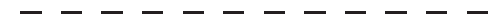
\includegraphics[scale=0.75]{interaction}
\caption{Diagrammatic representation of the interaction line.}
\label{intline}
\end{figure}

\item The cluster operators are depicted by solid horizontal lines as in Fig.~\ref{clusterline}
\begin{figure}[htp]
\centering
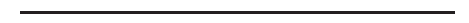
\includegraphics[scale=0.75]{cluster}
\caption{Depiction of the cluster operator.}
\label{clusterline}
\end{figure}


\item The one particle component of the Hamiltonian is represented
		by a dashed interaction line capped by an $X,$ see Fig.~\ref{hartreeX}.
\begin{figure}[htp]
\centering
\includegraphics[scale=0.75]{hartreefockop}
\caption{Depiction of the one particle component of the Hamiltonian.}
\label{hartreeX}
\end{figure}



\item Representation of the cluster operators is seen in 
Fig.~\ref{clusterdi}. In the diagram representing the $T_1$ amplitude there
is one incoming hole line and one outgoing particle line meeting at a solid
horizontal line.


\begin{figure}[htp]
\centering
\includegraphics[scale=0.5]{clusterdi}
\caption{Diagrammatic representation of the cluster operators $T_1$
and $T_2$.}
\label{clusterdi}
\end{figure}

The diagram representing $T_2$ consists of two incoming hole lines and two
outgoing particle lines. 

\item We label  particle lines with $a,b,c,d,\cdots\,.$ and all hole lines with $i,j,k,l,\cdots\,.$.

\item We sum over internal lines, all indices associated with lines that begins and ends at operator interaction lines and do not extend to infinity above or below the diagram.

\item For each hole line, multiply with a factor of -1.

\item For each loop, multiply with a factor of -1. In Fig.~\ref{loops} we have depicted the interpretations of loops in the coupled cluster diagrams. A loop is a route a long a series of directed lines that either returns to its beginning or begins at one external line and ends at another.
\begin{figure}[htp]
\centering
\includegraphics[scale=0.75]{loops}
\caption{Three different types of loops in the coupled cluster diagrams.}
\label{loops}
\end{figure}

\item For each pair of equivalent lines multiply with the factor $1/2$. An equivalent pair of lines are lines beginning at the same operator interaction line and ending at the same interaction line.

\item If there are $n$ equivalent vertices's in the diagram, multiply
with the factor $1/n!.$

\item For each pair of unique external hole or particle lines, multiply with
 the permutation operator $P(pq).$


\end{enumerate}
By using the above diagram rules it is possible to write diagrams
corresponding to the energy equation and amplitude equations. \\
Like the diagrams for the energy equation in Eq.~\eqref{lastformham}
\be
E=\bra{\Phi_0}H_N+H_NT_1+H_Nt_2+\frac{1}{2}H_NT^2_1+\dots \ket{\Phi_0}
\ee
can be evaluated with the above rules. The first term will not
contribute since the operator is normalized and therefore will
annihilate the vacuum state and give zero contribution.\\
\\
We will now study how the second term
\be
\bra{\Phi_0}H_NT_1\ket{\Phi_0},
\label{firstendi}
\ee
which may be depicted as a Feynman-Goldstone diagram.\\
Since we have the reference vacuum in both incoming and outgoing states there
should be no external lines, meaning that there should not be 
any line neither below or above the two horizontal operator 
lines. The $T_1$ operator stands to the right, and its 
corresponding interaction line should be in the bottom of 
the diagram. Only the one particle operator contributes since with a two 
particle operator it is impossible to draw a diagram with just internal 
lines, see Fig. \ref{firstenedi}. 
%Fig. (\ref{firstenedi}) shows the diagrammatic representation of
%the energy term $\bra{\Phi_0}H_NT_1\ket{\Phi_0}.$
%Eq. \eqref{firstendi}
\begin{figure}[htp]
\centering
\includegraphics[scale=0.75]{firstenedi}
\caption{Diagrammatic representation of the first term in the 
ECCSD energy equation.}
\label{firstenedi}
\end{figure}
In the second contribution,
\be
\bra{\Phi_0}H_NT_2\ket{\Phi_0},
\label{secendi}
\ee
we have the reference vacuum in both incoming and outgoing state and therefore no external lines. Since the 
cluster operator is the rightmost one, the interaction line 
representing it should again be at the bottom. However, to this 
part only the two-particle operator of the Hamiltonian is 
contributing, something which should be reflected in the 
diagram. Figure \ref{secndi} shows the diagram representing Eq.~\eqref{secendi}.
\begin{figure}[htp]
\centering
\includegraphics[scale=0.75]{secenedi}
\caption{Diagrammatic representation of the second term in the 
ECCSD energy equation.}
\label{secndi}
\end{figure}
The last part contributing to the $ECCSD$ energy equation is the
term 
\be
\frac{1}{2}\bra{\Phi_0}H_NT_1^2\ket{\Phi_0}.
\label{thirdpartendi}
\ee
The interaction lines corresponding to the two cluster operators
will again have to be drawn at the bottom of the diagram, the 
difference in this diagram, Fig.~\ref{thirdenedi}, from 
Fig.~\ref{secndi} is that the 
interaction line corresponding to the cluster operator is 
split since there are two one-excitation cluster operators to
the right in Eq.~\eqref{thirdpartendi}. 
\begin{figure}[htp]
\centering
\includegraphics[scale=0.75]{thirdenedi}
\caption{Diagrammatic representation of the last term in the 
ECCSD energy equation.}
\label{thirdenedi}
\end{figure}
We can find the $T$ amplitude diagrams by using the commutators and the above diagram rules. However it is more practical to derive the amplitude equations from the amplitude diagrams. We start by
drawing all topologically distinct diagrams with  one external hole line and one external particle line for 
the $T_1$ amplitude equation. For the $T_2$ diagrams we must consider that there are two external hole 
lines and two external particle lines.\\
\\
The first leading term 
in the equation corresponding to $T_1$ consists just of the Hamiltonian, and 
only the one particle part of it contributes. Its corresponding diagram is
depicted in Fig. \ref{firstamplt1}.  
\begin{figure}[htp]
\centering
\includegraphics[scale=0.75]{firstampl}
\caption{The diagram representing the first leading term in the
$T_1$ amplitude equation.}
\label{firstamplt1}
\end{figure} 
All diagrams contributing to the $T_1$ equation can be seen in Fig.~\ref{t1_eqn_diag}.\\
\begin{figure}[htp]
%\begin{minipage}{2in}%[t]{0.5\linewidth}
\centering
\includegraphics[scale=0.25]{t1_eqn_diag}
\caption{All diagrams contributing to the equation for solving the
$T_1$ amplitude.}
\label{t1_eqn_diag}
%\end{minipage}
\end{figure}
%\hspace{0.5cm}
%\begin{minipage}{2in}%[t]{0.5\linewidth}
In Fig.~\ref{t2_eqn_diag} we depicted all diagrams contributing to the CCD equation, while the remaining parts in a CCSD approximation are depicted in 
Fig.~\ref{t2_eqn_diag_ccsd}.  
%\end{minipage}
%\clearpage
\begin{figure}[htp]
\centering
\includegraphics[scale=0.5]{t2_eqn_diag}%{CCD_diag}
\caption{All diagrams contributing to the equation for solving the
$T_2$ amplitude in the CCD approach.}
\label{t2_eqn_diag}
\end{figure}
\begin{figure}[htp]
\centering
\includegraphics[scale=0.5]{t2_eqn_diag2}%{CCSD_diag}
\caption{The diagrams remaining in a CCSD approach to the
$T_2$ amplitude.}
\label{t2_eqn_diag_ccsd}
\end{figure}\\
%\clearpage
\\
To see the benefit with the diagrams, the $CCSD$ energy 
equation will now be computed from the diagrams. The total 
energy can be depicted as in Fig.~\ref{totenergydi}\\
\begin{figure}[htp]
\centering
\includegraphics[width=1.0\textwidth]{energy}
\caption{The diagrams representing the total $CCSD$ 
energy.}
\label{totenergydi}
\end{figure}
The way to interpret the diagrams is from the bottom to the 
upper part. The ingoing states are 
represented by a ket vector and the outgoing by the dual bra 
vector. In the first diagram in Fig.~\ref{totenergydi} the one-excitation operator line is at the bottom. We
label each internal particle and hole line and perform a sum over all hole and particle states. We have one
hole line and one loop which together contributes as $(-1)^{1+1}=1$. On top we have a one-body
interaction line. We find that the first diagram in Fig.~\ref{totenergydi} 
should be understood as
\be
\sum_{ai}f_{ia}t^a_i,
\ee
By using the above diagram 
rules to the second diagram in Fig.~\ref{totenergydi}, we find its
matrix elements to be
\be
\frac{1}{4}\sum_{ijab}v_{ijab}t^{ab}_{ij},
\ee
where $v_{ijab}=\bra{ij}v\ket{ab}.$  We have two loops and two hole lines which together contribute with the factor $1$. We have two pairs of equivalent lines which together contribute with the factor $1/4$. A factor of $1/2$ for each pair of equivalent lines. With the same reasoning we write the last
diagram in Fig.~\ref{totenergydi} as
\be
\frac{1}{2}\sum_{ijab}\bra{ij}v_N\ket{ab}t^a_it^b_j=\frac{1}{2}\sum_{ijab}v_{ijab}t^a_it^b_j.
\ee
The factor of $1/2$ appears because of two equivalent vertices.
After summing up the energy,  the total equation becomes
\be
\sum_{ia}f_{ia}t^a_i+\frac{1}{4}\sum_{ijab}v_{ijab}t^{ab}_{ij}
+\frac{1}{2}\sum_{ijab}v_{ijab}t^a_it^b_j,
\ee
which is exactly the same as the equation got by using Wick's 
theorem.\\ 

%The same reasoning as above for the energy equation can be done
%at the $CCSD$ amplitude equations. In this case one has to take
%in consideration that the states dealed with are excited states
%projected on the normaled ordered coupled cluster Hamiltonian 
%operated on the groundstate.
%
%The leading term in the $T_1$ amplitude  equation is $\bra{\Phi^a_i}H_N\ket{\Phi_0}$. Only the one particle operator is 
%contributing here, the corresponding diagram would be 
%
%\begin{figure}[htp]
%\centering
%\includegraphics{firstampl}
%\caption{The diagram representing the first leading term in the
%$T_1$ amplitude equation. The interpretation is $f_{ai}$ }
%\label{firstamplt}
%\end{figure}
%
%Converting the diagram in Fig. (\ref{firstamplt}) to an equation
%would give the result $f_{ai}.$
%
%The first leading term in the $T_2$ amplitude equation is
%$\bra{\Phi^{ab}_{ij}}H_N\ket{\Phi_0},$ only the two-particle 
%operator is contributing to this part and the diagram is as is 
%shown in Fig. (\ref{secamplt})
%
%\begin{figure}[htp]
%\centering
%\includegraphics{secampl}
%\caption{The diagram representing the first leading term in the
%$T_2$ amplitude equation. It is representing the equation 
%$V_{ijab}$ }
%\label{secamplt}
%\end{figure}
%
%The matrix element, Fig(\ref{secamplt}), is $\bra{ab}V\ket{ij}.$
%\clearpage
\section{Computation of the equations}
\label{compofccsd}

This section will treat the computational approach for solving the amplitude
equations as Eqs.~\eqref{firstamplitude} and \eqref{secondamplitude}.
It is not always clear how one should approach the equations. 
A first approach could be to rearrange the equations to provide a more handy form. As an example the first few terms of Eq. \eqref{firstamplitude}, could be written as
\be
0=f_{ai}+f_{aa}t^a_i-f_{ii}t^a_i+\sum_c(1-\delta_{ca})f_{ac}t^c_i-\sum_k (1-\delta_{ik})f_{ik}t^a_k+\cdots
\label{firstfirstampl}
\ee
By defining 
\be
D^a_i=f_{ii}-f_{aa}
\ee
we rewrite Eq.~\eqref{firstfirstampl} as 
\be
D^a_it^a_i=f_{ai}+\sum_c(1-\delta_{ca})f_{ac}t^c_i-\sum_k(1-\delta_{ik})f_{ik}t^a_k+\cdots.
\ee
By also defining 
\be
D^{ab}_{ij}=f_{ii}+f_{jj}-f_{aa}-f_{bb}
\ee
the $T_2$ amplitude can be rewritten as
\be
D^{ab}_{ij}t^{ab}_{ij}=\bra{ab}v\ket{ij}+P(ab)\sum_c(1-\delta_{bc})f_{bc}t^{ac}_{ij}-P(ij)\sum_{k}(1-\delta_{kj})f_{kj}t^{ab}_{ik}+\cdots
\ee
The equations above have to be solved iteratively. A starting point for $t^a_i$ and $t^{ab}_{ij}$ may be obtained by setting all of the amplitudes on the right-hand side to zero. The initial guess for the amplitudes are then
\be
t^a_i=f_{ai}/D^a_i,
\ee 
for the $T_1$ amplitude and 
\be
t^{ab}_{ij}=\bra{ab}v\ket{ij}/D^{ab}_{ij}
\ee
for the $T_2$ amplitude.\\
These initial guesses have to be inserted on the right-hand side of the 
equations and then subsequently used to obtain new 
amplitudes. This process is continued until an explicit convergence is 
reached.\\
\\
In momentum space and a plane wave basis in addition to the sum over single-particle states in the energy and amplitude equations, we will
also have to integrate over the momentum for each single-particle state. Holes have momentum less than the 
Fermi momentum $k_f$, while particles have momentum greater than $k_f$.\\
\\
The single-particle functions $\varphi$ are defined as plane-waves
\beq
\varphi=\frac{1}{\sqrt{\Omega}}e^{i\bold k\bold r},
\eeq
where the volume, $\Omega$ is infinite, $k$ denotes the principal wave-number and $r$ the radial coordinate.
When we calculate interactions it is convenient to do a so-called partial wave-expansion.
We expand the exponential as a sum of Legendre polynomials and spherical Bessel functions
\beq
e^{ikr}=\sum_{l=0}^\infty(2l+1)i^lj_l(kr)P_l(\Omega_{k,r}),
\eeq
where the spherical Bessel functions $j_l(kr)$ depends on the radial part of the momentum and position vector, see appendix \ref{app:leg} and \ref{app:bess} for details about the functions. The Legendre polynomials $P_l$ depends on 
$\Omega_{k,r}=\bold k\cdot \bold r/(|k||r|)$, which is the cosine angle between $\bold k$ and $\bold r$. The sum goes over orbital momentum $l$.\\ 
\\
We saw in Eqs.~\eqref{firstamplitude} and \eqref{secondamplitude} that there
are many diagrams contributing to the amplitude equations, as many diagrams
as terms in the equations. It requires a lot of time computing all these
diagrams separately, therefore it is wise to 
factorize the diagrams. This can be done, since the coupled cluster diagrams do not have any denominators in their's expressions,
in contrast to the diagrams in perturbation theory. 
Instead of computing the same factors several times, we compute it once and
multiply it with the corresponding terms, as explained by Ref.~\cite{bartlett:291}. In this work the factorization used is the same as the one used by Ref.~\cite{hagen:034302}.

\section{Further analysis of the coupled cluster method} In the section on
perturbation theory we derived the diagram rules and draw diagrams
up to third order.  In section \ref{compofccsd} we showed how to solve the CCSD equations. With an initial guess for the $T_2$ amplitude as
\be\frac{\bra{ab}v\ket{ij}}{f_{ij}-f_{ab}}\ee 
and insert it in the CCSD energy equation gives us
\be
E_{T_2}= \frac{1}{4}\sum_{\substack{i,j \\a,b}} v_{ijab}t^{ab}_{ij}=\frac{1}{4}\sum_{\substack{i,j \\a,b}}\frac{\bra{ij}v\ket{ab}\bra{ab}v\ket{ij}}{f_{ij}-f_{ab}},
\ee
which is exactly the same expression as the second order contribution to the energy in perturbation theory. 
By doing more of the iterations, the coupled cluster method will also include diagrams from third and fourth
order in perturbation theory.\\ % We see that
%there is a fine connection between the coupled cluster calculations and calculations with perturbation theory.\\
\\
A convenient property of the coupled cluster method is that it is size
consistent and size extensive. By size consistent we mean that computing the
energy of two nuclei with an infinite distance between them is just to compute
the two energies separately. As an example we consider two
nuclei, $A$ and $B.$
\be
\begin{split}
&\ket{\Phi_0} = \ket{\Phi^A_0}\ket{\Phi^B_0}\\
&e^T\ket{\Phi_0}=e^{T_A+T_B}\ket{\Phi^A_0}\ket{\Phi^B_0}=e^{T_A}\ket{\Phi^A_0}e^{T_B}\ket{\Phi^B_0}.\\
\end{split}
\ee
With the Hamiltonian on the form $H=H_A + H_B$ the energy of the combined system  sums up to  
\be
E_{CC}= E^A_{CC} + E^B_{CC}.
\ee
With size extensive means that the energy is linearly dependent on the number of particles present. 




















 % coupled.tex
\clearemptydoublepage
%\part{Implementation}
\include{chapter8} % coupled.tex
\clearemptydoublepage
\chapter{Calculations and results}

The hardest task in doing the calculations was to write out the matrix
elements to be read by another program that performs the coupled
cluster calculations.% As we wanted to make as good a calculation as possible we
%tried to make the model space as huge as possible.% We soon realized that it
%would take to much time.\\
\\
When operating in a plane wave basis we have both the mesh points for the numerical
integration and the orbital angular momentum number $l$  to consider, since we use a
partial wave expansion of the wave function in a plane wave basis. 
The idea was to fix the maximum value of $l$ to six, and
number of mesh points to 12. However it seemed that the maximum orbital angular
momentum number had to be lowered to finish the thesis in time.\\% Of course the
%precision would be much better with both increasing the orbital angular
%momentum number and mesh points and it is assumed that the values predicted would have
%improved.\\
\\
As we are doing the calculations with just two-body forces, and in a plane wave
basis, the Hamiltonian is composed of the kinetic energy  and a
two-body interaction, defined as
\begin{equation*}
		\begin{split}
				&H=\sum_{i=0}^A\frac{1}{2m}\bra{i}k^2\ket{i}a^\dagger_ia_i + \frac{1}{2}\sum_{ijkl}\bra{ij}v\ket{kl}a^\dagger_ia^\dagger_ja_la_k.
		\end{split}
\end{equation*}
When we integrate over momentum we are left with an undefined volume term
$\Omega$. We can overcome this problem by dividing with the number of particles. 
Technically this is done by dividing each energy term by the volume, $\Omega$, and 
the density, $\rho$, defined in Eq.~(\eqref{eq:density}). We obtain then the expression
\begin{equation*}
		\begin{split}
			&	 \sum_{jt_z} (2j+1)\int _0^{k_f}\frac{k^4}{2\pi^2}dk\frac{1}{2m_N\rho}+\\
			&	\sum_{\substack{j_1l_l1t_{z_1}\\j_2l_2t_{z_2}}}\sum_{\substack{j_3l_3t_{z_3}\\j_4l_4t_{z_4}}}(2J+1)\int \frac{d^3k_1 d^3k_2 d^3k_3 d^3k_4}{(2\pi)^{12}\rho}\bra{j_1l_1k_1t_{z_1}j_2l_2k_2t_{z_2}JT_z}v
				\ket{j_3l_3k_3t_{z_3}j_4l_4k_4t_{z_4}JT_z}.
		\end{split}
\end{equation*}
In a numerical calculation the integrals over $k$ are approximated by finite sums over the number
of mesh points $N$ 
\begin{equation*}
		\int f(k)k^2dk \rightarrow \sum_i^N f(k_i)k^2_i\omega_i,
\end{equation*}
where $k_i$ and $\omega_i$ are the integration points (mesh points) and integration weights, respectively.
In performing the integrals numerically we employed Gaussian quadrature 
(with Legendre polynomials), for details see \cite{compphys-mhjensen}.\\
\\
The nuclear interaction model used is the chiral N$^3$LO version of Entem and Machleidt 
\cite{entem-2003-68} with cutoff, 
$\Lambda=500$ MeV. We
renormalized the $N^3LO$ potential using the similarity transformation in momentum space described earlier. This is interaction is labelled $V_{low-k}$ with model spaces defined by the different values of the cutoff  $\lambda$. We have employed the following values of the cutoff
2.1 $\mbox{fm}^{-1}$, 2.2 fm$^{-1}$ and 2.5 fm$^{-1}$.\\
\\
%%sjekk
Most nuclear matter calculations have been done with a
perturbational approach, starting with renormalizing the potential 
with for example a similarity transformation method in momentum space, yielding the so-called  
$V_{low-k}$ 
renormalization scheme. The Brueckner $G$-matrix approach is also an often used as starting points for nuclear matter computations. It is a way to circumvent
the strictly unperturbative part of the nuclear interactions, it is briefly described
in appendix \ref{bgm}.  
\\
\section{The programs}

Two separate programs were used, one which calculates the interaction elements in
the laboratory frame and then the other program that performs the coupled cluster
computations. As said above the hardest task was to compute the interactions. This part is rather
time-consuming  due teh computation of the vector-bracket coefficients.  In order to improve
the efficiency it had to be parallelized. It was not so difficult to parallellize the program since one interaction element does not depend on the other elements. 
The computation of the interaction elements was 
spread evenly on different processes.  
The pseudo-code below shows how a for-loop was parallelized.
\begin{algorithm}
\begin{algorithmic}
		\FOR{$i$= iam+1, n, numprocs}
         \STATE   some code
        \ENDFOR
\end{algorithmic}
\end{algorithm}\\
Complications
arose when the interaction elements were written to the file to be read by the coupled cluster
program.  The easiest way was to let each process write their matrix elements
to their own file and then concatenate the files to one. This is a rather fast
process but it generates a lots of files and is not always easily implemented on the supercomputing
clusters (Titan@uio.no and Hexagon@uib.no) which we had access to in this thesis work.
What was done was to let each process store their interaction elements in
an array which was sent to the master node, which then writes them to file. This
is a rather tedious and slow process and it is not recommended.\\
\\
A better method
would be to use the MPI I/O functions, which let the processes write to the
same file. The complications which made us avoid the MPI I/O method was that we
needed to know both the total file size and the size each processes write.
Because of the bracket transformations it was difficult to 
know how much each process would need to
write. We came to the conclusion that if we gave the processes a too huge size
of the file than necessary, it could generate blank lines, which may get problematic when reading it. Another MPI tool to use is NETCDF4/HDF5, however with this it was difficult to write the matrix elements in the form the coupled cluster
program demands.\\
\\
The coupled cluster program used, was originally written in a harmonic oscillator basis. 
Some minor changes in how the program reads the interaction elements 
had to be done in order  to make the coupled cluster program work in a plane wave basis as well. 
In order not to change  the program too much the matrix elements to be read were already multiplied with the mesh points and weights for the integrations
\begin{equation*}
		\begin{split}
             &\bra{l_1j_1k_2l_2k_2JT_z}v\ket{l_3j_3k_3l_4j_4k_4JT_z}\\
             & \rightarrow \bra{l_1j_1k_1l_2j_2k_2JT_z}v\ket{l_3j_3k_3l_4j_4k_4JT_z}k_1k_2k_3k_4\sqrt{w_1w_2w_3w_4}.
        \end{split}
\end{equation*}
Then the only thing needed was to multiply with the factor $1/(2\pi)^2$  for
each integration variable and keep in mind that nothing should be divided by
the weights and mesh points when solving for the cluster amplitudes. 

\clearpage


\section{Results and conclusion}

The aim of the thesis was to calculate the binding energy of symmetric nuclear
matter and obtain an equation of state of pure neutron matter with the coupled
cluster method. As this was done in a plane wave basis, we had to do an
integration over momentum, $k$, in the region where $k\in[0,\infty]$.
Numerically this is accomplished by a tangential mapping. As the
renormalization scheme V$_{low-k}$ was used, the problem is projected to
a smaller space by defining $k\in[0,\lambda]$, where $\lambda$ usually ranges from 2
fm$^{-1}$ to 3 fm$^{-1}$. The tangential projection procedure was omitted since
the meshpoints were projected onto the new interval $k\in[0,\lambda]$.\\
\\
In chapter \ref{ch:coupled} we saw that when doing coupled cluster calculation
we have to make a distinction between particles and holes. In chapter
\ref{chapsecondq} we defined holes as particles inside the Fermi sphere and
particles to be outside. The radius of the Fermi sphere was set to be $k_f$
where $k_f$ ranges from 1.2 fm$^{-1}$ to 1.9 fm$^{-1}$. All single-particle
states with a momentum below or equal $k_f$ are to be holes and those with a
momentum greater than $k_f$ were defined as particles.\\
\\
In Figs.~\ref{fig:hf21}-\ref{fig:hf23} we present the first-order energies for orbital angular momentum, $l$, values
truncated at four and six.  The saturation density remains more or less constant
for both $l$-values at 1.75 fm$^{-1}$, which is greater than the experimental
value at 1.42 fm$^{-1}$. The binding energy, approximately $3$MeV, are way too low for orbital angular momentum
truncated at 4, compared to the experimental value, 16 MeV. For $\lambda=2.5$
fm$^{-1}$ the first order approximation failed to give a minimum.
An interesting observation is that the
cutoff  $\lambda=2.1$ fm$^{-1}$ gives a higher binding energy (lower minimum) than the cutoff
on 2.2 fm$^{-1}$. This is because the  interaction elements with lower $\lambda$
have higher absolute values. This will of course have an effect on the coupled cluster
computations as well. It is believed that three-body forces may correct for the dependency on the cutoff.\\
\\
The first-order calculations with angular momentum truncated at $l=6$ and 
$\lambda=2.2$ almost reproduce the experimental binding energy, but with a 
higher cutoff the interaction elements get smaller and fail to reproduce the 
experimental binding energy. Coupled cluster computation on $l=6$ were not 
completed since they were very time consuming and required too much memory to be run on Hexagon@uib.no.\\
\\
In the case of pure neutron matter the equation of state is almost 
constant as function of the cutoff, as can be seen in Figs.~\ref{fig:first_neutron_l4} and \ref{fig:ccm_net_4_21}.\\
\\
In Figs.~\ref{fig:ccm_nucl_4_21} and \ref{fig:ccm_net_4_21} we present coupled cluster calculations for symmetric nuclear matter and pure neutron matter, respectively.
We see that it is almost identical to the first-order energies.% for first order
%
\begin{table}
		\centering
		\begin{tabular}{|c|c|c|c|c|c|}
				\hline
				\multicolumn{3}{|c|}{$\lambda=2.1$ fm$^{-1}$}& \multicolumn{3}{c|}{$l_{\mbox{max}}=4$ }\\
				\hline
				$k_f$ & Total energy & $\sum_{ai}f_{ai}t^a_i$ & $\sum_{abij}v_{abij}t^a_it^b_j$ & $\sum_{abij}v_{abij}t^{ab}_{ij}$ & Total correction\\
				\hline
				1.2 & 3.787507 & -0.030488 & -0.000117 & -0.058656 & -0.089261  \\
				\hline
				1.4 & 3.82199 &  -0.030239 & -0.000889 & -0.145316 & -0.175644\\
				\hline
				1.6 & -2.071725 & -0.057642 & -0.000140 & -0.113498 & -0.171280 \\
				\hline
				1.8 & -4.307874 & -0.117001 & -0.000423 & -0.058656 & 0.176080 \\
				\hline
				1.9 & 0.215606 & -0.05693 & -0.000129 & -0.032594 & -0.089660 \\
				\hline
		%		\hline
				\multicolumn{3}{|c|}{$\lambda=2.2$ fm$^{-1}$}& \multicolumn{3}{c|}{$l_{\mbox{max}}=4$ }\\
				\hline
				$k_f$ & Total energy & $\sum_{ai}f_{ai}t^a_i$ & $\sum_{abij}v_{abij}t^a_it^b_j$ & $\sum_{abij}v_{abij}t^{ab}_{ij}$ & Total correction\\
				\hline
				1.2 & 2.856008 & -0.025748 & -0.000100 & -0.153787 & -0.179635\\
				\hline
				1.4 & 3.664643 & -0.026888 & -0.000006 & -0.175784 & -0.202737\\
			    \hline
				1.6 & 1.429075 & -0.075102 & -0.000432 & -0.184876 & -0.260410\\
				\hline
				1.7 &-4.663540 & -0.186931 & -0.002106 & -0.169220 & -0.358257\\
				\hline
				\multicolumn{3}{|c|}{$\lambda=2.5$ fm$^{-1}$}& \multicolumn{3}{c|}{$l_{\mbox{max}}=4$ }\\
				\hline
				1.4 & 6.426474 & 0.001282 & 0.000037 & -0.322986 & -0.321667\\
				\hline
			%	\multicolumn{3}{|c|}{$\lambda=3.0$ fm$^{-1}$}& \multicolumn{3}{c|}{$l_{\mbox{max}}=4$ }\\
			%	\hline
			%	\multicolumn{3}{|c|}{$\lambda=2.2$ fm$^{-1}$}& \multicolumn{3}{c|}{$l_{\mbox{max}}=6$ }\\
			%	\hline
		\end{tabular}
		\caption{Energies and correction to the first order energy for different values of $\lambda$ and $k_f$. All energies are in MeV}
		\label{tab:korreksjoner}
\end{table}
%it seems that the cluster amplitudes are almost zero, meaning that the state $\Psi$ is almost identical to the state $\Phi_0$. 
\begin{figure}[htpb]
		\input{symmetric_hfl4_2_1}
		\caption{First-order energy for orbital angular momentum truncated at $l=4$, 
and cutoffs  $\lambda=2.1$fm$^{-1}$, $\lambda=2.2$fm$^{-1}$ and $\lambda=2.5$ fm$^{-1}$.}
		\label{fig:hf21}
\end{figure}
%\begin{figure}[htpb]
%		\input{symmetric_hfl4_2_2}
%		\caption{Hartree-Fock energy for orbital momentum truncated at 4, and a cutoff $\lambda=2.2$.}
%		\label{fig:hf22}
%\end{figure}
\begin{figure}[htpb]
		% GNUPLOT: LaTeX picture with Postscript
\begingroup
  \makeatletter
  \providecommand\color[2][]{%
    \GenericError{(gnuplot) \space\space\space\@spaces}{%
      Package color not loaded in conjunction with
      terminal option `colourtext'%
    }{See the gnuplot documentation for explanation.%
    }{Either use 'blacktext' in gnuplot or load the package
      color.sty in LaTeX.}%
    \renewcommand\color[2][]{}%
  }%
  \providecommand\includegraphics[2][]{%
    \GenericError{(gnuplot) \space\space\space\@spaces}{%
      Package graphicx or graphics not loaded%
    }{See the gnuplot documentation for explanation.%
    }{The gnuplot epslatex terminal needs graphicx.sty or graphics.sty.}%
    \renewcommand\includegraphics[2][]{}%
  }%
  \providecommand\rotatebox[2]{#2}%
  \@ifundefined{ifGPcolor}{%
    \newif\ifGPcolor
    \GPcolortrue
  }{}%
  \@ifundefined{ifGPblacktext}{%
    \newif\ifGPblacktext
    \GPblacktexttrue
  }{}%
  % define a \g@addto@macro without @ in the name:
  \let\gplgaddtomacro\g@addto@macro
  % define empty templates for all commands taking text:
  \gdef\gplbacktext{}%
  \gdef\gplfronttext{}%
  \makeatother
  \ifGPblacktext
    % no textcolor at all
    \def\colorrgb#1{}%
    \def\colorgray#1{}%
  \else
    % gray or color?
    \ifGPcolor
      \def\colorrgb#1{\color[rgb]{#1}}%
      \def\colorgray#1{\color[gray]{#1}}%
      \expandafter\def\csname LTw\endcsname{\color{white}}%
      \expandafter\def\csname LTb\endcsname{\color{black}}%
      \expandafter\def\csname LTa\endcsname{\color{black}}%
      \expandafter\def\csname LT0\endcsname{\color[rgb]{1,0,0}}%
      \expandafter\def\csname LT1\endcsname{\color[rgb]{0,1,0}}%
      \expandafter\def\csname LT2\endcsname{\color[rgb]{0,0,1}}%
      \expandafter\def\csname LT3\endcsname{\color[rgb]{1,0,1}}%
      \expandafter\def\csname LT4\endcsname{\color[rgb]{0,1,1}}%
      \expandafter\def\csname LT5\endcsname{\color[rgb]{1,1,0}}%
      \expandafter\def\csname LT6\endcsname{\color[rgb]{0,0,0}}%
      \expandafter\def\csname LT7\endcsname{\color[rgb]{1,0.3,0}}%
      \expandafter\def\csname LT8\endcsname{\color[rgb]{0.5,0.5,0.5}}%
    \else
      % gray
      \def\colorrgb#1{\color{black}}%
      \def\colorgray#1{\color[gray]{#1}}%
      \expandafter\def\csname LTw\endcsname{\color{white}}%
      \expandafter\def\csname LTb\endcsname{\color{black}}%
      \expandafter\def\csname LTa\endcsname{\color{black}}%
      \expandafter\def\csname LT0\endcsname{\color{black}}%
      \expandafter\def\csname LT1\endcsname{\color{black}}%
      \expandafter\def\csname LT2\endcsname{\color{black}}%
      \expandafter\def\csname LT3\endcsname{\color{black}}%
      \expandafter\def\csname LT4\endcsname{\color{black}}%
      \expandafter\def\csname LT5\endcsname{\color{black}}%
      \expandafter\def\csname LT6\endcsname{\color{black}}%
      \expandafter\def\csname LT7\endcsname{\color{black}}%
      \expandafter\def\csname LT8\endcsname{\color{black}}%
    \fi
  \fi
  \setlength{\unitlength}{0.0500bp}%
  \begin{picture}(7200.00,5040.00)%
    \gplgaddtomacro\gplbacktext{%
      \csname LTb\endcsname%
      \put(1122,660){\makebox(0,0)[r]{\strut{}$-25$}}%
      \put(1122,1280){\makebox(0,0)[r]{\strut{}$-20$}}%
      \put(1122,1900){\makebox(0,0)[r]{\strut{}$-15$}}%
      \put(1122,2520){\makebox(0,0)[r]{\strut{}$-10$}}%
      \put(1122,3140){\makebox(0,0)[r]{\strut{}$-5$}}%
      \put(1122,3760){\makebox(0,0)[r]{\strut{}$0$}}%
      \put(1122,4380){\makebox(0,0)[r]{\strut{}$5$}}%
      \put(1254,440){\makebox(0,0){\strut{}$1.2$}}%
      \put(1951,440){\makebox(0,0){\strut{}$1.3$}}%
      \put(2647,440){\makebox(0,0){\strut{}$1.4$}}%
      \put(3344,440){\makebox(0,0){\strut{}$1.5$}}%
      \put(4040,440){\makebox(0,0){\strut{}$1.6$}}%
      \put(4737,440){\makebox(0,0){\strut{}$1.7$}}%
      \put(5433,440){\makebox(0,0){\strut{}$1.8$}}%
      \put(6130,440){\makebox(0,0){\strut{}$1.9$}}%
      \put(6826,440){\makebox(0,0){\strut{}$2$}}%
      \put(220,2520){\rotatebox{90}{\makebox(0,0){\strut{}E/A [MeV]}}}%
      \put(4040,110){\makebox(0,0){\strut{}$k_f$}}%
      \put(4040,4710){\makebox(0,0){\strut{}First order energies for symmetric nuclear matter, $l=6$.}}%
    }%
    \gplgaddtomacro\gplfronttext{%
      \csname LTb\endcsname%
      \put(5839,4207){\makebox(0,0)[r]{\strut{}$\lambda=2.2$ fm$^{-1}$}}%
      \csname LTb\endcsname%
      \put(5839,3987){\makebox(0,0)[r]{\strut{}$\lambda=2.1$ fm$^{-1}$}}%
      \csname LTb\endcsname%
      \put(5839,3767){\makebox(0,0)[r]{\strut{}$\lambda=2.5$ fm$^{-1}$}}%
    }%
    \gplbacktext
    \put(0,0){\includegraphics{symmetric_hfl6_2_2}}%
    \gplfronttext
  \end{picture}%
\endgroup

		\caption{First-order corrections to energy per particle, with the orbital angular momentum truncated at $l=6$ and momentum cutoff $\lambda=2.2$.}
		\label{fig:hf23}
\end{figure}
\begin{figure}
% GNUPLOT: LaTeX picture with Postscript
\begingroup
  \makeatletter
  \providecommand\color[2][]{%
    \GenericError{(gnuplot) \space\space\space\@spaces}{%
      Package color not loaded in conjunction with
      terminal option `colourtext'%
    }{See the gnuplot documentation for explanation.%
    }{Either use 'blacktext' in gnuplot or load the package
      color.sty in LaTeX.}%
    \renewcommand\color[2][]{}%
  }%
  \providecommand\includegraphics[2][]{%
    \GenericError{(gnuplot) \space\space\space\@spaces}{%
      Package graphicx or graphics not loaded%
    }{See the gnuplot documentation for explanation.%
    }{The gnuplot epslatex terminal needs graphicx.sty or graphics.sty.}%
    \renewcommand\includegraphics[2][]{}%
  }%
  \providecommand\rotatebox[2]{#2}%
  \@ifundefined{ifGPcolor}{%
    \newif\ifGPcolor
    \GPcolortrue
  }{}%
  \@ifundefined{ifGPblacktext}{%
    \newif\ifGPblacktext
    \GPblacktexttrue
  }{}%
  % define a \g@addto@macro without @ in the name:
  \let\gplgaddtomacro\g@addto@macro
  % define empty templates for all commands taking text:
  \gdef\gplbacktext{}%
  \gdef\gplfronttext{}%
  \makeatother
  \ifGPblacktext
    % no textcolor at all
    \def\colorrgb#1{}%
    \def\colorgray#1{}%
  \else
    % gray or color?
    \ifGPcolor
      \def\colorrgb#1{\color[rgb]{#1}}%
      \def\colorgray#1{\color[gray]{#1}}%
      \expandafter\def\csname LTw\endcsname{\color{white}}%
      \expandafter\def\csname LTb\endcsname{\color{black}}%
      \expandafter\def\csname LTa\endcsname{\color{black}}%
      \expandafter\def\csname LT0\endcsname{\color[rgb]{1,0,0}}%
      \expandafter\def\csname LT1\endcsname{\color[rgb]{0,1,0}}%
      \expandafter\def\csname LT2\endcsname{\color[rgb]{0,0,1}}%
      \expandafter\def\csname LT3\endcsname{\color[rgb]{1,0,1}}%
      \expandafter\def\csname LT4\endcsname{\color[rgb]{0,1,1}}%
      \expandafter\def\csname LT5\endcsname{\color[rgb]{1,1,0}}%
      \expandafter\def\csname LT6\endcsname{\color[rgb]{0,0,0}}%
      \expandafter\def\csname LT7\endcsname{\color[rgb]{1,0.3,0}}%
      \expandafter\def\csname LT8\endcsname{\color[rgb]{0.5,0.5,0.5}}%
    \else
      % gray
      \def\colorrgb#1{\color{black}}%
      \def\colorgray#1{\color[gray]{#1}}%
      \expandafter\def\csname LTw\endcsname{\color{white}}%
      \expandafter\def\csname LTb\endcsname{\color{black}}%
      \expandafter\def\csname LTa\endcsname{\color{black}}%
      \expandafter\def\csname LT0\endcsname{\color{black}}%
      \expandafter\def\csname LT1\endcsname{\color{black}}%
      \expandafter\def\csname LT2\endcsname{\color{black}}%
      \expandafter\def\csname LT3\endcsname{\color{black}}%
      \expandafter\def\csname LT4\endcsname{\color{black}}%
      \expandafter\def\csname LT5\endcsname{\color{black}}%
      \expandafter\def\csname LT6\endcsname{\color{black}}%
      \expandafter\def\csname LT7\endcsname{\color{black}}%
      \expandafter\def\csname LT8\endcsname{\color{black}}%
    \fi
  \fi
  \setlength{\unitlength}{0.0500bp}%
  \begin{picture}(7200.00,5040.00)%
    \gplgaddtomacro\gplbacktext{%
      \csname LTb\endcsname%
      \put(990,660){\makebox(0,0)[r]{\strut{}$-5$}}%
      \put(990,1117){\makebox(0,0)[r]{\strut{}$-4$}}%
      \put(990,1575){\makebox(0,0)[r]{\strut{}$-3$}}%
      \put(990,2032){\makebox(0,0)[r]{\strut{}$-2$}}%
      \put(990,2489){\makebox(0,0)[r]{\strut{}$-1$}}%
      \put(990,2947){\makebox(0,0)[r]{\strut{}$0$}}%
      \put(990,3404){\makebox(0,0)[r]{\strut{}$1$}}%
      \put(990,3861){\makebox(0,0)[r]{\strut{}$2$}}%
      \put(990,4319){\makebox(0,0)[r]{\strut{}$3$}}%
      \put(990,4776){\makebox(0,0)[r]{\strut{}$4$}}%
      \put(1122,440){\makebox(0,0){\strut{}$1.2$}}%
      \put(1835,440){\makebox(0,0){\strut{}$1.3$}}%
      \put(2548,440){\makebox(0,0){\strut{}$1.4$}}%
      \put(3261,440){\makebox(0,0){\strut{}$1.5$}}%
      \put(3974,440){\makebox(0,0){\strut{}$1.6$}}%
      \put(4687,440){\makebox(0,0){\strut{}$1.7$}}%
      \put(5400,440){\makebox(0,0){\strut{}$1.8$}}%
      \put(6113,440){\makebox(0,0){\strut{}$1.9$}}%
      \put(6826,440){\makebox(0,0){\strut{}$2$}}%
      \put(220,2718){\rotatebox{90}{\makebox(0,0){\strut{}E/A [MeV]}}}%
      \put(3974,110){\makebox(0,0){\strut{}$k_f$ [fm$^{-1}$]}}%
    }%
    \gplgaddtomacro\gplfronttext{%
      \csname LTb\endcsname%
      \put(6339,4603){\makebox(0,0)[r]{\strut{}E/A for symmetric nuclear matter, l=4 $\lambda=2.1$, fm$^{-1}$}}%
    }%
    \gplbacktext
    \put(0,0){\includegraphics{nuclearmatterl_4_2_1}}%
    \gplfronttext
  \end{picture}%
\endgroup

\caption{Coupled cluster calculations on nuclear matter, with $l=4$ and momentum cutoff $\lambda=2.1$ fm$^{-1}$.}
\label{fig:ccm_nucl_4_21}
\end{figure}
\begin{figure}
\input{firstpureneutron_l4.tex}
\caption{First order equation of state of pure neutron matter with momentum cutoff, $\lambda=2.1$ fm$^{-1}$, $\lambda=2.2$~fm$^{-1}$~and $\lambda=2.5$~fm$^{-1}$.}
\label{fig:first_neutron_l4}
\end{figure}
\begin{figure}
\input{firstpureneutron_l6.tex}
\caption{First order equation of state of pure neutron matter with momentum cutoff $\lambda=2.2$~fm$^{-1}$~and orbital momentum truncated at 6.}
\label{fig:first_neutron_l6}
\end{figure}
%
\begin{figure}
\input{neutronmatterl_4.tex}
\caption{Coupled cluster calculations of pure neutron matter with momentum cutoff $\lambda=2.1$ fm$^{-1}$ and orbital angular momentum $l=4$.}
\label{fig:ccm_net_4_21}
\end{figure}



\subsection{Conclusion}

We can affirm that it is possible to perform coupled cluster calculations on 
nuclear matter and we have obtained an explicit convergence at least for the cutoff 
$\lambda=2.1$ fm$^{-1}$. For the cases without convergence as for 
$k_f=1.8$ fm$^{-1}$ with $\lambda=2.2$ fm$^{-1}$, $\lambda=2.5$ fm$^{-1}$ and 
$\lambda=3.0$ fm$^{-1}$ may be as a consequence of the primitive linear iteration scheme.  
As expected the convergence is faster for a smaller cutoff. This is due to the fact that
with a larger cutoff we expect more contributions from intermediate particle-particle states, as
can be seen from table \ref{tab:korreksjoner}. The model space is smaller and we have fewer particle states with small cutoffs.
However, we must admit that some of the results were not as expected, the corrections to the
first-order energy were expected to be higher, and we also notice that it seems
that the first-order energy blows up by including more orbital angular
momenta in the laboratory system. \\
\\
From Fig.~\ref{fig:hf21} we see that in the nuclear matter case the energy density depends 
strongly 
on choice of cutoff. We do not think it is fair to favor one cutoff over another, even if a cutoff reproduces the experimental value. %it is not
%fair to state that one cutoff is more correct than another. 
It may seem 
that we need a better understanding of the nuclear interactions. In Ref.~\cite{inmedium} they claim that most of the theoretical calculations on the binding energy of nuclear
matter  overbind the system up to 25\%, however some calculations also underbind
the system, which may indicate a lack of understanding the nucleon-nucleon interactions.
We also observe that the corrections to the energy is higher for a larger cutoff
$\lambda$. This may indicate that the intermediate states contribute more. 
We ''lose'' physical correlations when the cutoff is lowered.\\ 
\\
An improvement to the project and the
calculations could be to include relativistic effects and three-body interactions. The latter 
are believed to be necessary in nuclear matter and structure calculations. It could be 
convenient to make the coupled cluster program more efficient. The interaction 
files are huge and require much memory when the program stores the interactions
in arrays.   
 % coupled.tex
\clearemptydoublepage
%\chapter{The calculations} 
%!!!!!!!!!!!!!!!!!!Finn et bedre navn p\aa \, kapitlet!!!!!!!!!!!!!!!!!!!!!!!!!!!  
%\\ 
\section{The matrix elements}
The matrix elements used in the coupled cluster approximation was ordinarily given in an oscillator basis, but
transformed into a planewave basis. The general method to transform from one basis to another is by projecting the basis we want on an orthogonal and 
complete basis

\be
\ket{\alpha}=\sum_a\ket{a}\braket{a}{\alpha}.
\label{transform}
\ee

What we need is the projection of $\bra{a}$ on $\ket{\alpha}$. If we know the matrix elements of the basis $a$ and the operator $O$, then we can find the
matrix elements of the basis $\alpha$ and $O$ by projecting the complete orthonormal basis $a$ on it. 

\be
\bra{\alpha}O\ket{\alpha'}=\sum_{a,a'}\braket{\alpha}{a}\bra{a}O\ket{a'}\braket{a'}{\alpha'}
\ee


If our set of orthonormal basis states is a continuous and infinite one, the sum gets replaced by an integral. See for example Ref. Ref. \cite{gamow}.
If our operator $O$ is a twoparticle operator, our twoparticle overlap integrals read 

\be
\braket{ab}{\alpha \beta}= \frac{\braket{a}{\alpha}\braket{b}{\beta}-(-1)^{J-j_\alpha-j_\beta}\braket{a}{\beta}\braket{b}{\alpha} }{\sqrt{(1+\delta_{ab})(1+\delta_{\alpha\beta})} }
\ee

If the two particles are identical, that is proton-proton or neutron-neutron. In the proton-neutron case it reads

\be
\braket{ab}{\alpha\beta}=\braket{a}{\alpha}\braket{b}{\beta}.
\label{twopartoverlap}
\ee

With the Eqs. (\ref{transform} - \ref{twopartoverlap}), it is straightforward to make the transformations from an oscillator basis to a planewave basis. 

\be
\ket{k_a l_a j_a k_b l_b j_b J T_z} = \sum_{n_a n_b} \braket{n_a l_a j_a n_b l_b j_b J T_z}{k_a l_a j_a k_b l_b j_b J T_z}\ket{n_a l_a j_a n_b l_b j_b J T_z}
\ee
 
The task gets down to compute the twoparticle overlap $\braket{n_a l_a j_a n_b l_b j_b J T_z}{k_a l_a j_a k_b l_b j_b J T_z}$. The way to compute this relation is to look at the reverse transformation,

\be
\ket{n_a l_a j_a n_b l_b j_b J T_z}= \int k_a^2 \int k_b^2 \braket{k_a l_a j_a k_b l_b j_b J T_z}{n_a l_a j_a n_b l_b j_b J T_z}\ket{k_a l_a j_a k_b l_b j_b J T_z}dk_adk_b.
\label{transformation}
\ee
Which is nothing more than

\be
\int k_a^2 \int k_b^2 R_{n_al_a}(k_a)R_{n_bl_b}(k_b)\ket{k_a l_a j_a k_b l_b j_b J T_z}dk_adk_b.
\ee

Now, if we project the state $\bra{k'_a l'_a j'_a k'_b l'_b j'_b J'T'_z}$ on Eq. \eqref{transformation} 
we will find the expression for the transformation bracket.

\be
\begin{split}
& \braket{k'_a l'_a j'_a k'_b l'_b j'_b J'T'_z}{n_a l_a j_a n_b l_b j_b J T_z}= \\
& \int k_a^2 \int k_b^2 R_{n_al_a}(k_a)R_{n_bl_b}(k_b)\braket{k'_a l'_a j'_a k'_b l'_b j'_b J'T'_z}{k_a l_a j_a k_b l_b j_b J T_z}dk_adk_b\\
& \int k_a^2 \int k_b^2 R_{n_al_a}(k_a)R_{n_bl_b}(k_b)\delta(k_a-k'_a)\delta(k_b-k'_b)\delta_{j_aj'_a}\delta_{l_al'_a}\delta_{j_bj'_b}\delta_{l_bl'_b}dk_adk_b\\
& = k'^2_{a}k'^2_{b}R_{n_al'_a}(k'_a)R_{n_bl'_b}(k'_b)\delta_{j_aj'_a}\delta_{j_bj'_b}\\
\end{split}
\ee

Luckily it is easily computed. The oscillator function is extended in Laguerre polynomials. 

















 % coupled.tex

%\part{Appendices}
\appendix
\clearpage{\pagestyle{empty}\cleardoublepage}

\chapter{Closed expression for noncorrelation Helium trialfunction}
	\label{sec:helium_noncorrelating}
	\section{Derivation of local energies, using radial coordinates}
		The local energy of is dependant on the Hamiltonian and the wavefunction describing the system, the Hamiltonian incorporates both a kinetic energy part given by \( \frac{\nabla_i^2}{2} \) for each particle
		and a potential energy part given by \(\frac{Z}{r_i}\) and \(\frac{1}{r_{ij}}\), where \(Z\) is the charge of the center, \(r_i\) is the distance for electron \(i\) to the atom center and \(r_{ij}\) is the distance between electron \(l\) and \(m\). Then the local energy is given by the following:

		\begin{align}
			E_L &= \sum_{i,i<j}{\frac{1}{ \Psi_T(\vb{r_i} , \vb{r_{ij}}) } \hat{H} \Psi_T(\vb{r_i} , \vb{r_{ij}})}
			\\
			&=	\sum_{i,i<j}\frac{1}{ \Psi_T(\vb{r_i} , \vb{r_{ij}}) } \left( - \frac{\nabla_i^2}{2} -\frac{Z}{r_i}  -  \frac{Z}{r_j} +  \frac{1}{r_{ij} }  \right) \Psi_T(\vb{r_i} , \vb{r_{ij}})
			\\
			&= \sum_{i,i<j}{-\frac{1}{2\Psi_T} \left(\nabla_i^2 \Psi_T  \right)  -\frac{Z}{r_i}  -  \frac{Z}{r_j} +  \frac{1}{r_{ij} }}
		\end{align}

		Let us change derivation variables:

		\begin{align}
			-\frac{1}{2\Psi_T} \left(\nabla_i^2 \Psi_T  \right) &= \sum_{m=1}^{3}{-\frac{1}{2\Psi_T} \left( \pdv[2]{\Psi_T}{x_m} \right)_i}
			\\
			&= \sum_{m=1}^{3}{-\frac{1}{2\Psi_T} \left( \pdv{}{x_m} \left( \pdv{\Psi_T}{r_i}\pdv{r_i}{x_m} \right) \right)_i}
			\intertext{Since \(r_i = \left( x_1^2 + x_2^2 + x_3^2 \right)^{1/2}\) then \( \pdv{r_i}{x_m} = \pdv{\left( x_1^2 + x_2^2 + x_3^2 \right)^{1/2}}{x_m} =\frac{x_m}{r_i} \)}
			&= \sum_{m=1}^{3}{-\frac{1}{2\Psi_T} \left( \pdv{}{x_m} \left( \pdv{\Psi_T}{r_i}\frac{x_m}{r_i} \right) \right)_i}
			\\
			&= \sum_{m=1}^{3}{-\frac{1}{2\Psi_T} \left( \pdv{\Psi_T}{x_m}{r_i}\frac{x_m}{r_i} + \pdv{\Psi_T}{r_i} \pdv{}{x_m} \left(\frac{x_m}{r_i} \right) \right)_i}
			\intertext{ The term \( \pdv{}{x_m} \left(\frac{x_m}{r_i} \right) \) becomes for the different values for \(m\),  \(\pdv{}{x_1}  \left( \frac{x_1}{\left( x_1^2 + x_2^2 + x_3^2 \right)^{1/2}} \right) = \frac{x_2^2 + x_3^2}{r_i^3}\) so all the values for \(m\) term it should sum up to \( \frac{ 2 (x_1^2 + x_2^2 + x_3^2) }{ r_i^3 } \) }
			&= -\frac{1}{2\Psi_T} \left( \pdv[2]{\Psi_T}{r_i}\frac{x_1^2 + x_2^2 + x_3^2}{r^2_i} + \pdv{\Psi_T}{r_i} \frac{ 2 (x_1^2 + x_2^2 + x_3^2) }{ r_i^3 } \right)_i
			\\
			&= -\frac{1}{2\Psi_T} \left( \pdv[2]{\Psi_T}{r_i} + \pdv{\Psi_T}{r_i} \frac{ 2 }{ r_i } \right)
		\end{align}
		Then the local energy becomes:
		\begin{align}
			E_L = \sum_{i,i<j}{  -\frac{1}{2\Psi_T} \left( \pdv[2]{\Psi_T}{r_i} + \pdv{\Psi_T}{r_i} \frac{ 2 }{ r_i } \right)  -\frac{Z}{r_i}  -  \frac{Z}{r_j} +  \frac{1}{r_{ij} }} \label{eq:He_localEnergy}
		\end{align}

		We can apply this to the simple helium trialfunction with no electronic interaction to obtain the local energy.

		\subsubsection{Helium: Simple trialfunction}
		The simple version of the trial function is only dependant on one parameter \( \alpha \) and does not take into account interaction between the two electrons, it is of the form
		\[ \Psi_T (\vb{r_1}, \vb{r_2}) = \exp{ -\alpha (r_1 + r_2) } \]Let us set this trialfunction into the equation for the local energy \eqref{eq:He_localEnergy}. 
		\begin{align}
			E_L &= \sum_{i,i<j}{  -\frac{1}{2\Psi_T} \left( \pdv[2]{e^{-\alpha (r_i + r_j)}}{r_i} + \pdv{e^{-\alpha (r_i + r_j)}}{r_i} \frac{ 2 }{ r_i } \right)  -\frac{Z}{r_i}  -  \frac{Z}{r_j} +  \frac{1}{r_{ij} }}
			\\
			E_L &= -\frac{1}{2\Psi_T} \sum_{i=1}^2{ \left( \alpha^2 -\alpha \frac{ 2 }{ r_i } \right) \Psi_T  -\frac{Z}{r_i} +  \frac{1}{r_{ij} } }
			\\
			E_L &= -\alpha^2 + (\alpha-Z) \left( \frac{1}{r_1} + \frac{1}{r_2} \right) + \frac{1}{r_{12}} \label{eq:heliumLocalEnergy}
		\end{align}

\chapter{GTO constants}
\label{sec:GTO_app}
	In the following tables of constants used to combine the contracted Gaussian type orbitals for Helium, Beryllium, and Neon are presented.

	\begin{table}[H]
		\begin{centering}
			\begin{tabular}{|c|}
				\hline 
				1s\tabularnewline
				\hline 
				0.4579\tabularnewline
				\hline 
				0.6573\tabularnewline
				\hline 
			\end{tabular}
		\par\end{centering}
		\caption{Constants for combining contracted GTOs for Helium. \label{tab:GTO_constants_He}}
	\end{table}

	\begin{table}[H]
		\begin{centering}
			\begin{tabular}{|c|c|}
			\hline 
			1s  & 2s\tabularnewline
			\hline 
			-9.9281e-01  & -2.1571e-01\tabularnewline
			\hline 
			-7.6425e-02  & 2.2934e-01\tabularnewline
			\hline 
			2.8727e-02  & 8.2235e-01\tabularnewline
			\hline 
			1.2898e-16  & 5.1721e-16\tabularnewline
			\hline 
			-2.3257e-19  & 4.5670e-18\tabularnewline
			\hline 
			5.6097e-19  & -1.1040e-17\tabularnewline
			\hline 
			1.2016e-16  & 8.5306e-16\tabularnewline
			\hline 
			-4.6874e-19  & 7.0721e-18\tabularnewline
			\hline 
			1.1319e-18  & -1.7060e-17\tabularnewline
			\hline 
		\end{tabular}
		\par\end{centering}
		\caption{Constants for combining contracted GTOs for Beryllium. \label{tab:GTO_constants_Be}}
	\end{table}

	\begin{table}[H]
		\begin{centering}
			\resizebox{\linewidth}{!}{%
			\begin{tabular}{|c|c|c|c|c|}
			\hline 
			1s  & 2s  & $2p_{x}$  & $2p_{y}$  & $2p_{z}$\tabularnewline
			\hline 
			-9.8077e-01  & -2.6062e-01  & 1.1596e-16  & -8.3716e-18  & -1.9554e-17\tabularnewline
			\hline 
			-9.3714e-02  & 2.5858e-01  & -2.0106e-16  & -9.7173e-17  & -7.3738e-17\tabularnewline
			\hline 
			2.2863e-02  & 8.1619e-01  & -3.2361e-16  & 1.3237e-16  & 1.5789e-16\tabularnewline
			\hline 
			-9.9519e-19  & -5.6186e-18  & 2.7155e-02  & -4.0320e-01  & 3.9171e-01\tabularnewline
			\hline 
			-1.2125e-18  & -2.8615e-16  & -5.6207e-01  & -2.5833e-02  & 1.2375e-02\tabularnewline
			\hline 
			-4.1800e-19  & 4.6199e-17  & 9.1139e-03  & -3.9180e-01  & -4.0392e-01\tabularnewline
			\hline 
			-1.6696e-19  & -4.2405e-18  & 2.8890e-02  & -4.2895e-01  & 4.1673e-01\tabularnewline
			\hline 
			1.2125e-18  & -2.9426e-16  & -5.9797e-01  & -2.7482e-02  & 1.3166e-02\tabularnewline
			\hline 
			3.8779e-19  & 5.0519e-17  & 9.6959e-03  & -4.1683e-01  & -4.2972e-01\tabularnewline
			\hline 
		\end{tabular}}
		\par\end{centering}
		\caption{Constants for combining contracted GTOs for Neon. \label{tab:GTO_constants_Ne}}
	\end{table}


\clearemptydoublepage
\chapter{Plane waves and spherical waves}\label{partiellbolge}

When transforming the potential to momentum basis, it is very useful to use an
expansion for the product \sd \braket{\bold x}{\bold k}\sd.  In order to get
this transformation we will have to look at both plane waves, spherical waves
and the connection between these two.  In a free particle state the Hamiltonian
consists just of the kinetic energy operator, and obviously also commutes with
the momentum operator, with the eigenvalue $ \bold k$. The free
particle Hamiltonian commutes also with the operators \sd \bold L^2\sd\, and
\sd L_z\sd, we can then find an eigenket of \sd H_0, \bold L^2\sd\, and \sd
L_z\sd\, denoted \sd \ket{Elm}\sd, here the spin is suppressed. This state is
called a spherical wave state. As a free state can be regarded as a
superposition of various plane wave states \sd \ket{\bold k}\sd\,  with
different \sd\bold k\sd, the same can be done with spherical wave states, but
here with various \sd E,l\sd\, and \sd m\sd. A free particle state can be analyzed by plane wave states or
spherical wave states.\\ 
\\
There should be a connection between a plane wave basis and a spherical wave basis, this connection which may transform a plane wave basis to a spherical wave basis will be derived. Since the complete spherical wave basis is orthonormal each state satisfies the condition 
\beq
\braket{E'l'm'}{Elm}=\delta_{ll'}\delta_{mm'}\delta(E'-E).
\eeq
Since we have an complete basis we can expand a plane wave state in a spherical wave basis as
\beq
\ket{\bold k}= \sum_{lm}\int dE \braket{Elm}{\bold k}\ket{Elm}.
\eeq
We need to find the transformation coefficient $\braket{Elm}{\bold k}$. It is 
helpful to first consider a plane wave state whose propagation is along the z 
axis, \sd \ket{k\bold{ \hat z}}\sd. A crucial property of this state is that 
there is no orbital momentum in the z direction
\beq
L_z\ket{k\bold{ \hat z}}=0.
\eeq
The expansion of \sd \ket{k\bold{ \hat z}} \sd \, is 
\be
\ket{k\bold{ \hat z}}=\sum_{l}\int dE \ket{E,l,m=0}\braket{E,l,m=0}{k\bold{ \hat z}}
\label{eq:kz}
\ee
A general eigenket \sd\ket{\bold k}\sd\, can be obtained by applying a rotation operator on Eq. \eqref{eq:kz},
\beq
\ket{\bold k}= \mathcal R\ket{k\bold{\hat z}}.
\eeq\\
\\
Let us now multiply \sd \bra{Elm}\sd\, on \sd \ket{\bold k}\sd.
\beq
\begin{split}
&\braket{Elm}{\bold k}= \sum_{l'}\int dE'\bra{Elm} \mathcal R\ket{E',l',m'=0}\braket{E',l',m'=0}{k\bold{ \hat z}}\\
&=\sum_{l'}\int dE' \mathcal{R}^l_{m0}\delta_{ll'}\delta(E-E')\braket{E',l',m'=0}{k\bold{\hat z}}\\
& = \mathcal{R}_{m0}^l\braket{Elm=0}{k\bold{\hat z}}. 
\end{split}
\eeq
In order to solve this we observe that the coefficient \sd
\braket{Elm=0}{k\bold{\hat z}}\sd\, is independent of the angles \sd
\theta\sd\, and \sd \phi\sd. We can then postulate that it is on the form \sd
\sqrt{2l+1/4\pi}g_{lE}*(k)\sd. Since the spherical harmonics \sd
Y^m_l\sd\,  are defined as \sd \sqrt{2l+1/4\pi}\mathcal{R}^l_{m0}\sd.
We can write the transformation coefficient \sd \braket{\bold k}{Elm}\sd\, as
\beq
\braket{\bold k}{Elm}=g_{lE}(k)Y^m_l(\bold{\hat k}).
\eeq 
The function \sd g_{lE}(k)\sd\, is the last part to determine. This is done by 
observing that 
\beq
(H_0-E)\ket{Elm}=0,
\eeq
and by doing the same on the eigenbra \sd \bra{\bold k}\sd
\beq
\bra{\bold k}(H_0-E)=\bra{\bold k}\left(\frac{ k^2}{2m}-E\right).
\eeq
Multplying \sd\ket{Elm}\sd\, from right should give zero,
\beq
\left(\frac{ k^2}{2m}-E\right)\braket{\bold k}{Elm}=0.
\eeq
It follows that \sd\braket{\bold k}{Elm}\sd\, is only nonvanishing when
\beq 
E=\frac{ k^2}{2m}.
\eeq
We can then write 
\beq
g_{lE}(k)=N\delta(\frac{k^2}{2m}-E),
\eeq
where \sd N\sd\, is a normalization constant which can be found by considering the orthonormalization condition for \sd\braket{E'l'm'}{Elm}\sd. It turns out that 
\beq
N=\frac{1}{\sqrt{mk}}. 
\eeq
And hence 
\be
\braket{\bold k}{Elm}=\frac{1}{\sqrt{mk}}\delta(\frac{k^2}{2m}-E)Y^m_l(\bold{\hat k}).
\ee
In order to get the transformation in coordinate space we have to use the fact that the wave function for a free spherical wave is \sd j_l(kr)Y^m_k(\bold{\hat r})\sd, where \sd j_l(kr)\sd\, is the spherical Bessel function of order l.\\
\\
The transformation coefficient, $\braket{\bold x}{Elm}$ is then on the form
\be
\braket{\bold x}{Elm}=c_lj_l(kr)Y^m_l(\bold{\hat r}),
\label{eq:xsphere}
\ee
where \sd c_l\sd\, has to be determined. It is determined by comparing Eq. \eqref{eq:xsphere} with \sd \braket{\bold x}{\bold k}\sd. We find that \sd c_l= i^l\sqrt{2mk/\pi}\sd.

\clearemptydoublepage
\include{appendixC}
\clearemptydoublepage
\chapter{Special functions}
\section{Legendre polynomials}
\label{app:leg}
The Legendre functions are solutions of the differential equation 
\begin{align}
	&	{d \over dx} \left[ (1-x^2) {d \over dx} P(x) \right]+l(l+1)P(x) = 0,
		\label{eq:legdiff}
\end{align}
and by using Rodrigues' formula expressed as
\begin{align}
		&	P_l(x) = {1 \over2^l l!}{D^l \over dx^l}(x^2-1)^l.
		\label{eq:soluleg}
\end{align}
The Legendre polynomials satisfy an orthogonality property on the interval\\ $-1\leq x \leq 1$,
\begin{align}
		&\int^{1}_{-1}dxP_l(x)P_k(x)=\frac{2}{2l+1}\delta_{lk}.\notag
\end{align}
The Legendre polynomials for $l=0,\cdots, 5$ are\\
\\
%\begin{table}
%		\centering
		\begin{tabular}{ll}
$l$ &$	P_l(x)$,\\
$0$ &$	1$, \\
$1$ &$	x$, \\
$2$ &$	\frac{1}{2}(3x^2-1)$, \\
$3$ &$	\frac{1}{2} (5x^3-3x)$, \\
$4$ &$	\frac18 (35x^4-30x^2+3)$,\\
$5$ &$	\frac18 (63x^5-70x^3+15x)$.
%$6$ &$	\frac{1}{16} (231x^6-315x^4+105x^2-5)$\\
%$7$ &$	\frac{1}{16} (429x^7-693x^5+315x^3-35x)$\\
%$8$ &$	\frac{1}{128} (6435x^8-12012x^6+6930x^4-1260x^2+35)$\\
%$9$ &$	\frac{1}{128} (12155x^9-25740x^7+18018x^5-4620x^3+315x)$\\
%$10$ &$ \frac{1}{256} (46189x^{10}-109395x^8+90090x^6-30030x^4+3465x^2-63)$\\
\end{tabular}
%\end{table}

\section{Spherical Bessel functions}
\label{app:bess}
The spherical Bessel functions are solutions of the radial part of the differential equation
\begin{align}
		  &  x^2 \frac{d^2 y}{dx^2} + x \frac{dy}{dx} + (x^2 - \alpha^2)y = 0\notag
\end{align}
using spherical coordinates by separation of variables.
There are two linearly independent sets of solution to this equation $j_l(x)$ and $y_l(x)$, they are related to the ordinary Bessel functions $J_l$ and $Y_l$ by
\begin{align}
		&     j_{n}(x) = \sqrt{\frac{\pi}{2x}} J_{n+1/2}(x),\notag\\
\end{align}
and
\begin{align}
		&    y_{n}(x) = \sqrt{\frac{\pi}{2x}} Y_{n+1/2}(x) = (-1)^{n+1} \sqrt{\frac{\pi}{2x}} J_{-n-1/2}(x).\notag
\end{align}
In our calculation we have only used the spherical Bessel functions of first kind $j_l$ and they can be expressed as
\begin{align}
		&   j_n(x) = (-x)^n \left(\frac{1}{x}\frac{d}{dx}\right)^n\,\frac{\sin x}{x}.
\end{align}
While the spherical Bessel function of second kind can be expressed as 
\begin{align}
		&    y_n(x) = -(-x)^n \left(\frac{1}{x}\frac{d}{dx}\right)^n\,\frac{\cos x}{x}.\notag
\end{align}
The first four spherical Bessel functions of first kind are 
\begin{align}
&	j_0(x)=\frac{\sin x} {x}, \notag \\
&	j_1(x)=\frac{\sin x} {x^2}- \frac{\cos x} {x},\notag\\
&    j_2(x)=\left(\frac{3} {x^2} - 1 \right)\frac{\sin x}{x} - \frac{3\cos x} {x^2},\notag\\
&	j_3(x)=\left(\frac{15}{x^3} - \frac{6}{x} \right)\frac{\sin x}{x} -\left(\frac{15}{x^2} - 1\right) \frac{\cos x} {x}. \notag
\end{align}

\clearemptydoublepage
\bibliographystyle{h-physrev3}
%\bibliographystyle{unsrt}
\bibliography{bibliografi.bib}
%\bibliography{mylib.bib}
\end{document}
